%%% THIS IS THE TEMPLATE, MODIFIED FROM THE COMPUTER SCIENCE
%%% TEMPLATE OF THE UNIVERSITY OF HELSINKI
\documentclass[officiallayout]{tktla_modified}
%\documentclass[officiallayout,a4frame]{tktla}

%%%% ALL THE PACKAGES TO BE USED FOR THE DOCUMENT
\usepackage[latin1]{inputenc}
\usepackage{latexsym}
\usepackage{graphicx}
\usepackage[intoc]{nomencl}
\renewcommand{\nomname}{Abbreviations}
%\usepackage{etoolbox}
%\bibliographystyle{plainnat}
\usepackage[round]{natbib}
\bibliographystyle{chicago_2} %chicago 2 has 5 author max in Bib
\setlength{\bibsep}{0pt} %% set the separatio between the references
%\usepackage[nottoc]{tocbibind}
\usepackage[T1]{fontenc}
\usepackage{showframe} % just to show the alignment
%\usepackage{layout}   %% prints the layout of the page when is indicated
\let\cleardoublepage\clearpage %% delete the blank pages between sections
\usepackage{hyperref}
%%% can fine tune the margins of the book %%%%%%%%%%%%%%%%
\usepackage[
  left=0.7in, right=0.7in,
  bottom=0.75in,
  bindingoffset=0.25in,
  heightrounded,
]{geometry}
\usepackage{multicol}
%%% CONFIGURE THE BOXES %%%%%%%%%%%%%%%%%%%%%%%%%%%%%%%%%%
\usepackage[framemethod=TikZ]{mdframed}
\usepackage{fancyref}
\mdfdefinestyle{boxstyle}{ rightline=true,
innerleftmargin=10,innerrightmargin=10,frametitlerule=true,
frametitlerulecolor=red!15, backgroundcolor=red!15,frametitlerulewidth=2pt}


% Use adjustwidth environment to exceed column width (see example table in text)
\usepackage{changepage}
% rotating package for sideways tables
\usepackage[clockwise]{rotating}
%\usepackage[figuresleft]{rotating}
%%% change header and spacing of chapters %%%%%%%%%%%%%%%%%%
\usepackage{titlesec}
\titleformat{\chapter}[display] {\selectfont\huge\bfseries}{}{0pt}{\huge}
\titlespacing{\chapter}{0pt}{-40pt}{5pt}
\titlespacing*{name=\chapter,numberless}{0pt}{-10pt}{5pt}
%\titlespacing{\section}{0pt}{15pt}{5pt}
%\titlespacing{\subsection}{0pt}{10pt}{2pt}
%\titlespacing{\subsubsection}{0pt}{5pt}{0pt}

%% modify the itemize, without spaces and with roman numbers %%%%%%%%%%
\usepackage{enumitem}
\setlist{nosep} % or \setlist{noitemsep} to leave space around whole list
\renewcommand{\theenumi}{\roman{enumi}}

%%%%% remove the spacing before the nomenclature (not necessary after the titlespacing mod)
%\makeatletter
%\AtBeginEnvironment{thenomenclature}{%
%  \patchcmd{\@makeschapterhead}{\vspace*{50\p@}}{}{}{} }
%\makeatother
\usepackage{epigraph}
\usepackage[font={footnotesize},labelfont=bf]{caption}
%%%%%%%%%%%%%%%%%%%%%%%%%%%%%%%%%%%%%%%%%%%%%%%%%%%%%%%%%%%%%%%%%%%%%%%%%%%
%% ------Data to produce the front page ------------
\title{\hfill\break \hfill\break   %% 2 lines in blank (adding space)
Estimating complexity and adaptation 
%in space and time 
in the embryo:
\\ a statistical developmental biology approach
}
\author{Irepan Salvador-Mart\'inez}
\authorcontact{irepan_salvador@hotmail.com\par
  http://cs.helsinki.fi/John.Smith/}
\pubtime{November}{2016}
\reportno{0}
\isbnpaperback{000-00-0000-0}
\isbnpdf{000-00-0000-0}
\issn{1238-8645}
\printhouse{Unigrafia}
\pubpages{7} % --- remember to update this! 

% For article-based theses, the number of the last page of the list of
% references of the preamble part + the total number of the pages of
% the original articles and interleaf pages.

%% ------Data to produce the Supervisor/Custos ------------
\supervisorlist{Isaac Salazar-Ciudad, University of Helsinki, Finland}
\preexaminera{Pavel Tomancak, Max Planck Institute of Molecular Cell Biology and \par
              \quad\quad Genetics in Dresden, Germany}
\preexaminerb{Gregor Bucher, Georg-August-University G{\"o}ttingen, Germany}
\opponent{Johannes J{\"a}ger, Konrad Lorenz Institute, Austria}
\custos{Name, University, Country}

\thesiscommitteea{Jukka Jernvall, University of Helsinki}
\thesiscommitteeb{Osamu Shimmi, University of Helsinki}
\thesiscommitteec{Mikael Fortelius, University of Helsinki}


%\generalterms{thesis, example, another example, still more examples,
%  more and more examples}
%\additionalkeywords{example, an example phrase with many words}
%\crcshort{A.0, C.0.0}
%\crclong{
%\item[A.0] Example Category
%\item[C.0.0] Another Example
%}
\permissionnotice{
  To be presented in \ldots{} text of a long permission notice. Text of
  a long permission notice. Text of a long permission notice. Text of
  a long permission notice. Text of a long permission notice. Text of
  a long permission notice.
}

%\newtheorem{theorem}{Theorem}[chapter]
%\newenvironment{proof}{\noindent\textbf{Proof.} }{$\Box$}

%%%%%%%%%%%%%%%%%%%%%%%%%%%%%%%%%%%%%%%%%%%%%%%%%%%%%%%%%%%%%%%%%%%%%%%%%%%
%%%% -----------------------------------------------------------------
%%%% ----------------BEGIN OF THE DOCUMENT----------------------------

\begin{document}
%\layout					%%% here to print LAYOUT
\frontmatter

\maketitle
\makenomenclature
%\begin{abstract}
%\end{abstract}

\begin{acknowledgements}
  
\end{acknowledgements}

%%%%%%%%%%%%%%%%%%%%%%%%%%%%%%%%%%%%%%%%%%%%%%%%%%%%%%%%%%%%%%
%% reduces the space between lines in table of contents
\renewcommand{\baselinestretch}{0.8}\normalsize
\tableofcontents
%% back to normal
\renewcommand{\baselinestretch}{1.0}\normalsize
%%%%%%%%%%%%%%%%%%%%%%%%%%%%%%%%%%%%%%%%%%%%%%%%%%%%%%%%%%%%%%%

\mainmatter

%%%% -----------------------------------------------------------------
%%%% ---------- BEGIN OF THE MAIN TEXT -------------------------------
%%%% -----------------------------------------------------------------

\pagenumbering{gobble}% Remove page numbers (and reset to 1)

\mychapter{0}{List of publications}

%%%% ---------ABREVIATIONS------------------------------------------
\printnomenclature

%%%% ---------- ABSTRACT---------------------------------------------

\mychapter{0}{Abstract}
	
The fact that complexity


%%%% -----------------------------------------------------------------

\chapter{Review of the literature}

\pagenumbering{arabic}% Remove page numbers (and reset to 1)


During the last decades the scientific community has witnessed the flourishing of modern developmental biology (although developmental biology can not be considered a young scientific discipline, as its roots come from centuries ago from embryology and anatomy). Since the 1980's crucial discoveries \citep{Gilbert1998} have improved our understanding of the developmental process in many model organisms.

Most of the modern developmental biology studies use an "individualistic" approach \citep{Davidson2009}, e.g., focusing only on the description of some gene's effect on the development of a specific structure or the role of a gene in a specific signalling pathway.
%
This individualistic approach has increased substantially the knowledge in the developmental biology field and has accumulated a great amount of gene expression information in many years of collective efforts of the developmental biology community.
The emergence of methods like DNA microarrays extended the determination of the expression of a single gene to a genomic level, allowing new systemic approaches to study gene expression during development. An example of the results obtained by these approaches is the identification of groups of temporal co-expressing genes during development (e.g., \citealp{Arbeitman2002,Hooper2007}).

The majority of the systemic approaches on gene expression during development have focused in the temporal analysis of expression, without considering the spatial distribution of the expressing genes in the embryo (there are however some noteworthy studies that have analysed the spatial patterns of gene expression during development, e.g., \citealp{Gurunathan2004,Tomancak2007,Frise2010,Crombach2012,Konikoff2012} )
% Also, high-throughput analysis of mRNA hybridization have allowed the classification of developmental genes based on their tissue-specificity \citep{Tomancak2007}. 
%\textbf{CITAR LO DE TEMPORAL Y Q NO HAY ESPACIAL. FRISE ONLY FATE.}

The analysis of the spatial patterns of gene expression is now facilitated by recent high-throughput in situ hybridization approaches \citep{Tomancak2002,Pollet2003,Imai2004,Christiansen2006,Lecuyer2007,Tassy2010}, which have not only further increase the amount of spatio-temporal gene expression data during development of some model organisms, but also allow straightforward comparisons between gene expression patterns using computational methods.
Therefore, the availability of gene expression at a genomic level allows to shift the focus of developmental biology from the study of single genes to a systemic approach in which the global statistical properties of development can be investigated.

The individualistic approach is also common in studies that aim to detect natural selection. Most studies that directly search for adaptation at the phenotypic level analyse only a single trait or a small number of traits \citep{Hoekstra2001,Hereford2004}. However, there is no study that has estimated natural selection over the entire body of an organism.
As any adaptive change in the phenotype is expected to be partially caused by genetic mutation, an alternative to detect natural selection is the analysis of DNA sequences of genes expressing differentially in different parts of an organism's body. This could be extended to different stages in the life cycle of an organism if there is enough spatio-temporal gene expression information.



%For example, in the early 80's, as techniques to identify whether a gene is expressed in a specific stage of development or tissue became available (e.g., \citet{Bialojan1984}), lead to an many studies showing the expression of one gene (or genes from a gene family) during development. The characterization of the spatial or temporal expression of a gene during development allowed the determination of the link between gene products and their molecular function \textbf{ESTO DEL LINK MOLECULAR O CAMBIARLO O MODIFICARLO}.

%
%In this work, I have analysed publicly accessible spatio-temporal gene expression data of two model organisms, \textit{Drosophila melanogaster} and \textit{Ciona intestinalis}, together with population genomics data of \textit{D. melanogaster}.
%Using a statistical approach, I address three questions:
%%%%%%%%%%%%%%%%%%%%%%%%%%%%%%%%%%%%%%%%%%%%%%%%%%%%%%%%%%%%%%%%%%%%%%%%%%%
%\begin{enumerate}
%\item How do complexity and compartmentalization increase in the embryo during development?
%\item Can adaptation be found in specific anatomical parts of the embryo or developmental stages? 
%\item Is the Hourglass model (which states that there is less amount of inter-specific variation in mid-development; see section \ref{hourglass}) supported by evidence of natural selection at the DNA sequence level?
%\end{enumerate}
%%%%%%%%%%%%%%%%%%%%%%%%%%%%%%%%%%%%%%%%%%%%%%%%%%%%%%%%%%%%%%%%%%%%%%%%%%%
%
%These questions have been selected for the great interest they have aroused in the scientific community since the early days of developmental and evolutionary biology.
%%
%The work presented here is based on and uses concepts from three main biology fields: 
%developmental biology, evolutionary biology and population genetics.
%Nowadays, the combination of these scientific fields constitute multiple research programmes. Modern evolutionary developmental biology (evo-devo) is the explicit combination of the first two fields.
%	\nomenclature{evo-devo}{Evolutionary developmental biology}

%However, these fields have not always gone hand in hand. Some decades ago, there was a clear conceptual and epistemological separation between evolutionary biology (mostly practised by geneticists) and developmental biology, even though embryology (which slowly transformed into developmental biology in the middle of the 20th century, see \citealp{Horder2010}) was considered crucial for the study of evolution in the 19th century.
%
%In the following section, I will give a brief introduction of the scientific and philosophical origins of developmental biology, with special attention to its relations with evolutionary biology and genetics (for a comprehensive review on this issue, see: \citealp{amundson2005changing}; \citealp{gilbert1991conceptual}), and to some of the concepts I will use in this dissertation.
In the next subsections, I will make an introduction of the study of complexity and adaptation during embryonic development, emphasizing the methods and concepts that have been previously (or could be potentially) used to analyse both. 
%
Before I do this, it might be useful to define what is development. So firstly, I will address this apparently simple question.

\subsection*{What is development?}
	\setlength{\epigraphrule}{0\p@}
\setlength{\epigraphwidth}{.7\textwidth}
\epigraph{\textit{" It is not enough to see that horse pulling a cart past
the window as the good working horse it is today; the picture
must also include the minute fertilised egg, the embryo in its
mother's womb, and the broken-down old nag it will eventually
become."}}{C. H. Waddington 1957}

It seems that there is no unique or straightforward answer to this question.
Sometimes, the study of development is implicitly considered to be the same as the the study of embryology \citep{Horder2010}.
%Traditionally, the problem of development has been studied by embryologists. However, embryonic development does not necessarily equate to development,
%theDevelopment is sometimes equate to embryonic development, probably due to the fact that developmental biology origins come from embryology.
%Equating embryonic development to development could be problematic 
This could be problematic when considering organisms with complex life cycles. For example, holometabolous insects, in addition to embryonic development, undergo a complete metamorphosis (from pupa to adult). This post-embryonic development shows clear similarities to its embryonic counterpart, specially in the imaginal disc pattern formation.%, a process that could be considered a second embryonic development.

Currently, the most common definition of development refers to the set of processes through which an egg is transformed into an adult \citep{Horder2010,Minelli2011}.
Already in 1880, Ernst Haeckel defined development in similar terms: "individual development, or the ontogenesis of every single organism, from the egg to the complete form is nothing but a growth attended by a series of diverging and progressive changes" \citep{haeckel_historycreation1880}.

Some authors criticize this egg-to-adult view to be an "adultocentric" view of development, and suggest instead to consider within the boundaries of development the whole life cycle of an organism \citep{Gilbert2011,Minelli2011}.
Julian S. Huxley and Gavin R. de Beer said that development "is not merely an affair of early stages; it continues, though usually at a diminishing rate, throughout life" \citep{huxley1963elements}.

%However, that this concept is not applicable to some organisms (Minelli in book). Some animals or plants instead of having an egg or seed stage as means of reproduction have buds or other vegetative parts.

%But even after considering the whole life cycle complications appear in cases in which the common notion of development of an individual organism would not apply, as in polyembryonic development or colonial organisms \citep{Minelli2011}.
There have been recent attempts to construct a broader concept of development \citep{Griesemer2014,Moczek2014,Pradeu2014} For example, Armin P. Moczek defines development as "the sum of all processes and interacting components that are required to allow organismal form and function, on all levels of biological organization, to come into being" \citep{Moczek2014}.
%
The main challenge on adopting a new concept of development which is more inclusive, is to maintain its intuitiveness and applicability in scientific research.

Throughout this dissertation I will use the "common view" of development \citep{Minelli2014}, that considers the egg and the adult as the start and end of individual development respectively.
%even when for practical reasons, some analysis of this dissertation (article 1 and 3) include only embryonic development. 
However, and mainly for practical reasons, the major part of the analyses presented here (sudies I-III) are restricted to embryonic development.

	
%\section{On the history of developmental biology}
%	Although the knowledge within the developmental biology field has considerably expanded in the last decades, developmental biology can not be considered a young scientific discipline, as its roots come from centuries ago, back from embryology and anatomy.
%The roots of the modern development biology come from embryology and anatomy.
%In the next paragraphs I make a brief introduction of the scientific (and philosophical) origins of developmental biology.
%In the following paragraphs, I will attempt to briefly describe the history of developmental biology, which 
%The history of developmental biology can be divided in four main periods: from Aristotle to the 18th century, the preformationism-epigenesis debate in the 18th century, the study of "developmental mechanics" in the 19th century and the molecular genetics period together with the emergence of evolutionary developmental biology (evo-devo).
The summary presented here grasps only the surface of this history, for further and deeper lecture, see \citep{gilbert1991conceptual,amundson2005changing,hall1999evolutionary} %(Jacob?)


\subsection{Aristotle}
%which until the beginning of the 19th century was mostly a descriptive science.
Before the 19th century, the major single contributor in the study of embryology was Aristotle. 
Some of his most important contributions to embryology are:

%%%%%%%%%%%%%%%%%%%%%%%%%%%%%%%%%%%%%%%%%%%%%%%%%%%%%%%%%%%%%%%%%%%%%%%%%%%%%%%%%%%%%%%
\begin{enumerate}
\item He organized and classified animals accordingly to their embryonic development after careful observation of the development in many species \citep{aristotle1979generation}. Because of this, he can be considered the first comparative embryologist \citep{Needham1959}.
\item For him, any developmental process was driven by "internal causes" that required a "soul" to guide it.
\item He clearly defined two opposite theories of development, preformationism and epigenesis, from which he supported the latter.
\end{enumerate}
%%%%%%%%%%%%%%%%%%%%%%%%%%%%%%%%%%%%%%%%%%%%%%%%%%%%%%%%%%%%%%%%%%%%%%%%%%%%%%%%%%%%%%%

After Aristotle, the preformationism-epigenesis debate would last centuries attracting many of the most important philosophers and naturalists.
\subsection{18th and 19th century}
\subsubsection{The preformationism-epigenesis debate}

Until the 18th century, supporters of epigenesis (like Wolffs and ??) saw development as starting from a formless embryo, with its form arising following a "vital" force \citep{amundson2005changing}.
%
During the 18th century, however, many rejected any vital force to explain development, leaving preformationism as the only possible solution to the problem of development \citep{jacob1973_logic}. 

Defenders of preformationism, like Swammerdamm, said that the adult form was already present in the early embryo (or "germ") and that the process of development was just the unfolding of this pre-existent form \citep{amundson2005changing}.
Following this argumentation, it was said that all the germs in the future, present and past existed since the creation, nested one inside of another like Russian dolls, just waiting to be activated \citep{jacob1973_logic}.

Preformationism remained to be the main accepted idea in the 18th century, but some saw its consequences as impossible. Buffon refuted preformationism with a single calculation. He calculated the size that preformed germs of many future subsequent generations should have: for a sixth generation, he calculated, the germ should be smaller than the smallest possible atom \citep{buffon1807buffon}.

\subsubsection{Haeckel, von Baer and the \textit{Naturphilosophie}}
%The connection between the increase in complexity during development and evolutionary time it has been largely discussed.
In the 19th century, important contributions to embryology were made by advocates of \textit{Naturphilosophie}.
This philosophilcal movement, based in Kant and Goethe's ideas, aimed to classify nature into categories or classes. Among their classification efforts, they classified embryological phenomena and draw analogies between embryos of different taxonomic groups  \citep{Horder2010,Ghiselin2005}.

The first pattern to be recognized, when comparing developmental trajectories of different species, was the Meckel-Serres law. 
This law, named so by E. S. Russell after two of their main proponents: \'{E}tienne Serres and Johann Friedrich Meckel \citep{Russell1916}, proposed that embryos followed a linear succession following the \textit{scala naturae} (a hierarchy of all beings arranged in order of `perfection', with the man at the top).
In this view (influenced by the \textit{Naturphilosophie}), the embryonic development of a higher organism would be a succession of adult forms of lower organisms \citep{Russell1916,amundson2005changing}.

\paragraph{Karl Ernst von Baer} \label{vonBaer}
K. E. von Baer, a German-Estonian naturalist considered the father of comparative embryology \citep{Russell1916}, refuted the Meckel-Serres law and formulated his own, known as von Baer's laws \citep{vonBaer1828uber}. 
Von Baer's first law state that the more general characteristics of a large animal group (e.g., notochord in chordates) develop before special characteristics (e.g., fur in mammals), while his fourth law state that the embryo of a "higher" animal never resembles the adult of another animal form, but only his embryo (opposed to the Meckel-Serres law). 

Importantly, von Baer's views were not evolutionary. The resemblance between developmental trajectories of different species was for him only a reflection of their relationship in the Natural System \citep{amundson2005changing}.
Ironically, in his "Origin of species", Darwin used and reinterpreted von Baer's observations on embryonic stages in different species to support common ancestry and therefore, evolution \citep{darwin1859origin}.

\paragraph{Ernst Haeckel}
Ernst Haeckel was one of the first who made explicit hypotheses about the connection between development and evolutionary patterns.
He supported Darwinism and, in what is known as Haeckel's "Biogenetic Law", said that development (or ontogeny) is a brief summary of the slow and long phylogeny \citep{haeckel1874menschen}.
In his view, similar to the Meckel-Serres law, a "higher" organism would pass through a series of conserved developmental stages that represent ancestral forms (this view is also known as the "recapitulation theory").
However, in contrast with the Meckel-Serres law, he recognized that this recapitulation was almost never complete, due to evolutionary modifications in development. 
He also classified two types of change in development, "heterochrony" and "heterotopy", concepts introduced by him that since then have been crucial in many discussions on the relationship between development and evolution \citep{Horder2013}:
%%%%%%%%%%%%%%%%%%%%%%%%%%%%%%%%%%%%%%%%%%%%%%%%%%%%%%%%%%%%%%%%%%%%%%%%%%%%%%%%%%%%%%%%%%%%%
\begin{flushleft}
\leftskip3em
\rightskip\leftskip
\footnotesize{
\textit{"The falsification of the original course of development is based to a great extent on a gradually occurring displacement of the phenomena, which has been effected slowly over many millennia, by adapting to the changed conditions of embryonic existence. This displacement can affect both their location and time of appearance. Those former we call heterotopy, the latter heterochrony." \citep{haeckel1903anthropogenie}.}}
\end{flushleft}
%%%%%%%%%%%%%%%%%%%%%%%%%%%%%%%%%%%%%%%%%%%%%%%%%%%%%%%%%%%%%%%%%%%%%%%%%%%%%%%%%%%%%%%%%%%%%
Haeckel's views were more complex than usually acknowledged \citep{Richardson2002}.
In fact, he said that it was not that all the mammalian eggs were the same, it was just that with the available tools was impossible to detect the subtle, individual differences, "which are to be found only in the molecular structure" \citep{haeckel1903anthropogenie}.

Now is evident that none of von Baer's or Haeckel's hypothesis can be considered "laws", as they are not universal.
%They only apply to some characters, stages and levels of phylogenetic inclusiveness \citep{Richardson2002}. 
Nevertheless, the works of both Haeckel and von Baer represented the foundations of the comparative embryology field, which is in turn one of the basis of the modern evolutionary developmental biology (evo-devo).


\subsubsection{\textit{Entwicklungsmechanik}}

Despite the great advances described above, embryology remained a descriptive science. 
It was not until the end of the 19th century when experimental embryology was born under the name of \textit{Entwicklungsmechanik} (from the german "developmental mechanics"), with the experiments of Roux and Driesch (this is however a simplified version of the origins of \textit{Entwicklungsmechanik}, for a more complete one, see \citealp{Maienschein1991}).

In the 1880's Wilhelm Roux, one of the co-founders of (and coiner of the term) \textit{Entwicklungsmechanik}, performed a simple experiment to test Weismann's theory of inheritance.
%
This theory stated that when a cell divides during development, "chromatin determinants" would be differentially inherited by the daughter cells \citep{Weismann1893}, determining its fate, i.e., if a cell inherits "muscle-determinants" it differentiates into a muscle cell.
This notion of development % (in which each cell self-differentiate)
was called "mosaic development".
Importantly, in Weissman's theory, there is an explicit link between embryology and heredity (or genetics) \citep{gilbert1991conceptual}. In fact, at that time any discussion of development had explicit genetics components, and vice versa \citep{gilbert1991conceptual}.
%Until the beginning of the 20th century, heredity was still considered by many researchers as an aspect of development.
%
%E.G. Conklin, one of the most recognized embryologist of its time 
%"the mechanism of heredity
%can be studied best by the investigation of
%the germ cells and their development"
%
To test the mosaic development hypothesis, Roux killed one blastomere (by puncturing it with a hot needle) in 2-cell frog embryos and observed that, just as Weismann theory predicted, a half embryo was formed \citep{Roux1888}.
%Roux concluded that the embryos followed a mosaic development, composed by self-differentiating parts.

In 1892, in a further attempt to prove mosaic development, Hans Driesch separated the cells of a 2 cell sea urchin blastula with clear expectations of obtaining half sea urchin embryos. 
Instead of this, he was surprised to obtain two small sea urchin embryos \citep{Driesch1892}. One of Driesch's main conclusions was that the fate of a cell was not predetermined after cell division, but it depended on its location in the embryo \citep{driesch1894analytische}. 
Opposite to mosaic development, this type of development has been defined as "regulative development" \citep{Gilbert2014}.
%Driesch turned increasingly from embryology toward philosophy and toward vitalistic views of life which had been since Aristoteles.

The experiments of Roux and Driesch laid the foundations of a new scientific programme whose main purpose was to "research the causes, on which the formation, maintenance and regression of the organic forms are based" \citep{Roux1897}. 
Most importantly, they demonstrated that the problem of development was tractable and that hypotheses could be experimentally tested.
\subsection{20th century}
\subsubsection{Spemann's \textit{organizer}}

In 1921 and 1922, Hans Spemann and Hilde Mangold perfomed what Slack has called "the most famous experiment in all of embryology" \citep{slack2012egg}.
They grafted (transplanted) a part of a gastrula amphibian embryo, the dorsal lip, into different positions of a host embryo. This resulted in the formation of a secondary embryo (that sometimes developed as a siamese twin), partly from the graft and partly from the host embryo \citep{Spemann1924}. They named the dorsal lip region \textit{organizer}.
After its discovery, J. Huxley, G. de Beer, J. Needham and C. H. Waddington had a great influence in spreading the importance of Spemann's findings \citep{Horder2001}. Conrad H. Waddington, a leading embryologist and geneticist mostly know for his 'epigenetic landscape' and 'genetic assimilation' concepts \citep{Slack2002}, wrote:
%%%%%%%%%%%%%%%%%%%%%%%%%%%%%%%%%%%%%%%%%%%%%%%%%%%%%%%%%%%%%%%%%%%%%%%%%%%%%%%%%%%
\begin{flushleft}
\leftskip3em
\rightskip\leftskip
\footnotesize{
\textit{"The special importance of the organization centre is better conveyed by the name Spemann actually chose; it is that part of the embryo with respect to which all the rest is organized. In order to describe the behaviour of any part of a newt gastrula, it is necessary and sufficient to specify its relation to the organization centre. Spemann's name for his discovery may at first sight seem rather grandiloquent, but is really quite reasonable and accurate" \citep{Waddington1962}.} }
\end{flushleft}
%%%%%%%%%%%%%%%%%%%%%%%%%%%%%%%%%%%%%%%%%%%%%%%%%%%%%%%%%%%%%%%%%%%%%%%%%%%%%%%%%%%
However, how the organizer exerted its influence in its surroundings was not known. 
Waddington and many other embryologists around the world tried to characterize the chemical nature of the organizer \citep{Waddington1935,gilbert1991conceptual}.
Despite their efforts, they did not succeed and by the end of the 1930's `the sense of disappointment and disillusionment was manifest' \citep{Horder2010}, which caused the gradual lost of interest in the organizer problem (REF Holftreter in gilbert 1999) 


\subsubsection{The rise of genetics and its split from embryology}

At the same time Spemann was investigating the organizer, genetics was advancing at a fast pace, establishing its own methods and concepts \citep{gilbert1991conceptual,Horder2001}.
Soon after the rediscovery of Mendel's laws in the 1900's there was an increased acceptance of the chromosomal theory of development. However, many embryologists did not accepted this theory.
Gradually, genetics and embryology began to separate.

A crucial and unexpected contributor to this separation was Thomas Hunt Morgan.
Morgan, who started his career as an embryologist, 
%wrote in 1910: "We have come to look upon the problem of heredity as identical with the problem of development" \citep{Morgan1910}.
first rejected the chromosomal theory (or any particulate theory of development), considering it a modern preformationism view (he supported instead an epigenesis view).
%He supported instead an epigenesis view, in which material differences in different eggs (such as chromosomes) "are too remotely connected with the end product of their development for us to think of those differences in terms of special or separate particles except in the purest symbolic fashion" \citep{Morgan1910}.

However, Morgan changed his views on chromosomes and heredity. After the results of his own research on developmental causes on sex determination, and the discovery of many phenotypic variations (like the white eyes phenotype in \textit{Drosophila}) that segregated with the X-chromosome, he was forced to support the view he had been contending against for over a decade \citep{Gilbert1978}.

In his book "Theory of the Gene", Morgan declared the separation between embryology and genetics stating that "the theory of the gene is justified without attempting to explain the nature of the causal processes that connect the gene and the characters" \citep{Morgan1926}.

The new chromosomal theory
%, that stated that the study of genetics was completely different from that of development, 
combined in the 1940's with population genetics and other fields to form the Evolutionary Synthesis. Development, as it was considered irrelevant to the study of heredity, was excluded from the Evolutionary Synthesis \citep{amundson2005changing}. 

Ersnt Mayr, one of the most influential biologists of the 20th century, reinforced in the 1960's the exclusion of development from the Synthesis with his dichotomy of "proximal" and "ultimate" causes \citep{Mayr1961}.
According to Mayr, "proximal" causes like development (or any physiological process) were not of interest for the evolutionary biologist \citep{Mayr1961,Mayr1993}.
%-- calls for reconciliation (waddington urges for integration of genetics and embryology)


\subsubsection{Developmental genetics}

In the subsequent decades after the Synthesis, there were great advances in molecular biology and genetics. The unravelled DNA structure (REF) and the discovery of the gene regulation of protein synthesis \citep{Jacob1961} lead to the proposal and acceptance of the central dogma: DNA must carry the information of Mendelian genes \citep{Crick1958,Crick1970}. 
Genes became the central focus in the study of evolution while development was considered for many to be just a readout of a genetic programme (see \citealp{foxkeller2000geneprogram}).

Also, many thought that all genes could vary equally in response to selection pressures and genes between two species in distant phylogenenetic groups should be different because of the different selection pressures experienced (i.e., homology between genes was not expected to be found). Erst Mayr wrote: 


%Taking genes as responsible for the phenotype and assuming, like some evolutionary biologists had, that phylogenetically distant groups of animals developed and had evolved by completely different means \citep{carroll2005endless}, homology between genes was not expected to be found. Mayr wrote:
%%%%%%%%%%%%%%%%%%%%%%%%%%%%%%%%%%%%%%%%%%%%%%%%%%%%%%%%%%%%%%%%%%%%%%%%%%%%%%%%%%%
\begin{flushleft}
\leftskip3em
\rightskip\leftskip
\footnotesize{
\textit{
"Much that has been learned about gene physiology makes it evident that the search for homologous genes is quite futile except in very close relatives. If there is only one efficient solution for a certain functional demand, very different gene complexes will come up with the same solution, no matter how different the pathway by which it is achieved" \citep{Mayr1966}.}}
\end{flushleft}
%%%%%%%%%%%%%%%%%%%%%%%%%%%%%%%%%%%%%%%%%%%%%%%%%%%%%%%%%%%%%%%%%%%%%%%%%%%%%%%%%%%

Mayr's prediction was incorrect. In the 1980's the Hox genes, a family of transcription factors, were shown to be conserved in arthropods and vertebrates \citep{McGinnis1984,Duboule1989}.
Furthermore, Hox genes were shown to be involved in anterior-posterior patterning in many animals.
Thus, not only genes were conserved between different animals, but their developmental role was also conserved. 
The concept of \textit{developmental gene} was born, changing the discussion of development and how the gene was viewed with regard to evolution \citep{gilbert2000developmentalgene}.
%The discovery of shared genetic regulatory mechanisms in structures that were not thought to be homologous based on their morphology (like animal eyes) was called "deep homology" \citep{Shubin1997}, a name making clear connections between developmental and evolutionary processes.
%%%%%%%%%%%%%%%%%%%%%%%%%%%%%%%%%%%%%%%%%%%%%%%%%%%%%%%%%%%%%%%%%%%%%%%%%%%%%%%%%%%%
%\begin{flushleft}
%\leftskip3em
%\rightskip\leftskip
%\footnotesize{
%\textit{
%"Such homologies provide a profound insight into the evolutionary process.
%Studies of deep homology are showing that new structures need not arise from scratch, genetically speaking, but can evolve by deploying regulatory circuits that were first established in early
%animals." \citep{Shubin2009} }}
%\end{flushleft}
%%%%%%%%%%%%%%%%%%%%%%%%%%%%%%%%%%%%%%%%%%%%%%%%%%%%%%%%%%%%%%%%%%%%%%%%%%%%%%%%%%%%

Development was not longer set aside of evolutionary discussions. However, some researchers were convinced that development, not only can be informative of evolutionary processes, but has a causal role in evolutionary change.

\subsubsection{Evolutionary developmental Biology}

In 1981, 48 researchers from very different scientific backgrounds (e.g., molecular biology, paleontology, developmental genetics, experimental embryology, mathematical biology) 
held a conference in Dahlem (Germany) with one goal: 
\textit{"to examine how changes in the course of development can alter the course of evolution and to examine how evolutionary processes mold development"} \citep{bonner1982evolution}.
%
The attendees, including Pere Alberch, Stephen Jay Gould, Lewis Wolpert and Eric Davidson, discussed for 5 days the role of development in evolutionary change from different levels: molecular, cellular, life cycle and evolutionary level.


The conference was a success and it gained attention even before its report was published \citep{Lewin1981}. 
%
One of the most important messages conveyed was that "developmental constraints" are important to evolutionary change \citep{Alberch1982}. 
%
The developmental constraint concept (defined as biases on the production of variant phenotypes or limitations on phenotypic variability caused by the structure, character, composition, or dynamics of the developmental system; \citealp{MaynardSmith1985}), 
became central in evolutionary discussions in the subsequent years \citep{love2014conceptual} (although thereafter criticized for its negative implications; see \citealp{Salazar-Ciudad2006,love2014conceptual}).

%This and other concepts like "heterochrony", "canalization" and "phenotypic plasticity" played an important role during the conference. Since then, other concepts like "evolvability", "robustness", "modularity" and "variational properties" have also contributed to discuss the role of development in evolution (REFs).

Most importantly, this and other concepts formed part of a new conceptual framework \citep{love2014conceptual} that, together with the advances in developmental genetics, brought together again the fields of genetics, development and evolution, into a new scientific field: evolutionary developmental biology.

%The emergence of this new conceptual framework \citep{love2014conceptual} and the advances of developmental genetics brought together again the fields of genetics, development and evolution, under the name of evolutionary developmental biology (evo-devo).

%The integration of development, genetics and evolution can be traced back to the comparative embryology from the 19th century \citep{amundson2005changing} \citep{gilbert1991conceptual}. As Wallace Arthur wrote: \textit{"the comparative developmental biology of the 21st century will only be better than the comparative embryology of the 19th century, if its based on a thorough understading of development at the cellular and molecular levels"} \citep{Arthur2010}.

%Evolutionary developmental biology (evo-devo) was born.


%\subsection{Why study complexity and adaptation?}
%- Why study it in gene expression?



	
%\section{On the statistical approach in Biology}
%	The statistical approach I have used in here, is nothing but new.

Darwin used a statistical approach to describe the action of natural selection (REF Darwin). For him, given the origination of small variations in natural populations, the occurrence of any advantageous variation in an individual, as slight it could be, would be reflected in a better chance of survival and to procreating their kind (Darwin). With many generations, the differential survival of the variants, would produce a change in the population mean. 
The effects of natural selection are thus only observable at the population level.

A more formal approach came from physics, more precisely from the study of diffusion of gases in the 19th century.

Against the main views of his contemporaries, which considered that all the particles in a gas move at the same speed, J. C. Maxwell proposed that each particle of a gas moved with different velocity and direction, both changing after the particles collision among them (REF Maxwell 1,2).
The velocities in all directions are distributed among the particles according to a certain law. As it was impossible to observe the behaviour of all the particles, their properties could only be described at a statistical level, as the average movement of large numbers of gas particles.

For Boltzmann and Gibbs, which extended the studies on gas diffusion, the study of large numbers was not only important to overcome the problem of not being able to study each individual particles, also because their individual behaviour is not interesting at all (Jacob, logic of life). Knowing the movement and direction of each particle would not give more information than the population as a whole.

After the success of statistical mechanics, its methodology expanded to many other scientific fields.
Laws could be applied to solve previously intractable problems by collecting sufficient information of a great number of cases of the same class and calculating its mean. The aim of the statistical approach is then to "obtain a law which transcends individual cases" (Jacob).

This novel approach changed biology drastically, transforming it into a quantitative science. As Fran\c{c}ois Jacob said, "at the end of the nineteenth century, the study of living beings was no longer a science of order, but one of measurement as well".


%	\clearpage 	
\section{Complexity}
	The notion of an increase in complexity as an evolutionary trend has been for long part of the evolutionary thought. Advocates to this idea have used many arguments to support it. For example, adaptive reasons have been suggested, so that the increase in complexity should have been driven by natural selection \citep{bonner1988evolution,Carroll2001}.

There are however some complications to accept the existence of this trend. In the first place, before accepting the existence of such trend, we should define complexity.
More specifically, we should be able to measure the complexity of an organism in order to compare it to another one.
Furthermore, even if we find evidence of an increase of complexity in particular lineages, it would not mean that it is generalized trend (for a great review on this topic see \citep{McShea1996})


\subsection{Defining complexity}
A general definition could be "the number of component parts" of an organism \citep{McShea1996,Arthur2010}.
These "parts" might be body segments (e.g., of an insect) or genes.
%It is evident that these definitions are problematic.
It is doubtful to say that some centipede is more complex than a beetle, just based in the different number of segments they have.
Also, it is already acknowledge that there is no relation between the number of coding-genes and morphological complexity.
This lack of correspondence, sometimes referred as the "G-value paradox"
	\citep{Hahn2002},
became evident with the release of the first eukaryotic genome sequences.
Decades before, the lack of correspondence between genome size and organism complexity (or "C-value paradox") was also noted.

An alternative definition of complexity includes not only the "number of parts" but also the "interaction among parts" 
	\citep{McShea1996,Arthur2010}.
This could be illustrated with the number of gene-gene interactions (e.g., expression regulation by a transcription factor binding to a promoter region of another gene),
such that when comparing two different organisms that have same number of genes, 
one organism could be considered to be more complex than the other if the former has more gene-gene interactions than the latter.
Again this definition is disputable, as it is acknowledged that during evolution gene-gene interactions (or gene regulatory network) underlying a phenotype
can increase their complexity without affecting the phenotype itself
	\citep{Muller1999,True2001,Salazar-Ciudad2009}.

%\subsection{Complexity as number of cells}

A measure of morphological complexity that has been favoured by some authors (perhaps because of its intuitiveness), is the number of cell types that compose an organism 
	\citep{Bell1997,Bonner2004,McShea1996}.


\subsection{Complexity Increase in Evolution}

The increase in complexity in evolution has has been a topic of interest for more than a century.
Early views of evolution saw the increase in complexity as inexorable, with all the species descending from simpler ancestral forms \citep{lamarck1809zoo,haeckel1874menschen}, and with the human species as the latest and more perfect product of the evolution of animals \citep{haeckel1874menschen}.


Recent views recognize that within a phylum, complexity of the species can increase or decrease.
Using the number of cell-types as complexity measure, there are clear examples of taxa that have decreased their complexity over time, specially in parasites.
Animals of the group formerly known as the "Mesozoa" are worm-like parasites of marine invertebrates.
Because of their simple morphology, these animals were thought to be "living fossils" or intermediate forms between Protozoans and Metazoans.
Now, even when they remain poorly studied animals, it is thought that they are degenerate descendants of more complex ancestors, probably some lophotrochozoan group \citep{Arthur2010}.
The Orthonectida, for example, is a phylum of parasites of marine invertebrates with only two types of cells, external ciliated and internal reproductive cells without any internal organs. 
Molecular phylogenetic analysis provided evidence that these animals are more closely related to tripoblastic animals than to protists or diplobastic taxa \citep{Hanelt1996}.
These animals most probably evolved from a more complex free living animal and decreased their morphological complexity after they adopted a parasitic life style.

So, now is clear that there is no unique trend to increase the complexity over time, i.e., in a specific lineage, complexity might decrease, increase or stay the same (see Figure \ref{fig:Complexity_min}a).
However, if we could depict the change in complexity in all lineages (see Figure \ref{fig:Complexity_min}b), we probably would see that the range of complexity has increased over time, with the a lower limit or minimum complexity that has stayed the same and with an increase in mean and maximun (or upper limit) of complexity \citep{McShea1996,Arthur2010}.

%%%%%%%%%%%%%%%%%%%%%%%%%%%%%%%%%%%%%%%%%%%%%%%%%%%%%%%%%%%%%%%%%%%%%%%%%%%%%%%%%%%%%
\begin{figure}[t]
  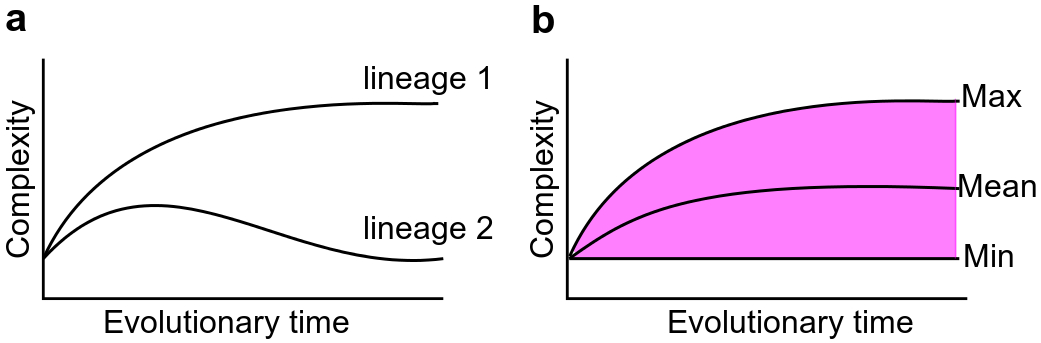
\includegraphics[width=12cm]{./Images/complexity_min.jpeg}
  \centering
  \caption{a) Two lineages with different complexity change through their evolutionary trajectories.
  b) Representation of the minimum, mean and maximum complexity of many lineages over evolutionary time in which the minimum stay constant while the mean and maximum increase.
Redrawn from \citep{Arthur2010}.
 }
  \label{fig:Complexity_min}
\end{figure}
%%%%%%%%%%%%%%%%%%%%%%%%%%%%%%%%%%%%%%%%%%%%%%%%%%%%%%%%%%%%%%%%%%%%%%%%%%%%%%%%%%%%%

\subsection{Complexity Increase in Development}

The increase in complexity in an organism during embryogenesis is probably one of the most intuitive processes of animal development.
It is commonly seen even as one of its defining characteristics.
Eric H. Davidson described the progressive increase in complexity as the "essence" of development \citep{Davidson2001}. Despite of the widely accepted view of complexity increase in development, there is no consensus of how to define it, much less on how to quantify it \citep{susan2000ontogeny}.

Using the number of cell types again as a proxy of morphological complexity, it can be said that during metazoan development, complexity increases as the zygote divides and differentiates into an adult with multiple cell types. 
This simple definition of complexity has its complications, as there is no clear criteria of how to define a cell type or how to determine when a new cell type has formed during development. 
For example, it could be that at the morphological level a cell seems to be undifferentiated, but when isolating it from its neighbour cells, it differentiates in an autonomous way into a specific cell type, suggesting that the cell fate was already determined without the necessity of further interactions with other cells.

\textbf{Talk about differentiation and determination?}

 
In addition, this definition does not take into account that embryos do not only get more cell types, but these cell types become organized in specific patterns in space and time in the embryo, which also could be considered as an increase in complexity over developmental time.

%%%%%%%%%%%%%%%%%%%%%%%%%%%%%%%%%%%%%%%%%%%%%%%%%%%%%%%%%%%%%%%%%%%%%%%%%%%%%%%%%%%%%%
%%\clearpage
%\begin{mdframed}[style=boxstyle,frametitle={Box1. On the similarity of complexity patterns between Evolution and Development}]\label{Box1:Haeckel&vonBaer}
%
%The connection between the increase in complexity during development and evolutionary time it has been largely discussed.
%Haeckel was one of the first who made explicit hypothesis about the connection between the development and evolutionary patterns.
%In what is known as Haeckel's "Biogenetic Law", he described development (or ontogeny), as a brief summary of the slow and long phylogeny \citep{haeckel1874menschen}.
%In his hypothesis, a "higher" organism would pass through a series of conserved developmental stages that represent ancestral forms. This view is also known as the "recapitulation theory".
%
%Karl Ernst von Baer, an Estonian naturalist, also formulated his own hypotheses, known as von Baer's laws \citep{vonBaer1828uber}. He stated that general characteristics develop before special characteristics (first law) and, opposed to Haeckel, that the embryo of a "higher" animal never resembles the adult of another animal form, but only his embryo (fourth law). 
%
%Apart from the differences in the "recapitulation" view, Haeckel and von Baer \citep{Richardson2002} they disagreed in the acceptance of evolution. 
%Haeckel's view was an evolutionary one, while von Baer's was not. Curiously, von Baer's arguments were used by Darwin in its "Origin" \citep{darwin1859origin} to support common ancestry and therefore, evolution.
%
%Now is evident that any of these hypotheses can be considered "laws", as they are not universal. They only apply to some characters, stages and levels of phylogenetic inclusiveness \citep{Richardson2002}. Nevertheless, both Haeckel and von Baer work represented the foundations of the comparative embryology field, which is in turn the basis of the modern evolutionary developmental biology (evo-devo).
%	\nomenclature{Evo-devo}{Evolutionary Developmental Biology}
%\end{mdframed}
%%%%%%%%%%%%%%%%%%%%%%%%%%%%%%%%%%%%%%%%%%%%%%%%%%%%%%%%%%%%%%%%%%%%%%%%%%%%%%%%%%%%%%

Defining a pattern as a specific distribution of cell types in a specific temporal window of embryonic development \citep{Salazar-Ciudad2004}, development can be conceptualized as the continuous transformation of one pattern into another.
The earliest pattern transformations usually establish the main axis or "compartments" of the embryo. For example, the anterior/posterior and dorsal/ventral axes in the fruit fly.
	\nomenclature{A/P}{anterior/posterior}
	\nomenclature{D/V}{dorsal/ventral}
Later pattern transformations define smaller compartments of the embryo, e.g, limbs, fingers  or internal organs.
As development proceeds, spatial compartments are progressively specified at an increasing finer resolution \citep{Davidson2001}.
Thus, a great part of pattern transformation is the partition of specific embryo compartments into smaller sub-compartments.

The compartmentalization of the embryo can be considered then an intrinsic property of development, and, as it is going to be mention in later sections, can be used as a proxy of complexity.

\subsection{Complexity at the molecular level}

At the molecular level, the increasing compartmentalization of the embryo during development can be seen as the progressive spatial restriction of gene expression to subsequently smaller regions in the embryo.
Sean Carroll conceptualizes this process\citep{Carroll2001} as:
%%%%%%%%%%%%%%%%%%%%%%%%%%%%%%%%%%%%%%%%%%%%%%%%%%%%%%%%%%%%%%%%%%%%%%%%%%%%%%%%%%%%
\begin{enumerate}
\item In early development, genes have a broad expression in the embryo and define the main axes of the body.
\item Later, genes define smaller compartments like organs and appendages (field-specific selector genes).
\item Finally, genes become expressed in specific cell types like muscle and neural cells (cell-type specific selector genes). 
\end{enumerate}
%%%%%%%%%%%%%%%%%%%%%%%%%%%%%%%%%%%%%%%%%%%%%%%%%%%%%%%%%%%%%%%%%%%%%%%%%%%%%%%%%%%%
%This would imply that in general, the area of expression of a gene in the embryo (relative to the area of the whole embryo)

If we consider again the number of cells as the complexity measure, we would expect that the increase in complexity over developmental time (as the number of cell types augments), should be associated with an underlying increase in complexity at the molecular level \citep{Arthur2010}, following the reasoning that:

%%%%%%%%%%%%%%%%%%%%%%%%%%%%%%%%%%%%%%%%%%%%%%%%%%%%%%%%%%%%%%%%%%%%%%%%%%%%%%%%%%%%
\begin{enumerate}
\item In development, the morphological complexity increases with time, as new cell types form.
\item Different cell-types are characterized by the differential expression of genes.
\item Therefore, the more cell-types an organism is formed of, more different combinations of expressed genes has to have (with the gene regulatory complexity this must entail).
\end{enumerate}
%%%%%%%%%%%%%%%%%%%%%%%%%%%%%%%%%%%%%%%%%%%%%%%%%%%%%%%%%%%%%%%%%%%%%%%%%%%%%%%%%%%%

The above reasoning has lead to some researchers to propose that the complexity of an organism resides in the regulatory machinery that ends into the differentiation of the diverse cell types \citep{Davidson2001}. 

For some, the combinatorial approach could also be seen as a solution for the "G-value paradox", as what really matters to be complex would not be how many genes an organism has, but how would these genes are differentially combined to produce more cell types in it. Another proposed solution is "gene co-option" in which a gene, usually after a duplication, evolves a new "function" different from its original one (REF Carrol 2003).

The differential gene expression in the various number of cell types are determined in great manner by the interplay of genes and their \textit{cis}-regulatory regions (DNA regions usually close to a gene which contains specific sequence motifs where proteins bind and affect its expression). The interaction between genes and their \textit{cis}-regulatory regions is sometimes referred as gene regulatory networks (GRNs) or "regulatory architecture" of the genome \citep{Davidson2001}.
	\nomenclature{GRN}{Gene Regulatory Network}
This approach to complexity relates to the "interaction among parts" definition of complexity mentioned at the beginning of this section.

In addition to the interaction between \textit{cis}-regulatory regions and genes, there are other gene expression regulatory mechanisms that have been proposed to be crucial in the origin of complex organisms.
This is the case of the microRNAs (miRNAs),
	\nomenclature{miRNAs}{microRNAs}
non-coding RNA molecules that negatively regulate gene expression.
After the observation that miRNAs are found only in protostomes and deuterostomes and not in sponges or cnidarians, and that they are specifically expressed in certain cell-types, tissues or organs, it was proposed that regulation of gene expression by miRNAs could have played a significant role in the origins of complex organs and "body plans" \citep{Sempere2006}.

\textbf{Other} authors highlight the importance of modules in facilitating the evolution of complex forms \citep{Carroll2001a}.


\subsubsection{Different types of developmental genes}

After acknowledging the importance of the spatio-temporal regulation of gene expression in development, it is useful to distinguish the type of genes that are directly involved in it.
More than fifty years ago, Jacques Monod and Fran\c cois Jacob \citep{Jacob1961} published in a seminal work a model of the genetic regulatory mechanism in bacteria.
The most important conclusion of this paper was the existence of "regulator" genes that control the production rate of proteins from "structural" genes, and that mutations in "regulator" genes affect the regulatory mechanism but not the structure of the regulated protein. In the same paper they suggested that these regulator genes may affect the synthesis of several different proteins \citep{Jacob1961}.

Nowadays the process of gene activation is known in great detail. The so-called "regulator genes" are now known as transcription factors, proteins that bind to DNA to promote or repress the transcription of a gene. 
%The discovery that 

The information for the spatio-temporal regulation of gene expression during cell differentiation requires however more than transcription factors, as the differentiation of a cell depends in a great manner of extracellular signals from its neighbouring context \citep{Gilbert2014}.
The molecule network involved in cell-cell communication, from the reception of a extracellular signal to the ultimate transcription of genes (usually going through many intermediate signal "transducers"), is known as a signalling pathway (see Figure \ref{fig:Signalling}).
Due to the importance of both transcription factors as signalling pathway genes in cell differentiation, a brief description of each follows.

%%%%%%%%%%%%%%%%%%%%%%%%%%%%%%%%%%%%%%%%%%%%%%%%%%%%%%%%%%%%%%%%%%%%%%%%%%%%%%%%%%%%%
\begin{figure}[h]
  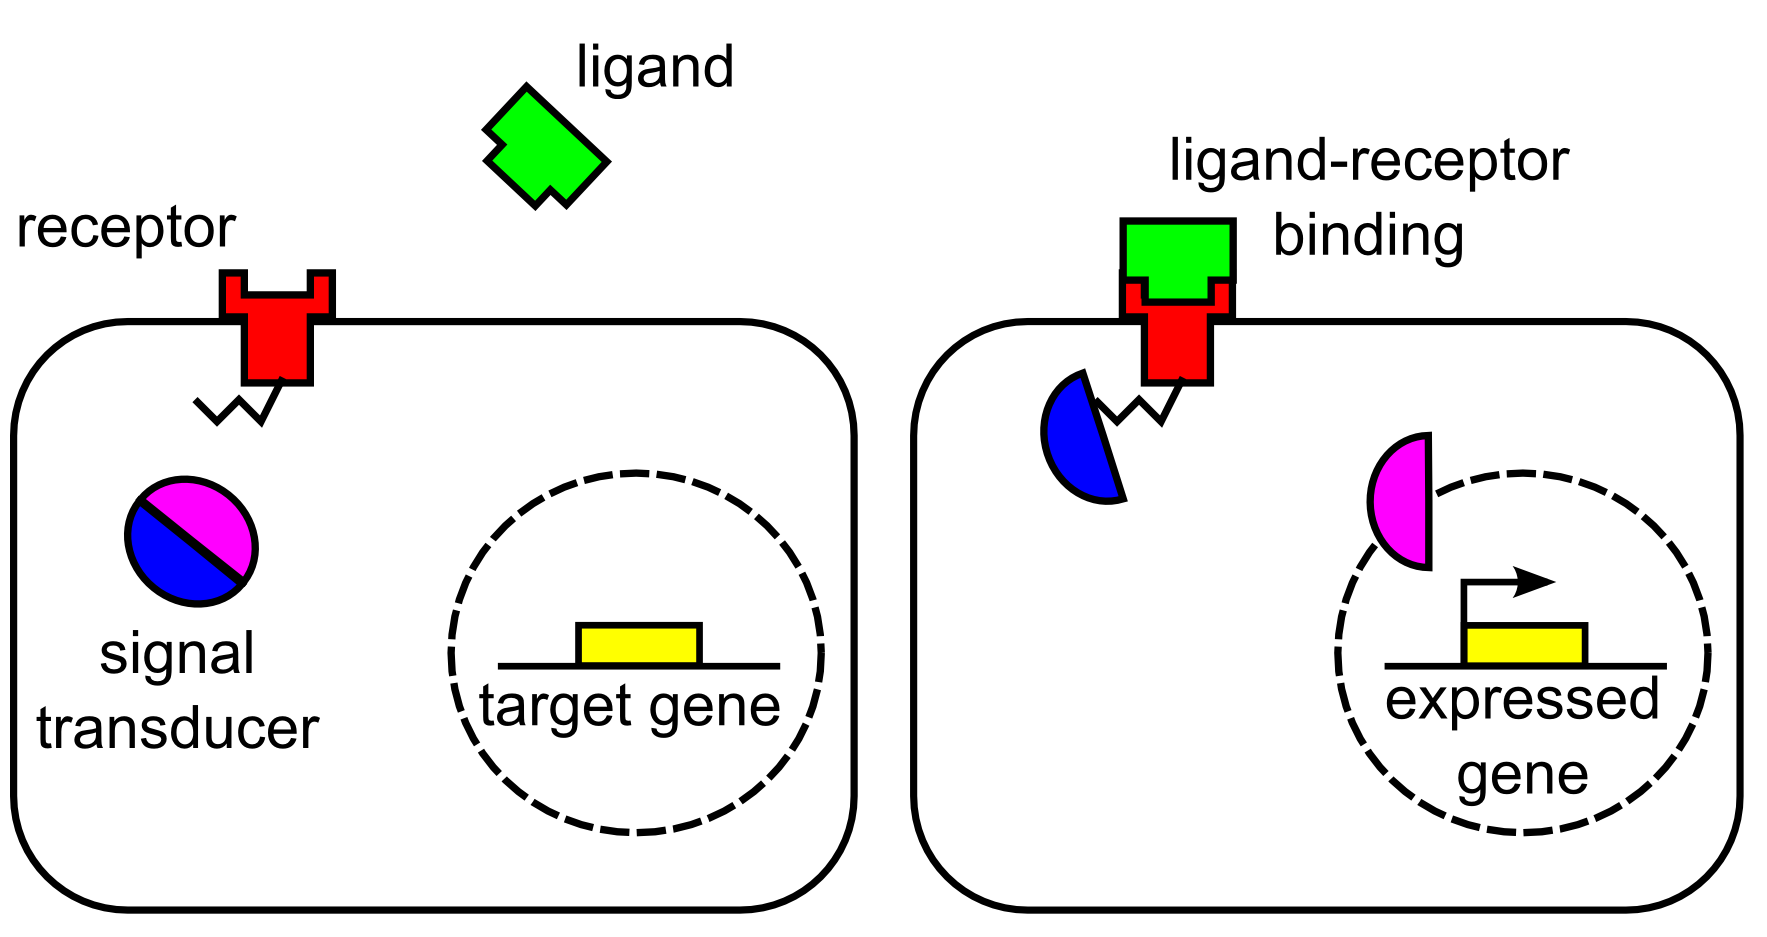
\includegraphics[width=10cm]{./Images/signalling.png}
  \centering
  \caption{
  Scheme of an hypothetical signalling pathway. Left: The extracellular ligand (green) is not bound to the membrane receptor (red) so the signal transducer protein (blue/magenta) is inactivated. In the nucleus (dashed circle) the target gene (yellow box) is inactive. Right: As the ligand binds to the receptor, the cytoplasmic domain (depicted as a zigzag tail) of the receptor change to an active conformation, cleaving the signal transducer. Part of the signal transducer acts as a transcription factor, going into the nucleus where activates the transcription of the target gene after binding to its regulatory region.
 }
  \label{fig:Signalling}
\end{figure}
%%%%%%%%%%%%%%%%%%%%%%%%%%%%%%%%%%%%%%%%%%%%%%%%%%%%%%%%%%%%%%%%%%%%%%%%%%%%%%%%%%%%%

\paragraph{Transcription factors} The transcription factors (TFs) are proteins that bind to specific regulatory regions, to induce or repress the expression of a gene.
Based on the secondary structure of the protein binding domain, TFs can b e classified in four main families: helix-turn-helix, helix-loop-helix, zinc finger and leucine zipper (\citep{Carroll2001}.
	\nomenclature{TF}{Transcription Factor}
	
The members of each family has been recognised in playing different roles in development. For example, it has been observed that in diverse metazoan species C2H2 zinc-figers TFs are over-represented in early development, as opposite to Homeobox TFs which are under-represented in the same period \citep{Schep2013}.
Hox genes (a subset of the Homeobox TF family) are involved in the A/P patterning of many metazoan groups. Intriguingly, these genes were found to have spatial collinearity in mice and flies (REF). That means that the A/P expression of the Hox genes reflects their physical order along the chromosome.
At the time of its discovery, collinearity of Hox genes were considered as a master plan for A/P patterning in animals (REF).
However, after Hox genes were investigated in more species it became clear that in some species with Hox genes collinearity is not always present, and some species do not have Hox genes at all (REF).

\paragraph{Signalling pathway genes} Signalling pathways are usually a complex network of molecules including extracellular diffusible signals, membrane receptors, intermediate signal transducer molecules and transcription factors.
Signalling pathways usually begin with a extracellular signal that causes a conformational change in its cell membrane receptor after binding to it.
The new conformation results in enzymatic activity in the cytoplasmic domains of the receptor protein, that phosphorylate other cytoplasmic proteins.
Finally, one or more activated transcription factors induce or repress specific gene activity \citep{Gilbert2014}.

Signalling pathways recurrently used during animal development are the Wnt, FGF and Shh pathways (for a detailed description of each signalling pathway, see \citep{Gilbert2014}.
For example, the Shh pathway plays a fundamental role in the fruit fly segment polarization(REF) and wing development (REF), and in vertebrate limb (REF) and tooth development \citep{Jernvall2000b}.

\subsection{Complexity in informational terms}

\cite{Davidson2001} used the GRN concept in addition to others to explain development (and evolution) on informational terms. He said that development (which is the outcome of spatial and temporal series of differential gene expression) is controlled by a hardwired regulatory program built into the DNA and the metric of complexity is the diversity of the programs of gene expression that are "installed and executed" as the embryo develops. As Davidson, other authors have used informational/computational analogies to define development \citep{Apter1965,monod2012cytodifferentiation,mayr1997evolution} 

To illustrate how the complexity of a regulatory network or "program" can increase in evolution (but a similar case could be said for development), Davidson describes an imaginary example:
an early evolutionary state consists of a small gene battery (set of functionally linked genes expressed in concert) encoding proteins used for some differentiated cell type, which is activated by a small number of genes encoding transcription factors. The network activating the gene battery is itself controlled by a single upstream gene.
In subsequent evolutionary states, the whole structure is said to become more complex as: the battery of genes is now used in some pattern formation system, new batteries of genes appear, new regulatory genes and new \textit{cis}-regulatory regions are introduced  \citep{Davidson2001}.

Even when in this kind of examples would seem easy to discern a simple GRN from a complex one just from its topology, the high intricacy of real biological systems make this an extremely difficult if not impossible task. 

%%%%%%%%%%%%%%%%%%%%%%%%%%%%%%%%%%%%%%%%%%%%%%%%%%%%%%%%%%%%%%%%%%%%%%%%%%%%%%%%%%%%%
\begin{figure}[h]
  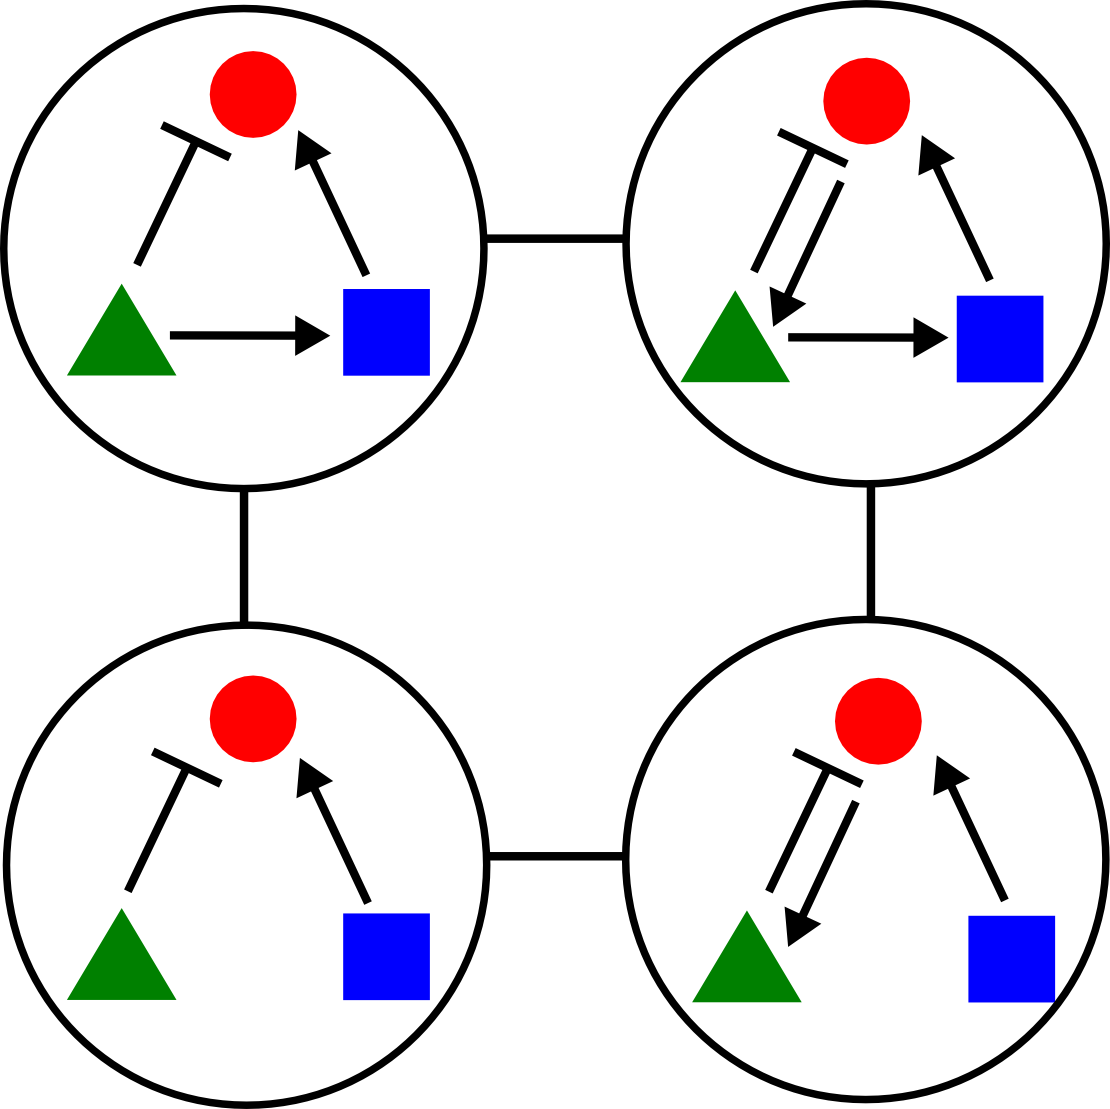
\includegraphics[width=5cm]{./Images/GRNs.png}
  \centering
  \caption{
  Some GRNs . Cotterel and Harpe calculated... \citep{Cotterell2010}
 }
  \label{fig:GRNs}
\end{figure}
%%%%%%%%%%%%%%%%%%%%%%%%%%%%%%%%%%%%%%%%%%%%%%%%%%%%%%%%%%%%%%%%%%%%%%%%%%%%%%%%%%%%%

There are also important critiques of this informational approach. First, using an informational analogy to describe development implies the distinction between a "hardware" and a "software".
The "hardware" would consist of the genome structure, regulatory components, cells, organs, etc., and the "software" would be the GRNs or the set of instructions that directs the performance of specific operations.
For biological systems, this distinction is misleading, as there are recurrent feedback between its "hardware" and "software", so that the structure of development processes change through development \citep{susan2000ontogeny,Salazar-Ciudad2009,Jaeger2014devmech}.


\subsection{Complexity in terms of dynamical systems theory}

Estimating the combinatorial possibilities of a small set of regulatory genes, considering that each gene can regulate (whether positively or negatively) more than one gene's expression in addition to its own, could result in an astronomic number of possible gene topologies (see Figure \ref{fig:GRNs}).
Also feedback effects and non-linear regulation of gene expression make the prediction of changes in regulatory states hard or even impossible to predict \citep{Jaeger2014devmech}.

To overcome this limitations, some authors have propose to use dynamical systems theory, which deals with a complex system with many interacting components (a dynamical system), by representing its state as a point in a multidimensional space \citep{Alberch1991,ForgacsandStuartA.Newman.2005,Jaeger2014devmech}. 
To illustrate this we could think of a specific cell type, with \textit{n} number of genes, which its cell state depends on the expression of each of the genes.
The simpler case we could imagine would be a cell with only two genes. In this case, the cell would be in a two-dimensional "state space" (also called "phase space").

Importantly, the dynamical system is governed by the relations between its components \citep{ForgacsandStuartA.Newman.2005}. In our example the relations would be represented by the interaction between genes, namely the gene regulatory network (GRN). 
If in our example the expression level of one gene is affected by the expression level of the other gene, the system will not stay in any particular state, but it will change until it reaches a "stable steady state", in which the level of both genes are at equilibrium. 
Given a specific GRN, the number of stable states would represent the possible differentiation states a cell can achieve (REF Slack book)

Many modifications of the GRN would not have consequences in the ultimate differentiation state, as it will converge to the same "attractor" point.
However, some modifications (or mutations) could produce a change in the "state space" leading to the formation of a new stable state (i.e., a new cell type).
So within the framework of the dynamical systems theory, and keeping the number of cell types as our measure of complexity, there would be an increase in complexity when a mutation would change the gene regulatory machinery so that a new stable steady state is formed.


\textbf{Make a figure?}
%-nothing about spatial or statistical approach like our disparity measure
%- explain something about non-genetic components? (Newman, Gabor and Forgacs, Alberch, Isaac)

%\clearpage
%	\clearpage 
\section{Adaptation}
	
%In many texts however, adaptation is not clearly defined (leading to ambiguity) or is often used in biological irrelevant contexts \citep{Dobzhansky1968}.  
%Even in Darwin's \textit{Origin}, where it is a central concept, adaptation is not explicitly defined throughout the text \citep{darwin1859origin}.
In this section, I will start with the definition of the concepts of adaptation (although there are more than one definition of adaptation; \citealp{endler1986natural}), and natural selection. Then I will introduce some of the methods that are used to estimate adaptation, with a focus on molecular methods.

\subsubsection{On the concept of adaptation}
%Measuring adaptation is a central theme in evolutionary biology.
Usually adaptation refer to two different things, to an adaptive trait or to the process to become adapted \citep{endler1986natural}.
George Gaylord \citet{Simpson1953} defined adaptation in the following way: 

"\textit{an} adaptation is a characteristic of an organism advantageous to it or to the conspecific group in which it lives, while adaptation or the process of adaptation is the acquisition within a population of such individual adaptation" (italics by the author)

An adaptation (i.e., an adaptive trait) is usually related to a specific function of the organism. For example, the beak variations (in size, width and depth) in the Darwin's Galapagos finches, a classic example of adaptive traits, are related to the alimentary function of the finches, so that each species is specialized in a specific diet.
The notion of adaptation existed before Darwin, but since Darwin it is closely related to the concept of natural selection. Under the current evolutionary framework, an adaptation, arising due to intrinsic natural variation, will be fixed in a population by natural selection due to the advantage it confers to their bearer organisms.

%We say an organism is adapted to an environment when it is able to live and reproduce in it. A related concept is adaptedness, or "the degree to which an organism is adapted to an environment" \citep{Dobzhansky1968}.
%
%In here, I refer to adaptation as a phenotypic character (or modification in a phenotypic character) that arise by natural selection in response to the environment, or other external factor.
%
%Since Darwin, the concepts of adaptation and natural selection usually come together. There has been a long standing controversy on the relationship between natural selection and adaptation.
%For some authors like Barton et al., adaptation is "a trait that functions to increase fitness and that evolved for that function" and that can be only caused by natural selection (REF Barton).
%Other authors however, consider that an adaptation might originate only by chance and natural selection only addresses the spread of adaptive variants (Williams, Gould and Vrba, Alberch).


\subsubsection{Natural selection}

Charles Darwin, in its 1859's \textit{Origin}, defined Natural selection as follows:
%%%%%%%%%%%%%%%%%%%%%%%%%%%%%%%%%%%%%%%%%%%%%%%%%%%%%%%%%%%%%%%%%%%%%%%%%%%%%%%%%%%
\begin{flushleft}
\leftskip3em
\rightskip\leftskip
\footnotesize{
\textit{
" Owing to this struggle (for life), variations, however slight and from whatever cause proceeding, if they be in any degree profitable to the individuals of a species (...) will tend to the preservation of such individuals, and will generally be inherited by the offspring. The offspring, also, will thus have a better chance of surviving, for, of the many individuals of any species which are periodically born, but a small number can survive. I have called this principle,
by which each slight variation, if useful, is preserved, by the term Natural Selection"} \citep{darwin1859origin}.
}
\end{flushleft}
%%%%%%%%%%%%%%%%%%%%%%%%%%%%%%%%%%%%%%%%%%%%%%%%%%%%%%%%%%%%%%%%%%%%%%%%%%%%%%%%%%%

More recently, and following the Darwininan concept of natural selection, Jhon A. \citet{endler1986natural}, defined it as a process in which, given that a population has:

\vspace{3mm}
%%%%%%%%%%%%%%%%%%%%%%%%%%%%%%%%%%%%%%%%%%%%%%%%%%%%%%%%%%%%%%%%%%%%%%%%%%%%%%%%%%%%%%%
\begin{enumerate}[label=\textit{\alph*.}]
\item \textbf{variation} among individuals in some attribute or trait;
\item \textbf{fitness differences} (consistent relationship between that trait and mating ability, fertilizing ability, fertility, fecundity, and, or, survivorship);
\item  \textbf{inheritance} (consistent relationship, for that trait, between parents and their offspring, which is at least partially independent of common environmental effects).
\end{enumerate}
%%%%%%%%%%%%%%%%%%%%%%%%%%%%%%%%%%%%%%%%%%%%%%%%%%%%%%%%%%%%%%%%%%%%%%%%%%%%%%%%%%%%%%%
\vspace{3mm}
Then:
\vspace{3mm}
%%%%%%%%%%%%%%%%%%%%%%%%%%%%%%%%%%%%%%%%%%%%%%%%%%%%%%%%%%%%%%%%%%%%%%%%%%%%%%%%%%%%%%%
\begin{enumerate}
\item the trait frequency distribution will differ among age classes or life-history stages, beyond that expected from ontogeny;
\item\ if the population is not at equilibrium, then the trait distribution of all offspring in the population will be predictably different from that of all parents, beyond that expected
from conditions a and c alone.
\end{enumerate}
%%%%%%%%%%%%%%%%%%%%%%%%%%%%%%%%%%%%%%%%%%%%%%%%%%%%%%%%%%%%%%%%%%%%%%%%%%%%%%%%%%%%%%%
\vspace{3mm}

Conditions a, b, and c are necessary and sufficient for the process of natural selection to occur, and these lead to deductions i and ii \citep{endler1986natural}.

Condition a relates to phenotypic changes across generations. Importantly, phenotypic changes, whether new characters or modifications of existing characters in the adult/larva, are produced from changes in development.
For example, the difference in the beak size and shape between Galapagos Darwin's finches has been shown to be regulated by the differential expression of the genes CaM and BMP4 during development \citep{Abzhanov2006}.

Therefore, even when natural selection acts in the adult/larva phenotype, the changes that lead to an adaptation should be traceable during the development of such trait.

\subsubsection{Methods to detect natural selection}

There are many different methods designed to detect natural selection in natural populations. Jhon A. Endler classified ten different methods with diverse ability to detect natural selection \citep{endler1986natural}. Some of these methods test directly the conditions (b and c) required by natural selection, while others test the predicted outcome of natural selection in a population.

There are many studies that have aimed to detect natural selection directly in the phenotype. Usually, these studies are based on the estimation of selection gradients of a quantitative trait (a measurable phenotype that usually depends on the cumulative actions of many genes and the environment). A selection gradient of a trait refers to the relation of the trait values and fitness. Is calculated as the slope of a linear regression of fitness on the trait value \citep{barton2007evolution}.
Most of these studies are based on the analysis a single trait or a small number of traits of an organism \citep{Hoekstra2001,Hereford2004} which are usually selected already under the suspicion to be adaptive. However, there is practically no study that has attempted to estimate natural selection over the entire organism.

Among the methods that test the predicted outcome of natural selection we find the molecular methods. The molecular methods are based on the assumption that changes leading to an adaptation are (at least partially) caused by DNA mutations and that the effects of natural selection could be traceable looking at the DNA sequence.
There is an entire field within evolutionary biology, namely molecular evolution, dedicated to explain the evolutionary sequence changes in molecules as DNA, RNA and proteins.
	\nomenclature{DNA}{Deoxyribonucleic acid}
	\nomenclature{RNA}{Ribonucleic acid}

In the next sections, due to its relevance in this work I will only focus on the molecular methods to detect natural selection.

\subsection{Molecular evolution}

The theoretical basis of the molecular evolution field includes concepts from evolutionary biology and population genetics. At the DNA level, any transmissible change in the sequence is considered a mutation. 
The most simple change is a point mutation, also called single nucleotide polymorphism (SNP),
	\nomenclature{SNP}{Single nucleotide polymorphism} 
which is a change in a single nucleotide in the DNA sequence of a locus in an individual.

Variation at a particular DNA site within the individuals of a species or population is referred as polymorphism, while divergence refers to variation at a specific DNA site in individuals from different species.
%
SNPs occur in non-coding and coding DNA sequences. A SNP that occurs in a coding sequence is classified in two categories, depending on its effect on the protein sequence: i) synonymous mutation and ii) non-synonymous mutation.
A synonymous mutation does not affect the amino-acid sequence of the protein (although it can affect its function 
	\citep{Kimchi-Sarfaty2007} or the gene transcriptional efficiency \citep{Xia1996}.
A non-synonymous mutation affects the amino-acid sequence of the protein whether by changing a single amino-acid (missense mutation) or by producing a stop codon (non-sense mutation) which results in a truncated version of the protein.
%
As the non-synonymous mutations can affect dramatically the structure and function of the protein, it is expected that most non-synonymous mutations have a negative fitness effect.
However, it is also expected that a fraction of non-synonymous mutations would have a positive fitness effect that, depending on the strength of the fitness effect and several population genetics parameters, could lead to the fixation of that mutation in the population (i.e., adaptive substitutions).

An important branch of the molecular evolution field is dedicated to the identification of adaptive substitutions in a species, which has lead to the development of many statistical tests, which are based on the neutral theory of evolution, proposed by Kimura
	\citep{Kimura1968}.

\subsubsection{Neutral theory of evolution}
In 1968, Mooto Kimura calculated the average rate of nucleotide substitutions in the evolutionary history of mammals.
The result of his calculations was that, on average, one nucleotide has been substituted every 2 years.
For him, this very high rate of substitution was only explainable if most mutations were almost neutral in natural selection 
	\citep{Kimura1968}.
which was in contradiction with the prevailing view at the time that practically no mutations were neutral.

In 1969, Kimura proposed that the majority of amino acid substitutions that occurred in proteins are the result of random fixation of selectively neutral or nearly neutral mutations  \citep{Kimura1969}. In the same year, King and Jukes \citep{King1969} independently proposed practically the same hypothesis.
%
Two important assumptions of the neutral theory of molecular evolution were:

%%%%%%%%%%%%%%%%%%%%%%%%%%%%%%%%%%%%%%%%%%%%%%%%%%%%%%%%%%%%%%%%%%%%%%%%%%%%%%%%%%%%%%%
\begin{enumerate}
\item Deleterious and adaptive mutations are rapidly purged and fixed in a population respectively.
\item Polymorphism is a transitory phase between random fixation or extinction due to genetic drift.
\end{enumerate}
%%%%%%%%%%%%%%%%%%%%%%%%%%%%%%%%%%%%%%%%%%%%%%%%%%%%%%%%%%%%%%%%%%%%%%%%%%%%%%%%%%%%%%%

Importantly, the neutral theory provided a set of testable predictions, providing a null-hypothesis for adaptive molecular evolution.
%This allowed the development of statistical methods to detect adaptive changes.
%i.e., we can say that a sequence has been under positive selection if the amount of changes exceeds the number of changes expected only by neutral evolution.
%Since the 1990's one of the most popular tests has been the McDonald-Kreitman test (MKT), which estimates the proportion of the adaptive substitution resulted from natural selection.

\subsubsection{From neutral to nearly neutral theories}

In the subsequent decades after the proposal of the neutral theory of molecular evolution, much more protein sequence data became available, which made evident the great variation in the evolution rate of proteins.
To account for this, Kimura and Ohta stated that "functionally less important molecules or parts of a molecule evolve faster than more important ones" \citep{Kimura1974}.
Then, Ohta propose that slightly deleterious mutations might be common in amino acid substitutions \citep{Ohta1973}. Later, it was proposed that half of the protein substitutions would be advantageous and the other half deleterious \citep{gillespie1994causes}.
Therefore, the neutral model was replaced by a nearly neutral model with only deleterious substitutions, which in turn was replaced by one with a mixture of positive and negative effects \citep{Ohta1996}.

At the end of the 1970's comparative analyses of protein sequence data began to be replaced for analyses on DNA sequence data, which revealed that synonymous substitutions within coding regions are more frequent than non synonymous (those that change an amino acid) substitutions.
%
From the early 1990s, the expectations of the nearly neutral theory at the DNA sequence level are that substitutions in non coding DNA and synonymous substitutions in coding regions are neutral and amino acid substitutions can be deleterious, neutral or advantageous \citep{Ohta1996}. Statistical methods were then devised to test such expectations.

\subsection{Estimating adaptation at the molecular level}
One of the most popular tests to estimate adaptation at the molecular level has been the McDonald-Kreitman test (MKT), which is used to detect adaptive substitutions comparing the relative numbers of synonymous and non-synonymous differences within a species with those numbers between closely related species.

\subsubsection{McDonald-Kreitman test}

\nomenclature{MKT}{MacDonald-Kreitman test}

John H. McDonald and Martin Kreitman developed this test in 1991 when analysing the divergence in the Alcohol dehydrogenase (Adh) locus in three \textit{Drosophila} species	\citep{McDonald1991}. 
%
The main assumption of the MKT is that the substitutions in a protein are neutral if the inter-specific ratio of non-synonymous ($Dn$) to synonymous ($Ds$) changes is equal to the intra-specific ratio of non-synonymous ($Pn$) to synonymous ($Ps$) changes (i.e. $Dn/Ds = Pn/Ps$).
Any departure from this equality would imply the action of positive or negative selection.
%
Importantly, MKT assumes for simplicity that non-synonymous mutations are either strongly deleterious, neutral or strongly advantageous \citep{McDonald1991}.
%
%Mutations under positive selection therefore would be expected to spread through a population rapidly so they would not contribute to polymorphism but only to divergence substitutions.

In other words, this method assumes that a protein in a given phylogeny has a specific substitution rate for synonymous and another for non-synonymous substitutions. Therefore, when comparing two proteins from two different species that have evolved under neutral conditions, the \textit{total} number of each type of substitutions would depend on the time since the separation between species. If the proteins are from individuals from the same species, it would depend on the time elapsed since the separation of the within-species branches of the phylogeny.
However, the ratio of non-synonymous to synonymous substitutions is expected to be the same in both inter-specific and intra-specific cases. 
In the case of non-synonymous mutations under positive selection (synonymous mutations are expected to be always neutral), the equality of these ratios would disappear. As mutations under positive selection are expected to spread through a population rapidly (and are not expected to very common) they are not expected to be present as polymorphic (i.e., intra-specific) variation, but only as divergent (i.e., inter-specific) one.

Therefore, in the presence of mutations under positive selection, the ratio of non-synonymous to synonymous variation within species should be lower than the ratio of non-synonymous to synonymous variation between species (i.e. $Dn/Ds > Pn/Ps$; see Fig. \ref{fig:MKT}). 
On the contrary, if the observed ratio of non-synonymous to synonymous variation between species is lower than the ratio of non-synonymous to synonymous variation within species (i.e., $Dn/Ds < Pn/Ps$) then negative selection is at work.
	\nomenclature{$Dn$}{Non-synonymous (inter-specific) divergence per site}
	\nomenclature{$Ds$}{Synonymous (inter-specific) divergence per site}
	\nomenclature{$Pn$}{Synonymous (intra-specific) polymorphism per site}
	\nomenclature{$Ps$}{Synonymous (intra-specific) polymorphism per site}
%

%%%%%%%%%%%%%%%%%%%%%%%%%%%%%%%%%%%%%%%%%%%%%%%%%%%%%%%%%%%%%%%%%%%%%
\begin{figure}[h]
  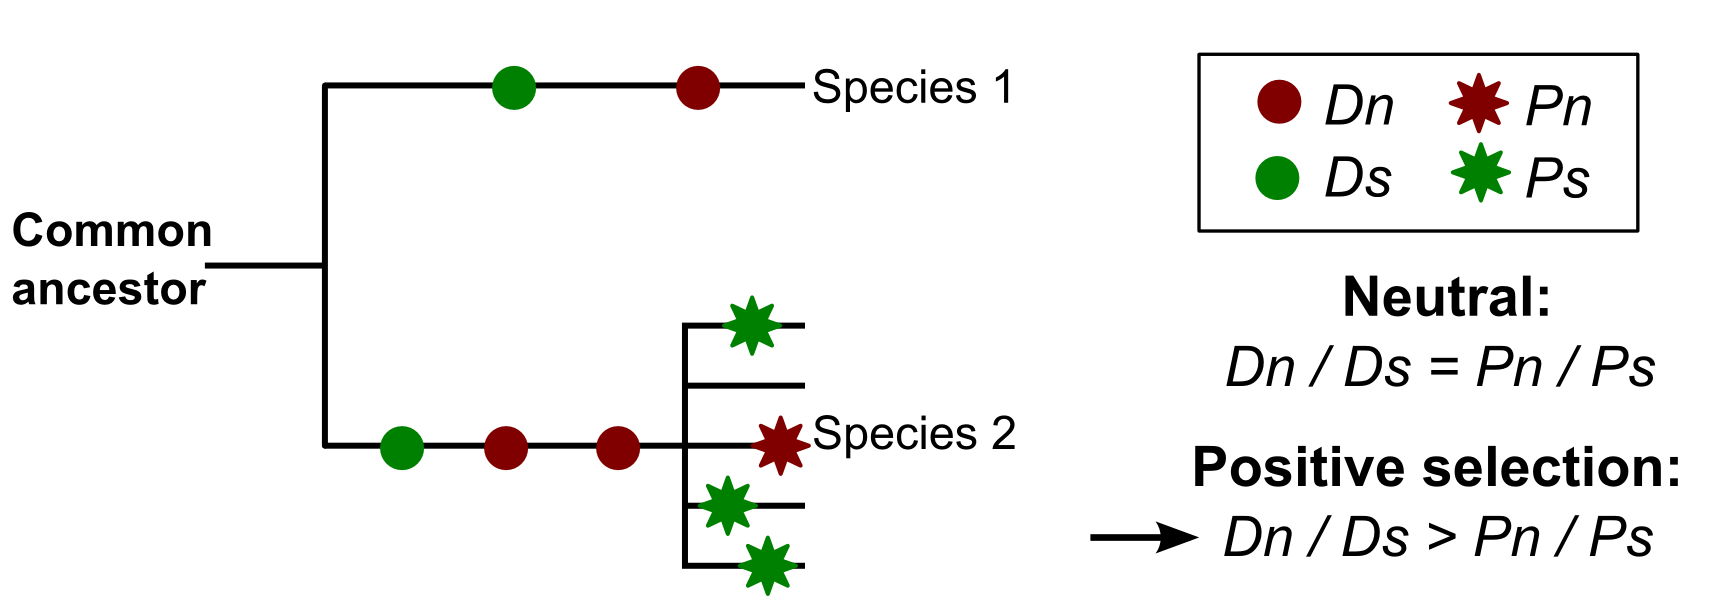
\includegraphics[width=10cm]{./Images/MKT.png}
  \centering
  \caption{\textbf{McDonald-Kreitman Test (MKT).} MKT compares the ratio of non-synonymous ($Dn$; red circle) to synonymous ($Ds$; green circle) divergence ($Dn/Ds$) to the ratio of non-synonymous ($Pn$; red star) to synonymous ($Ps$; green star) polymorphic changes ($Pn/Ps$). Positive selection is detected when $Dn/Ds > Pn/Ps$, as in the example shown in the left.
   }
  \label{fig:MKT}
\end{figure}
%%%%%%%%%%%%%%%%%%%%%%%%%%%%%%%%%%%%%%%%%%%%%%%%%%%%%%%%%%%%%%%%%%%%%

Although the MKT has been proved robust to many sources of error (e.g., variation to mutation rate across the genome), it can be affected by the presence of slightly deleterious mutations or demography \citep{Messer2013,Eyre-Walker2006a}. 
%
The effect of slightly deleterious mutations is related to the effective population size ($N_{e}$). In a population with a low $N_{e}$, slightly deleterious mutations would have more probabilities of fixation by random genetic drift contributing more to polymorphism than to divergence, underestimating the proportion of adaptive changes \citep{Messer2013}.

Recently, sophisticated methods based on the MKT have been developed to correct for underestimation of adaptive evolution in the presence of slightly deleterious mutations. 


\subsubsection{Distribution of Fitness Effects}

%To have a more precise estimate of the proportion of adaptive substitutions it is important to consider the relative contributions of the different types of mutations, based on their fitness effects.
Even when for simplicity the mutation effects are usually classified in strongly advantageous, neutral, and strongly deleterious, there is actually a continuum of selective effects, from strongly deleterious, 
to highly adaptive mutations, with weakly deleterious, neutral and slightly adaptive mutations in between \citep{Eyre-Walker2007}.

The relative frequencies of all these types of mutations is called the Distribution of Fitness Effects (DFE).
	\nomenclature{DFE}{Distribution of Fitness Effects}
In order to know the DFE, a few experimental approaches exist. The most direct method is whether to induce \citep{Sanjuan2004} or to collect \citep{MUKAI1964} spontaneous mutations and assay their effects (fitness) in the laboratory.
As it can be expected, these experiments require many generations to gather sufficient data, so these approaches have been used mainly in micro-organisms \citep{Eyre-Walker2007}.
A caveat of these experimental approaches is that, in order to identify the effect of a mutation, its effect has to be detectable in a fitness assay. In fitness assays however, only effects with relatively large effects are usually detected. Therefore, these methods give valuable information for mutations with relatively large effects.

An alternative approach is to infer the DFE by analysing patterns of DNA sequence differences at intra and inter-specific level (polymorphism and divergence respectively).
The methods using this approach rely mainly on two assumptions:
%%%%%%%%%%%%%%%%%%%%%%%%%%%%%%%%%%%%%%%%%%%%%%%%%%%%%%%%%%%%%%%%%%%%%%%%%%%%%%%%%%%%%%%
\begin{enumerate}
\item  the probability that a mutation spreads to a certain frequency in a population (or to fixation) depends on the strength of selection (positive or negative) acting on it.
Severely deleterious mutations have lower probability to reach a high frequency in a population.
\item\ the efficiency of selection depends on the effective population size. 
With a high effective population size, selection is more efficient and a smaller proportion of mutation will behave as effectively neutral.
\end{enumerate}
%%%%%%%%%%%%%%%%%%%%%%%%%%%%%%%%%%%%%%%%%%%%%%%%%%%%%%%%%%%%%%%%%%%%%%%%%%%%%%%%%%%%%%%
%i) the probability that a mutation spreads to a certain freq in a population (or to fixation) depends on the strength of selection (positive or negative) acting on it.
%Severely deleterious mutations have lower probability to reach a high frequency in a population.
%ii) the efficiency of selection depends on the effective population size. 
%With a high effective population size, selection is more efficient and a smaller proportion of mutation will behave as effectively neutral.
%
The "absolute strength" of selection on a mutation is then measured as $N_{e}s$, the product of the effective population size ($N_{e}$) by the selection coefficient ($s$) of the mutation. Mutations with $N_{e}s$ much less than 1 are effectively neutral, while $N_{e}s$ greater than 100 have no chance to appear as polymorphism \citep{Eyre-Walker2007}.
	\nomenclature{$N_{e}$}{Effective population size}
	\nomenclature{$s$}{Selection coefficient}

\subsubsection{DFE-alpha method} \label{alpha}

Eyre-Walker and collaborators proposed a method to estimate both the DFE and the proportion of adaptive nucleotide substitutions ($\alpha$) using polymorphism and divergence data \citep{Eyre-Walker2009}.
More specifically, they use the polymorphism site frequency spectrum (SFS) to estimate the DFE and then use this estimated DFE to estimate the proportion of substitutions under positive selection between species.
	\nomenclature{$\alpha$}{Proportion of adaptive nucleotide substitutions}
	\nomenclature{SFS}{Site Frequency Spectrum}
%
To estimate the DFE from the SFS, they developed a maximum likelihood method using the expected allele frequency distribution based on a variation of the Fisher-Wright transition matrix (for more details, see \citealp{Keightley2007,Eyre-Walker2009}).

This method, assumes that there are two types of nucleotide sites: 
i) sites at which all mutations are neutral and ii) sites at which some of the mutations are subject to selection (positive or negative).
Also it is assumed that any new adaptive mutation in a population would not be detected in the polymorphic phase but only in the divergent one (as the advantageous mutations would fix rapidly in a population), and that the DFE can be represented with a gamma distribution (Figure \ref{fig:Gamma}).

%%%%%%%%%%%%%%%%%%%%%%%%%%%%%%%%%%%%%%%%%%%%%%%%%%%%%%%%%%%%%%%%%%%%%
\begin{figure}[h]
  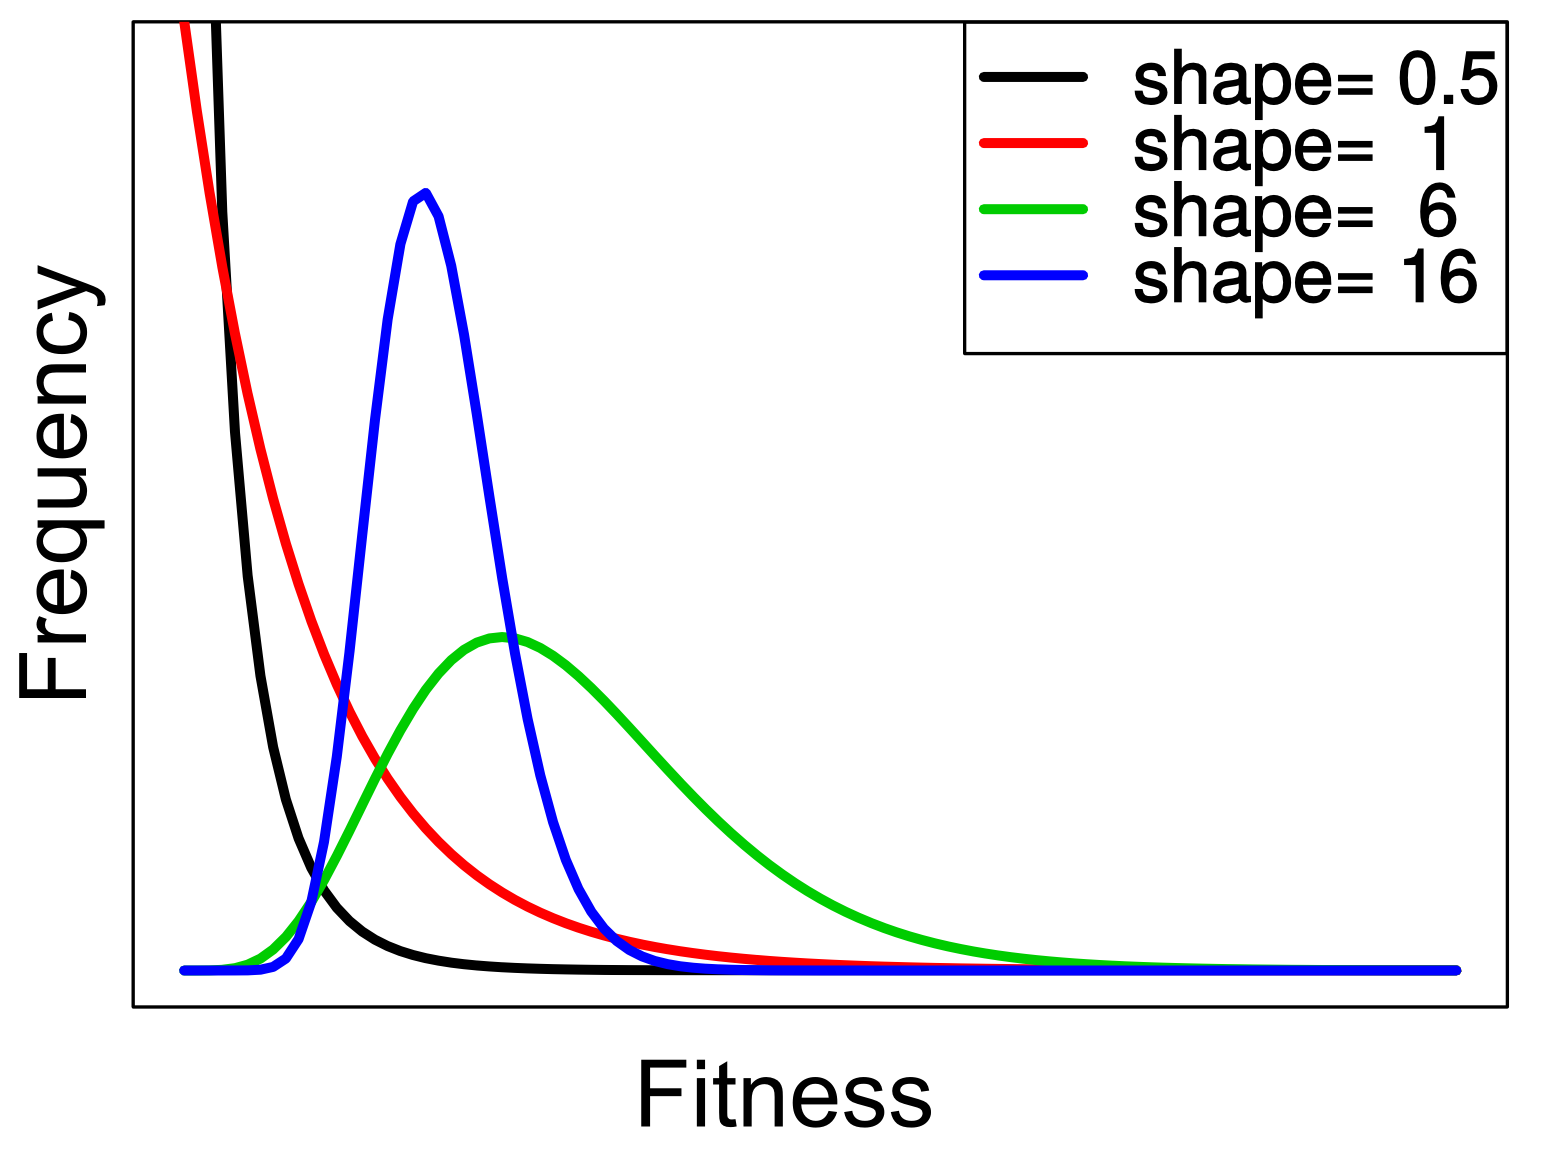
\includegraphics[width=6cm]{./Images/Gamma_dist_2.png}
  \centering
  \caption{Example of different Distribution of Fitness Effects (DFE) represented by a gamma distribution. Many distributions can be represented by modifying the shape parameter of a gamma distribution, from a leptokurtic (shape parameter less than 1) to an exponential (shape parameter equal to 1) or a skewed normal distribution (shape  greater than 1).
   }
  \label{fig:Gamma}
\end{figure}
%%%%%%%%%%%%%%%%%%%%%%%%%%%%%%%%%%%%%%%%%%%%%%%%%%%%%%%%%%%%%%%%%%%%%

The divergence at the neutral sites is then proportional to the mutation rate per site and the predicted divergence at the selected sites (in the absence of advantageous mutations) is proportional to the product of the mutation rate together with the average fixation probability of a selected mutation.
This probability of fixation is is inferred based on the DFE and other parameters estimated from the polymorphism data analysis \citep{Eyre-Walker2009}.
The difference between the observed and predicted divergence therefore estimates the divergence due to adaptive substitutions.
%
Using this method Eyre-Walker and collaborators estimated that in \textit{Drosophila} genes approximately 50\% of amino acid substitutions and approximately 20\% of substitutions in introns are adaptive \citep{Eyre-Walker2009}.

Messer and Petrov performed molecular evolution simulations to test if the estimates of different tests, like the MKT and the more sophisticated DFE-alpha, are accurate under different realistic gene-structure and selection scenarios \citep{Messer2013}, specially in the presence of genetic draft (stochastic effects generated by recurrent selective sweeps at closely linked sites)
and background selection (interference among linked sites by lightly deleterious polymorphisms).
%
They found that in the presence of slightly deleterious mutations, MKT estimates of $\alpha$ are severely underestimated and that DFE-alpha is very accurate to calculate $\alpha$ even in the presence of genetic draft, background selection or demography changes \citep{Messer2013}.
%

Methods lilke the DFE-alpha would be ideal to analyse intra-specific variation in a natural population at a genomic level. In the last years, different population-genomic projects have sequenced, in different species, the genome of many individuals of a population (or a set of populations) \citep{The1000GenomesProjectConsortium2010,Mackay2012,Pool2012,Wallberg2014}, providing a valuable resource of genomic polymorphism data at the population level.
One of these projects is the \textit{Drosophila melanogaster} Genetic Reference Panel (DGRP), a publicly available tool for molecular population genomic analyses, briefly described in the following subsection.
%This is because genetic draft leaves similar signatures to a recent population expansion, namely distortions of the SFS at synomymous sites, and the DFE-alpha interprets these SFS distortions as being a consequence of demography and attempts to correct for it.
%Importantly, this caveat in using the DFE-alpha is only relevant when demography changes wants to be estimated, but not when alpha is the parameter of interest, as in here.
%
%\subsubsection{Inferring natural selection using a population genomics approach}
%
%For taking advantage of these new methods that infer adaptation combining polymorphism and divergence data, a populations genomics approach is necessary. 
%In the last years, different projects have sequenced, in different species, the genome of many individuals of a population (or a set of populations) \citep{The1000GenomesProjectConsortium2010,Mackay2012,Pool2012,Wallberg2014}, providing a valuable resource of genomic polymorphism data at the population level.
%
%In this study, I used data from the \textit{Drosophila melanogaster} Genetic Reference Panel (DGRP) \citep{Mackay2012}, which consists of inbred \textit{D. melanogaster} lines.
%Importantly, the lines are derived from a single outbred population, so they capture natural variation (as genetic polymorphism) and are ideal to use with methods like the DFE-alpha. 
%
%	\nomenclature{DGRP}{The \textit{Drosophila melanogaster} Genetic Reference Panel}


\subsection{The \textit{Drosophila melanogaster} Genetic Reference Panel} 
\label{DGRP}
	\nomenclature{DGRP}{The \textit{Drosophila melanogaster} Genetic Reference Panel}

%
DGRP consists of 192 inbred strains derived from a single outbred \textit{Drosophila melanogaster} population.
The inbred lines were constructed from collected mated females from a Raleigh (North Carolina, USA) population, followed by 20 generations of full-sibling inbreeding of their progeny \citep{Mackay2012}.
168 inbred lines were then sequenced using Illumina (129 lines), 454 sequencing (10 lines) or both (29 lines). Therefore, the DGRP contains a representative sample of naturally segregating genetic variation.

\citealp{Mackay2012} used the DGRP sequence data in combination with genome data from \textit{Drosophila simulans} and \textit{Drosophila yakuba} to analyse polymorphism and divergence, the recombination landscape, and infer the action of natural selection on an unprecedented genome-wide scale.
They found that the patterns of polymorphism differ by autosomal chromosome region, and between the X chromosome and autosomes, contrary to the divergence patterns.
Using version of the MKT test, they estimated that on average 25\% of the fixed sites between \textit{D. melanogaster} and \textit{D. yakuba} are adaptive (24\% non-synonymous, 30\% in introns and 7\% in UTR sites) \citep{Mackay2012}.
%	\clearpage
\section{Drosophila}
	The fruit fly, \textit{Drosophila melanogaster}, has been a great valuable tool for biological research.
Its use as a model system dates back to the beginning of the 20th century.
In 1908, Thomas H. Morgan started to grow flies in large quantities to study gene mutations. At that time, the gene concept was an abstract one, as the nature and location of the genes was still disputed.
%
The main advantages of using flies were their rapid generation time and that they were easy to culture and cheap to maintain \citep{Arias2008}.
%
In his lab at the University of Columbia, Morgan found a fly with white eyes (the wild-type eye color is red), which became a subject of his research for many years.
Eventually, he discovered that the allele of the gene, that he called \textit{white}, was located in a sex chromosome, demonstrating for the first time the sex-linkage of genes \citep{Morgan1919}.
%
Morgan's students also demonstrated that mutations were inducible with X-rays and introduced the use of "balancer" chromosomes to keep stable stocks of mutants \citep{Arias2008}.
%
The research carried in Morgan's lab laid the basis modern genetics, and its fly room became a central node in the genetics research, establishing \textit{Drosophila} as a organism model.

However, \textit{Drosophila}'s development was difficult to study, as the embryos were not large enough to experimentally manipulate them, and not transparent enough to visualize with a microscope \citep{Gilbert2014}.
Molecular biology techniques allowed finally to study fly genes and their effect on embryogenesis, unravelling some of the mysteries of \textit{Drosophila}'s development.
Also, histological methods (which consisted in following back to the blastoderm stage the location of larval organ precursors) and cell ablation methods (killing cells in the blastoderm and correlate its position with the position of the defects detected later) were used to create a fate map of the \textit{Drosophila} blastoderm \citep{Campos-Ortega1985} (see Fig. \ref{fig:blastoderm_fatemap} in Box 1).

%In 1976, E. Lewis published a seminal work, in which he determined the effects of mutations in the Bithorax complex (BX-C).
%He determined that the BX-C consisted of distinct genetic elements and there was a correlation in the order of the mutations within the complex and the A/P order of the body affected by them \citep{Lewis1978}, a phenomenon called spatial co-linearity.
%
%Lewis discoveries were complemented with the discovery of the Hox genes (REF), a family of transcription factors that was shown to be conserved with vertebrates (REF).
%Hox genes in \textit{D. melanogaster} are arranged in two clusters, the Antennapedia (ANT-C) and the Bithorax cluster.

%In the next subsection, I will describe briefly the \textit{D. melanogaster} life cycle with special focus on its embryonic development.
%and the blastoderm fatemap and the relation of fate maps with gene expression maps.
%This feature, called spatial collinearity, would turn out to be a defining feature of both vertebrate and invertebrate homeotic genes. Lewis showed remarkable vision by arguing that the identity of an individual body segment is produced by the particular combination of BX-C genes, and that these were activated in reponse to an A–P gradient.
%%%%%%%%%%%%%%%%%%%%%%%%%%%%%%%%%%%%%%%%%%%%%%%%%%%%%%%%%%%%%%%%%%%%%%%%%%%%%%%%%%%%%
\label{Table_droso}
\begin{sidewaystable}
    \centering
%\begin{table}[!ht]
%\begin{adjustwidth}{-0.25in}{0in} % Comment out/remove adjustwidth environment if table fits in text column.
\caption*{\textbf{Table 1. Embryonic stages of \textit{D. melanogaster} and morphological criteria for identifying approximate ages (from \citealp{Roberts1998}) }}
\begin{tabular}{|c|p{3.5cm}|p{14cm}|}
\hline
\textbf{Stage}&\textbf{Developmental time}&\textbf{Morphologic features and main developmental events}\\
\hline
\textbf{1}	& 0 to 15min	& \textbf{Freshly laid egg.} Homogeneous cytoplasm	\\
%
\textbf{2}	& 15min to 1h 20min	&  \textbf{Early cleavage.} A cap of clear cytoplasm becomes visible at the posterior pole 	\\  
%
\textbf{3}	& 1h 20min to 1h 30min	&  \textbf{Pole cell formation.} Surface cytoplasmic layer becomes thicker and inhomogeneous	\\  
%
\textbf{4}	& 1h 30min to 2h 30min & \textbf{Syncytial blastoderm.} Nuclei divide four or more times. Cortical cytoplasm  becomes clearly delimited	from the underlaying yolk\\
%
\textbf{5}	& 2h 30min to 3h 15min	& \textbf{Cell formation.} Cell membranes move down between adjacent nuclei, separating cells	\\
%
\textbf{6}	& 3h 15min to 3h 35 min	&  \textbf{Early gastrulation.} Ventral furrow formation along the ventral midline of the embryo \\
%
\textbf{7}	& 3h 35 min to 3h 45min	&  \textbf{Midgut invaginations.} Cephaplic furrow has deepened and is visible from the side	\\
%
\textbf{8}	& 3h 45min to 4h 30min	&  \textbf{Germ band extension.} Germ band extends along the dorsal side until the posterior midgut invagination reaches the head region at 65\% length	\\
%
\textbf{9}	& 4h 30min to 5h 10min	& \textbf{Stomodeal plate formation.} Cephalic furrow no longer visible. 	 	\\
%
\textbf{10}	& 5h 10min to 6h 50min	& \textbf{Stomodeal invagination.} Anterior midgut anlage moves posteriorly. Ectodermal segmentation becomes apparent as regularly spaced	\\
%
\textbf{11}	& 6h 50min to 9h 	& \textbf{Three-layered germ band}. Segmentation is clearly visible. Due to neuroblast proliferation, the dense yolky regions gradually disappear from the head	\\
%
\textbf{12}	& 9h to 10h 30 min	& \textbf{Germ band retraction.} Yolk sac extends to the dorsal side. Anterior and posterior midgut anlagen form visible projections which gradually approach each other	\\
%
\textbf{13}	& 10h 30min to 11h 30min	& \textbf{Shortened embryo.} Germ band completely contracted. Anterior and posterior midgut have fused laterally. The head bends dorsally. Dorsal head ridge formation \\
%
\textbf{14}	& 11h 30min to 13h	& \textbf{Head involution and dorsal closure.} The germ band stretches anteriorly. Hindgut grows antero-dorsally	. Yolk sac is covered by the serosa in the dorsal middle region\\
%
\textbf{15}	& 13h to 15h 	& \textbf{Dorsal closure complete.} Subsequently constrictions divide the midgut into three regularly spaced subdivisions	\\
%
\textbf{16}	& 15h until the end of embryonic development	& \textbf{Condensation of CNS.} Conversion of the sac-like gut into a long convoluted gut. Muscular movements begin in the gut and somatic musculature. 	\\
\hline
\end{tabular}
%\end{adjustwidth}
\end{sidewaystable}
%%%%%%%%%%%%%%%%%%%%%%%%%%%%%%%%%%%%%%%%%%%%%%%%%%%%%%%%%%%%%%%%%%%%%%%%%%%%%%%%%%%%%

\subsection{\textit{D. melanogaster} life cycle}

\textit{Drosophila melanogaster} is a holometabolous insect, which means that it goes through a complete metamorphosis, i.e., the larva and the adult forms are very different. The entire life cycle is usually not longer than 10 days. Its embryonic development is very fast, the larva hatches in less than 24 hours at 25$^\circ$C. The larva grows and passes through two moults (in 4 days it increases 200-fold its weight) before becoming a resting stage called a pupa in which the body is remoulded to form the adult \citep{Stocker2008}.
Much of the adult body is formed from the imaginal discs and the abdominal histoblasts which are only present as undifferentiated buds in the larva.

\subsubsection{Developmental stages}

In Table 1, a brief summary of the embryonic development of \textit{D. melanogaster} is shown. For a comprehensive lecture, see \citep{Campos-Ortega1985,Roberts1998,Gilbert2014}.
%
The staging system shown in Table 1, correspond to the 16-stage system proposed by \citep{Roberts1998}, with approximate developmental timings at 22 $^\circ$C. 
The numbering of the stages shown are similar to the one proposed by \citet{Campos-Ortega1985}, except that the latter add a stage 17 to the fully differentiated embryo.
The 16-stage system is used by the BDGP \citep{Tomancak2002}. Therefore, Table 1 can serve as a reference when mentioning specific developmental stages in this work.

%\subsection{Dorso-ventral patterning}
%
%\subsection{Anterio-Posterior patterning}
%
%A milestone on the embryogenesis research on Drosophila took place in 1980, when Eric Wieschaus and Christiane N\"{u}sslein-Volhard identified crucial genes involved in the early patterning of the Drosophila embryo.
%They systematically searched for embryonic lethal mutants, identifying 15 loci that altered the segmentation pattern of the embryo when mutated \citep{Nusslein-Volhard1980}, which they separated in tree groups based on their phenotype: "pattern duplication in each
%segment (segment polarity mutants; six loci), pattern deletion in
%alternating segments (pair-rule mutants; six loci) and deletion of
%a group of adjacent segments (gap mutants; three loci)" \citep{Nusslein-Volhard1980}.
%
%All these genes form part of the A/P patterning cascade, whose hierarchical regulation is currently well known.
%
%\subsubsection{Maternal effect genes}
%The first A/P pattern of the embryo is determined in the egg chamber, during oogenesis.
%The oocyte nucleus transports \textit{Gurken} protein close to the posterior part of the egg chamber. 
%The follicle cells in that region receive the Gurken signal (Gurken is homologue of the vertebrate epidermal growth factor [EGF], see \citealp{Neuman-Silberberg1993}), which determines their fate as posterior cells.
%This signal provokes the polarization of the microtubules in an A/P axis, that facilitates the transportation of mRNAs or proteins to specific parts of the oocyte.
%Among these molecules are the mRNAs of the \textit{bicoid} and \textit{nanos}, which are transported to the anterior pole and posterior pole of the oocyte, respectively.
%These and other genes, which are known as maternal effect genes, specify the A/P axis regulating specific target genes.
%
%The maternal effect genes are classified in three different groups depending on their localization (anterior, posterior and terminal groups). Each group is briefly described below.
%
%\paragraph{Anterior group}
%After its anchorage to the anterior region of the embryo, the \textit{bicoid} mRNA is translated forming a gradient from the anterior to the posterior part of the embryo.
%This protein determines the position of the anterior structures of the embryo acting as a \textit{morphogen}, i.e., different levels of Bicoid protein determines different cell fates in the anterior part of the embryo \citep{Driever1988}.
%Bicoid is a transcription factor that regulates many target genes in a concentration-dependent manner. Foe example, expression of target genes in the head region require 1)high concentration of Bicoid and 2)the expression of \textit{hunchback}, a gene that is activated at moderate levels of Bicoid \citep{Simpson-Brose1994}.  
%
%\paragraph{Posterior group}
%The \textit{nanos} mRNA, that is localized in the posterior region of the embryo, also generates a protein gradient. Nanos inhibits the translation of \textit{hunchback} \citep{Tautz1988} by forming a complex with other ubiquitous proteins in the embryo \citep{Cho2006}. The inhibition of \textit{hunchback} by Nanos causes an anterior to posterior gradient of the former. 
%Another gene of the posterior group is the transcription factor \textit{caudal}. Contrary to \textit{nanos} or \textit{bicoid} mRNA, \textit{caudal} mRNA is distributed in the whole embryo.
%Caudal gradient is formed by translation repression by the Bicoid protein. Caudal activates genes that determine the abdominal fate. 
%The opossing gradients of Bicoid and Caudal will activate zygotic genes at different positions along the A/P axis of the blastoderm embryo.
%
%\paragraph{Terminal group}
%In mutants of terminal group genes the acron and telson are not formed \citep{Klingler1988}, which are the most anterior and posterior regions of the embryo, repectively. 
%The boundaries of these structures are defined by the Torso signal. 
%Torso is a tyrosine kinase receptor that, although is uniformly expressed along the surface membrane of early embryos, it is only activated at both poles \citep{Casanova1989}.
%
%
%
%\subsubsection{GAP gene network}
%
%Gap genes were named like that as their mutants lacked some segments in the embryo, leaving a "gap" in the embryo. 
%These genes constitute a dynamical gene network of transcription factors directly activated or repressed by the A/P gradients of the maternal effects genes.
%Their expression consist of one or two broad domains in the embryo, whose boundaries are defined by five basic regulatory mechanisms \citep{Jaeger2004}:
%%%%%%%%%%%%%%%%%%%%%%%%%%%%%%%%%%%%%%%%%%%%%%%%%%%%%%%%%%%%%%%%%%%%%%%%%%%%%%%%%%%%%%%%
%\begin{enumerate}
%\item Activation of gap genes by Bicoid and/or Caudal
%\item Auto-activation
%\item Strong repression between mutually exclusive gap genes
%\item Repression between overlapping gap genes
%\item Repression by Tolloid
%\end{enumerate}
%%%%%%%%%%%%%%%%%%%%%%%%%%%%%%%%%%%%%%%%%%%%%%%%%%%%%%%%%%%%%%%%%%%%%%%%%%%%%%%%%%%%%%%%
%
%Some of the gap genes are \textit{hunchback}, \textit{knirps}, \textit{kr\"{u}ppel} and \textit{giant}.
%Importantly, the patterning by gap gene network occurs in the late syncitial blastoderm stage, that corresponds to stage 4 and 5 in Campos-Ortega \citep{Campos-Ortega1985}.
%This allows that the nuclei, still not surrounded by membranes, regulate each other expression with transcription factors.
%
%\subsubsection{Pair-rule genes}
%
%Gap genes control then the expression of the pair-rule genes, when the embryo is still in the syncitial blastoderm stage. 
%Pair-rule genes were name like that as they are expressed in a regularly spaced striped pattern, each stripe corresponding to one parasegment.
%Parasegments, which are considered the segmental unit in the embryo, do not correspond to the segments of the larva or adult, instead, parasegments and segments are out of phase (a segment is composed by anterior and posterior compartments, a parasegment is composed by the posterior compartment of a segment and the anterior compartment of the next segment; \citealp{lawrence1992making,Arias2008}).
%%Mutants of a pair-rule genes lack the segments where the genes are normally expressed.
%
%Pair-rule genes are divided in primary and secondary pair rule genes. The former are regulated by gap and maternal effect genes, while the latter are also regulated from the primary pair
%rule genes \citep{Chipman2015}.
%The stripes of expression of pair-rule genes are modularly regulated by specific enhancers, each for one stripe or a pair of stripes.
%This was firstly discovered in the stripe 2 of the \textit{even-skipped} (\textit{eve}) gene. 
%Genetic studies determined that \textit{eve} stripe 2 is activated by Bicoid and Hunchback, while repressed by Giant and Kr\"{u}ppel \citep{Small1991,Stanojevic1991}.
%Another pair rule gene that is expressed in an alternate manner to \textit{eve} is \textit{fushi-tarazu} (\textit{ftz}).
%
%
%\subsubsection{Segment polarity genes}
%
%The next step in the A/P patterning cascade is the activation of the segment polarity genes.
%At this point blastoderm cells are already formed. Therefore, further pattern formation requires cell-cell communication \citep{Gilbert2014}.
%Segment polarity genes are regulated directly by gap and pair-rule genes and, as their name suggests, are expressed in the anterior or posterior side of the embryo para-segments.
%The genes involved in this cell to cell communication are members of the Wnt/Wingless (Wg) and Hedgehog (Hh) signalling pathways.
%
%The expression of Hh is regulated by the \textit{engrailed} gene, which in turn is activated is the cells where high levels of Even-skipped gene or Fushi Tarazu.
%Additional regulatory inputs drive the expression of \textit{engrailed} in the anterior part of each parasegment.
%Expression of \textit{wingless} is repressed by both Ftz and Eve and repressed by Odd-paired, so Wg is express only in one row of cells, adjacent to the cells expressing \textit{en}.
%A forward feedback loop \citep{Chipman2015}.
%Interaction between the Wg and Hh signaling pathways, reinforce each other expression \citep{Ingham1991,Heemskerk1991}, maintaining the pattern formed by pair-rule genes and forming a stable boundary between anterior and posterior compartments of each para-segment.
%
%\subsubsection{Hox genes}
%As mentioned before, the discovery of the Hox genes, its conservation among metazoans, and the conservation of their role in the A/P patterning, was a milestone for the emerging field of developmental genetics.
%But before that, Hox genes were identified as having a role in homeotic transformations.
%Homeotic transformations were first described by William Bateson \citep{Bateson1894} as a kind of natural variation found in animals, where one part of the body was transformed into another part of the body.
%%%%%%%%%%%%%%%%%%%%%%%%%%%%%%%%%%%%%%%%%%%%%%%%%%%%%%%%%%%%%%%%%%%%%%%%%%%%%%%%%%%%
%\begin{flushleft}
%\leftskip3em
%\rightskip\leftskip
%\footnotesize{
%\textit{
%"the case of the modification of the antenna of an insect into a foot, of the eye of a Crustacean into an antenna, of a petal into a stamen, and the like, are examples of the same kind" \citep{Bateson1894}.
%}}
%\end{flushleft}
%%%%%%%%%%%%%%%%%%%%%%%%%%%%%%%%%%%%%%%%%%%%%%%%%%%%%%%%%%%%%%%%%%%%%%%%%%%%%%%%%%%%
%
%In 1915, Calvin Bridges (who was a student of T. H. Morgan and also worked in the famous Fly room at Columbia University) isolated a spontaneous mutation in \textit{Drosophila}, in which part of the haltere (the small posterior flight appendage) was transformed into a wing tissue. Bridges called this mutant \textit{bithorax}.
%As we mentioned, it was Ed Lewis who then showed that there were several genes responsible for homeotic mutations, that these genes were arranged in two gene complexes in \textit{Drosophila}, and that the order of the genes in the chromosome correlated with the order of the segments in the A/P axis \citep{Lewis1978}.
%It was then showed that Hox genes contain a highly conserved sequence of 180 base pairs, the homeobox, which codes for a DNA binding domain known as the homeodomain. 
%Some examples of these genes are \textit{Antennapedia} (\textit{Antp}), \textit{Ultrabithorax} (\textit{Ubx}) and \textit{Abdominal-B} (\textit{Abd-B}).
%Gap genes activate and repress Hox genes, resulting in a specific expression of the latter in each of the Drosophila segments \citep{Jaeger2011}. Then, Hox genes interact between them to refine the A/P expression boundaries \citep{Hughes2002}.
%Hox genes have been said to be "selector genes" \citep{Garcia-Bellido1973,Carroll2001} as they seem to determine cell fate.

%\subsection{Fate map}

\clearpage
%%%%%%%%%%%%%%%%%%%%%%%%%%%%%%%%%%%%%%%%%%%%%%%%%%%%%%%%%%%%%%%%%%%%%%%%%%%%%%%%%%%
\begin{mdframed}[style=boxstyle,frametitle={Box1. Fate maps and gene expression maps }]
\label{Box2:Fatemap}

\paragraph{Fatemap}
The "fate map" is a very important concept in developmental biology. 
Its name refers to the practice of cartography (or map making), i.e., contructing two-dimensional (2D) representations of a usually three-dimensional (3D) space.
	\nomenclature{2D}{two-dimensional}
	\nomenclature{3D}{three-dimensional}
In a fate map the prospective fate is mapped onto the 2D representation of usually an early embryo \citep{gilbert2007fatemap}.

The first fate maps were constructed by tracking cell lineages to identify cell fate, only by observation. In 1905, Conklin tracked the cell lineage of the tunicate embryo, providing the first fate map \citep{Conklin1905}. 
%In the 1930's H\"{o}rstaduius provided the fate map of the sea urchin embryo, also by cell lineage tracking. These two species were good to perform cell lineage tracking, as the number of cells of the embryo is relatively small and there are no major morphogenetic movements.
%The first method to create a fate map of the \textit{Drosophila} blastoderm were based on the analysis of gynandromorphs \citep{Janning1978}. Gynandromorphs are genetic mosaics of both male and female cells.
%Alfred H. Sturtevant analysed many gynandromorphs of \textit{Drosophila simulans} and calculated how frequently two different parts of the embryo were of the same sex. He concluded that two different parts that were more often from different sexes should come from spatially separated cleavage nuclei \citep{Janning1978}. 
%Importantly, this technique assumes that the position of a cell in the early embryo correlates with its developmental fate.
%Garcia-Bellido and Merriam improved the work of Sturtevant and using data from 379 gynandromorphs, calculated distances (in "sturt" units, in memory of Sturtevant) between the different embryo parts and construct the first fate map \citep{Garcia-Bellido1969}.
%Also, histological methods (which consisted in following back to the blastoderm the location of larval organ precursors) and cell ablation methods (killing cells in the blastoderm and correlate its position with the position of the defects detected later) were used to create a fate map of the \textit{Drosophila} blastoderm \citep{Campos-Ortega1985}.
In the 1980's Jos\'{e} A. Campos-Ortega and Volker Hartenstein combined labelling techniques (injecting horseradish peroxidase) and histological methods to create a very precise fate map of the \textit{D. melanogaster} blastoderm \citep{Campos-Ortega1985}, which is still considered a standard modern reference.
(see Figure \ref{fig:blastoderm_fatemap}).

%%%%%%%%%%%%%%%%%%%%%%%%%%%%%%%%%%%%%%%%
\par
{\centering
  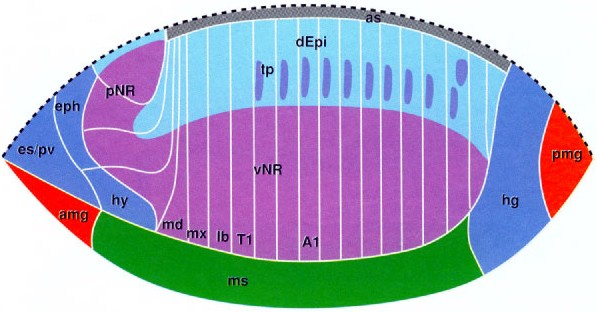
\includegraphics[width=0.45\textwidth]{./Images/blastoderm_fatemap_small.jpg}
  \centering
  \captionof{figure}{\textbf{Fate map of the \textit{Drosophila melanogaster} blastoderm}
  			The fate map is projected onto a planimetric reconstruction of the blastoderm. 
%  			The upper dashed line represents the dorsal midline and the lower margin represents the ventral midline.
  			A1 Abdominal segment 1; amg anterior midgut rudiment (endoderm); as amnioserosa; 
  			dEpi dorsal epidermis; eph epipharynx; es esophagus; hg hindgut; hy hypopharynx; 
  			lb labium; md mandible; ms mesoderm; mx maxilla;
  			pmg posterior midgut rudiment (endoderm); pNR procephalic neurogenic region; 
  			pv proventriculus; vNR ventral neurogenic region; T1 thoracic segment 1; 
  			tp tracheal placodes.
  			Diagram from \citet{Hartenstein1993}}
\label{fig:blastoderm_fatemap}
}
\par
%%%%%%%%%%%%%%%%%%%%%%%%%%%

\paragraph{Gene expression maps}

Techniques such as mRNA in situ hybridization allow to map gene expression patterns directly in the embryo. In situ hybridization is based on labelled probes that are complementary to the mRNA (or DNA) that is wanted to map \citep{Gall1969}. The probe accumulates then only where the mRNA of interest is found.
Another technique to map gene expression is the use of a reporter gene. A reporter gene, which codes for a protein that can be easily identified (like the green fluorescence protein or beta-galactosidase), is linked to the regulatory region of the gene of interest so the reporter gene is going to be expressed where the gene of interest is expressed.
Gene expression maps can also be used to create (or refine) fate maps \citep{gilbert2007fatemap}. 
For example, if a gene is know to be expressed only in mesoderm precursors, mapping their gene expression in the early embryo will reveal where such mesodermal precursors are located.

%Taking advantage of recent high-throughput methods of in situ hybridization \citep{Tomancak2002,Weiszmann2009}, the expression pattern of thousands of genes through \textit{Drosophila} embryogenesis have been systematically determined \citep{Tomancak2002,Tomancak2007,Hammonds2013}, and publicly available databases have been developed \citep{Tomancak2002,Kumar2011} so any researcher can see where and when a gene is expressed in the embryo.
%These databases are suitable for computational image analysis, as the protocols used to produce the images are standardized \citep{Tomancak2002} and the images can be aligned to an anatomical view (e.g., dorsal, lateral) \citep{Kumar2011}.
%With the expression patterns of thousands of genes, gene expression maps can be made using clustering techniques, showing regions where the expression of genes is more similar.
%Frise and collaborators made such analysis, processing thousands of in situ images of the blastoderm embryo and projected them into a virtual representation of the embryo made of ca. 300 triangles \citep{Frise2010}. 
%After clustering the triangles based on their expression similarity, they produce a co-expression map that resembled the fate map shown in Figure \ref{fig:blastoderm_fatemap}.

Importantly, fate maps (done by lineage tracking, histological or ablation methods) and gene expression maps do not necessarily have to coincide totally. Fate maps inform about which cells in the early embryo will give rise to different cell types or tissues, even when at such early stage the cells can be genetically equivalent.

\end{mdframed}
%%%%%%%%%%%%%%%%%%%%%%%%%%%%%%%%%%%%%%%%%%%%%%%%%%%%%%%%%%%%%%%%%%%%%%%%%%%%%%%%%%%


\subsection{Gene expression databases of \textit{D. melanogaster}}
\label{Intro_BDGP}

\subsubsection{Berkeley Drosophila Genome Project}
	\nomenclature{BDGP}{Berkeley Drosophila Genome Project}

The Berkeley Drosophila Genome Project (BDGP) is actually comprised of many projects, whose goals include 1) to complete the high quality sequence of the euchromatic genome of \textit{Drosophila melanogaster} and to generate and maintain biological annotations of this sequence; 2) to produce gene disruptions using P element-mediated mutagenesis; 3) to develop informatics tools that support the experimental process and identify features of DNA sequence; and 4) to characterize the sequence and spatial and temporal expression of cDNAs.

The BDGP insitu project has produced a high-throughput database of mRNA expression in different embryonic stages of \textit{D. melanogaster}, that can be used to complement and extend microarrays or RNAseq analyses \citep{Tomancak2002}. 
BDGP divides the first 16 stages of embryogenesis into six stage ranges (stages 1-3, 4-6, 7-8, 9-10, 11-12 and 13-16).

A brief description of the hybridization protocol follows, for details see \citep{Tomancak2002}.
For the hybridization, they used a set of cDNA clones from the Drosophila Gene Collection \citep{Stapleton2002}, to produce a digoxigenin-labeled antisense RNA probe \citep{Tomancak2002}.
Hybridization is carried out in fixed Drosophila embryos in 96-well plates. Successful hybridization plates are mounted on slides to document the expression pattern of each gene with high-resolution digital photographs. Then each image is assigned to one of six developmental stage ranges \citep{Weiszmann2009a}.
%
Finally, images and annotation data are stored in a modified version of Gene Ontology database. The entire dataset is available to browse or can be download from its webpage (http://insitu.fruitfly.org/cgi-bin/ex/insitu.pl).

%Taking advantage of recent high-throughput methods of in situ hybridization \citep{Tomancak2002,Weiszmann2009}, the expression pattern of thousands of genes through \textit{Drosophila} embryogenesis have been systematically determined \citep{Tomancak2002,Tomancak2007,Hammonds2013}, and publicly available databases have been developed \citep{Tomancak2002,Kumar2011} so any researcher can see where and when a gene is expressed in the embryo.
Databases like BDGP are suitable for computational image analysis, as the protocols used to produce the images are standardized \citep{Tomancak2002} and the images can be aligned to an anatomical view (e.g., dorsal, lateral) \citep{Kumar2011}.
An example of the power of using a computational image analysis approach is the work of Frise and collaborators.
\citet{Frise2010} analysed the spatial expression pattern of 1800 genes (from the BDGP database) in the blastoderm stage of \textit{Drosophila}, projecting them into a virtual representation of the embryo made of ca. 300 triangles.
After clustering the triangles based on their expression similarity, they produced a co-expression map that resembled the fate map shown in Figure \ref{fig:blastoderm_fatemap} (see Box 1 for a brief discussion of the relation between fate map and expression map).

%In here I used data from the BDGP insitu project whether by directly downloading data from their webpage (e.g., gene expression annotation data) or indirectly from the FlyExpress database (see next section). 

\subsubsection{Flyexpress}

The FlyExpress database (http://www.flyexpress.net/) contains a digitalized library of computationally filtered and standardized images from the high-throughput databases of mRNA expression Fly-FISH and BDGP, and from and peer-reviewed publications. It contains an image-matching search engine that can be used to search for many genes with similar or overlapping patterns of expression in the developing embryo.

The high-throughput databases from which FlyExpress extracts and computationally filter gene expression data differ in the hybridization protocol they use, the number of stages and the staging system, making direct comparisons between them difficult.
In contrast with the BDGP database (described in the previous subsection), Fly-FISH uses fluorescence in-situ hybridization probes \citep{Lecuyer2007} a 17-stage system (compared to a 16-stage system in BDGP) and five stage ranges (compared to six in BDGP).
%These databases also differ in the number of stages and the staging system, making comparisons between them difficult.
FlyExpress uses a semi-automated pipeline to standardize and align embryos, separating the multi- embryo images of BDGP into single images and discarding partial embryo images \citep{Konikoff2012}. 
After that, images are assigned to one of three an anatomical views: dorsal, ventral or lateral. Therefore, the expression pattern of a gene in a specific stage and view could be represented in FlyExpress by more than one in-situ image in more than one anatomical view.


In this work, from the images available in FlyExpress, I downloaded only those from BDGP, since BDGP uses more stage ranges than FlyFISH and these represent better the whole embryogenesis of \textit{D. melanogaster}. In the Fly-FISH database is focused specially in the early stages, as the last eight developmental stages are contained in one stage range (stages 10-17).
I used the FlyExpress database, instead of the BDGP directly, because the standardization protocol used by FlyExpress produces images with embryos in the same orientation and with a cleared background that are more suitable for image computational analysis.

%In addition to the methods, these databases differ in the number of stages and the staging system, making comparisons between them difficult. We used only the images coming from BDGP, since these expand over more developmental stages than the Fly-FISH database.

%	\clearpage
\section{The Hourglass model in \textit{Drosophila} }
	

\subsubsection{Adaptation in the embryo}

Usually, the study of adaptation
- general considerations of adaptation in the embryo

- example from marine animals

- Whyte

- entrenchment

- adaptive changes that influence adult/larva characters

- measurements of adaptation in the embryo in drosophila

- heatshock, developmental time, Dn/Ds.. etc.


\subsubsection{Hourglass model}

As we described in section X, von Baer stated in his "laws" that within a group of animals the general characteristics appear earlier in development, while the most special appear in late development \citep{vonBaer1828uber}.
This would lead to low morphogical variation at early development, gradually increasing as development proceeds.

Other authors \citep{Medawar1954,Slack1993,Duboule1994,Raff1996} proposed an alternative pattern in which there is great variation in early and late development, while the mid-development would show less variation.
The less variable (or more conserved) stage in mid development has been called the "phylotypic stage" or "phylotypic period".


although he recognized that the early stages were different (Gilbert 2010)

the hourglass model, proposed by (REFs)

mid-development conserved

natural selection?

Hox exagerations

With molecular evolution methods (see Subsec X), 


%	\clearpage
\section{Ciona}
	
	The ascidian \textit{Ciona intestinalis}, a marine invertebrate animal, has a long history in developmental biology and evolutionary biology. 
	Darwin highlighted the importance of the ascidians due to their close phylogenetic relationship to the vertebrates \citep{Darwin20009}. Although their adult form is a sessile filter feeder, its tadpole larva has characteristic features of the chordate group: a dorsal neural tube, a notochord surrounded by muscle and a ventral endodermal strand \cite{Satoh2003}. Also, it provided one of the first evidences of localized determinants of cell specification \citep{Conklin1905}.
	
	Some features of \textit{C. intestinalis} development that attracted the attention of developmental biologists more than a century ago included: the rapid embryonic development (it takes less than 20 hours from the fertilized egg to the larva), its invariant cell lineage and similitude between the ascidian larva and the vertebrate tadpole \citep{kowalewski1866entwicklungsgeschichte,chabry1887contribution}.
	More recently, the almost transparent body, which facilitate many genetic techniques, and the sequencing of the \textit{C. intestinalis} genome \citep{Dehal2002} are partly responsible for the re-emergence of \textit{C. intestinalis} as model organism in developmental biology \citep{Levin2012}.
	
Relevant efforts have been made to describe the spatial expression patterns of individual genes (REF).The spatial expression patterns of  >1,000 cDNA clones have been described using whole-mount in situ hybridization techniques at different developmental stages \citep{Imai2004}. Importantly, the developmental stages included cover a wide temporal range, e.g., blastula, gastrula and tapole stages \citep{Satou2005}.
	 Taking advantage of the ascidian invariant cleavage pattern and well described lineage analysis \citep{Conklin1905,Nishida1987}, the spatial expression of many genes have been described at the single cell level up to the early gastrula stage (REF), making this an invaluable resource to investigate the spatio-temporal dynamics of gene expression.



%	The \textit{C. intestinalis} genome is only 160Mb and contains ~16,000 genes, a gene number similar to the invertebrate \textit{D. melanogaster} genome and only is half of the genes found in some vertebrates (REF).
%	This low number of genes (compared to vertebrates) can be explained by the finding that many gene families or subfamilies have only one representative in \textit{C. intestinalis} \citep{Dehal2002}.

\subsection{\textit{Ciona intestinalis} life cycle}


\subsubsection{Developmental stages}

Ascidians, or tunicates (named after the "tunic" or thick cover in the adult form), are sessile animals that  attach to rocks and shells and filter plankton and other nutrients from seawater \citep{satoh2014developmental}.
During embryogenesis, ascidians show morphogenetic movements during gastrulation and neurulation similar to vertebrates and both share common genetic regulators of cell specification \citep{Satoh2003}.

As noted above, its larval form resembles a vertebrate tadpole.


Quick intro of developmental stages at 18$^\circ$C, based on \citep{Hotta2007}.

%%%%%%%%%%%%%%%%%%%%%%%%%%%%%%%%%%%%%%%%%%%%%%%%%%%%%%%%%%%%%%%%%%%%%%%%%%%%%%%%%%%%%
\label{Table_Ciona}
\begin{sidewaystable}
    \centering

\caption*{\textbf{Table 2. Embryonic stages of \textit{C. intestinalis} and main morphological characteristics (based on \citealp{Hotta2007}) }}
\begin{tabular}{|c|p{3cm}|p{3cm}|p{10cm}|}
\hline
\textbf{Stage}&\textbf{Description}&\textbf{Time after fertilization}& \textbf{Morphological characteristics} \\
\hline
\textbf{1}	& \textbf{Zygote}		& 0min to 55min 	&	From the fertilisation event up to the end of the first mitotic cycle \\
%
\textbf{2-5}	& \textbf{Early cleavage}& 55min to 3h	& Five mitotic divisions, until the 32-cell stage. First and second cleavages separate the left and right halves, and the anterior and posterior halves, respectively.  
%Asymmetric division of B5.2 due to the action of the centrosome atracting body (CAB), leads to a small posterior B6.3 cell. 
\\
%
\textbf{6-9}	& \textbf{Late cleavage}& 3h to 4.5h	& Very small B7.6 cell pair in the posterior end. Asymmetric divisions in the vegetal hemisphere. Embryo flattens on its vegetal side. Vegetal cells take a columnar shape\\
%
\textbf{10-13}	& \textbf{Gastrula}	& 1.5h to 6.3h	& Invagination and migration of endodermal and mesodermal cells inside the embryo. At the early gastrula, the vegetal side of the embryo takes a horseshoe shape. Embryo starts elongating anteriorly \\
%
\textbf{14-16}	& \textbf{Neurula}	& 6.3h to 8.5h	& The embryo, with an oval shape, continues elongating. Notochord precursors  intercalation and convergence. Neural tube formation and closure (starting from the posterior side)\\
%
\textbf{17-20}	& \textbf{Initial and early taibud}	& 8.5h to 10h	& Clear separation between trunk and tail. Neuropore closure. Tail starts bending \\
%
\textbf{21-22}	& \textbf{Mid tailbud}	& 10h to 11.9h	& Intercalation of the notochord cells is completed. The tail bends ventrally so the embryo adopts a half-circle shape. Length of the tail twice as long as the trunk	\\
%
\textbf{23-25}	& \textbf{Late tailbud}	& 11.9h to 17.5h 	& Pigmentation of the otolith can be observed. Palps formation. Vacuolization of notochord cells. The tail is bent dorsally   \\
%
\textbf{26}		& \textbf{Hatching}	& 17.5h 	& The larva hatches. Head adopts an elongated rectangular shape \\

\hline
\end{tabular}
%\end{adjustwidth}
\end{sidewaystable}

\subsection{The ANISEED database}

The ANISEED database (2015 version) integrates expression data from large-scale in situ hybridization studies with embryo anatomical data of ascidians \citep{Tassy2010,Brozovic2016}. 
This database includes 27,707 \textit{Ciona intestinalis} gene expression profiles by in situ hybridisation for approximately 4500 genes acquired from more than 200 manually curated articles \citep{Brozovic2016}.

The expression data is represented using an ontology-based anatomic description of the embryos. The ANISEED database also includes expression data from the Ghost database in \textit{Ciona intestinalis} \citep{Satou2005}, which contains the spatial expression patterns of  >1,000 cDNA clones by whole-mount in situ hybridization at different developmental stages.
Taking advantage of the invariant ascidian cleavage pattern and well-described lineage analysis \citep{Conklin1905,Nishida1987} the cDNA spatial expression have been described at the single cell level up to the early gastrula stage \citep{Imai2004}.

The ANISEED database also includes biometry data (e.g., volume, surface/volume) and 3D embryo models (at a single-cell resolution) of ascidian embryos until the early gastrula \citep{Tassy2006}. Importantly, combining the gene expression and 3D embyo models at a single cell resolution it is possible to reconstruct the gene expression pattern in 3D, as I did here. 
As the ANISEED database do not contains 3D embryo models for tailbud stages, in order to do reconstruct the gene expression in 3D in these stages, I used a 3D model of \textit{C. intestinalis} mid tailbud anatomy at a single cell resolution \citep{Nakamura2012}(see methods and study II).

	\clearpage
%%%% -----------------------------------------------------------------
%%%% -----------------------------------------------------------------

\chapter{Aims of the study}

In this work, I have analysed publicly accessible spatio-temporal gene expression data of two model organisms, \textit{Drosophila melanogaster} and \textit{Ciona intestinalis}, together with population genomics data of \textit{D. melanogaster}.
Using a statistical approach, I address three questions:
%%%%%%%%%%%%%%%%%%%%%%%%%%%%%%%%%%%%%%%%%%%%%%%%%%%%%%%%%%%%%%%%%%%%%%%%%%
\begin{enumerate}
\item How do complexity and compartmentalization increase in the embryo during development?
\item Can adaptation be found in specific anatomical parts of the embryo or developmental stages? 
\item Is the Hourglass model (which states that there is less amount of inter-specific variation in mid-development; see section \ref{hourglass}) supported by evidence of natural selection at the DNA sequence level?
\end{enumerate}
%%%%%%%%%%%%%%%%%%%%%%%%%%%%%%%%%%%%%%%%%%%%%%%%%%%%%%%%%%%%%%%%%%%%%%%%%%

These questions have been selected for the great interest they have aroused in the scientific community since the early days of developmental and evolutionary biology.
%
The work presented here is based on and uses concepts from three main biology fields: 
developmental biology, evolutionary biology and population genetics.
Nowadays, the combination of these scientific fields constitute multiple research programmes. Modern evolutionary developmental biology (evo-devo) is the explicit combination of the first two fields.
	\nomenclature{evo-devo}{Evolutionary developmental biology}


%%%% -----------------------------------------------------------------
%%%% -----------------------------------------------------------------

\chapter{Material and Methods}
	\section{On the complexity measures used in this work}
	
In the following paragraphs I will describe the three measures of complexity I used in here: relative area/volume, disparity and roughness. I consider them complexity measures because they inform about specific features in embryonic development that are intuitively associated to the increasing complexity of the organism. The relative area/volume of expression relates to the notion of the progressive compartmentalization of the embryo, disparity informs about how the different parts of the embryo become more different (at the genetic level) from each other, and the roughness measure relates to the notion of genes being expressed in progressively more complex spatial expression patterns (as defined by the shape of the gene expression pattern).


\subsubsection{Compartmentalization}

As mentioned before, the process of embryo compartmentalization, or the subdivision of the embryo in different parts during development, is considered to be largely reflected in the expression of the genes in progressively smaller areas. Therefore, a good measure of compartmentalization would be to measure the relative area of expression of all genes during development.
Gene expression patterns are usually visualized as a 2D image, which reflects the distribution of a gene product from a specific anatomical view (e.g., lateral, dorsal).  More recently, methods like 3D imaging technique Optical Projection Tomography  \citep{Sharpe2003,Summerhurst2008} allow to record gene expression patterns in 3D.

In the case of 2D images, the measure of compartmentalization I use in here is the relative area of the expression of a gene divided by the area of the whole embryo (pixels with expression divided by all the pixels of the embryo image). I called this measure "relative area" which ranges from 0 (no expression) to 1 (ubiquitous expression). 
In the case of a gene expression in 3D, the compartmentalization measure becomes the relative volume of expression, which also ranges from 0 to 1 and is calculated as the volume of the cells/tissues with expression divided by the whole embryo volume.
Of course it could be said that the compartmentalization of an embryo should not only be reflected in the decrease of the relative area of expression of the genes during development, but also should be reflected in a greater proportion of genes expressed differentially in different parts of the embryo. To account for this, I used a "disparity" measure (explained below), that would be informative in the mean degree of dissimilarity between the different parts of the embryo.

\subsubsection{Disparity}

The disparity measure is related to  McShea's "number of part types" complexity measure. Ideally, the number of cell types, if this could be precisely known, would be a good measure of complexity during development. However, as mentioned before, there is no clear criteria to determine when (at the genetic level) a new cell type is formed during development.

%Usually, genetic markers are used to determine if a cell (or its descendants) can be considered a specific cell type. This could be the case of anterior or posterior compartment cells within \textit{D. melanogaster} para-segments. For example, the use of wingless (\textit{wg}) or sonic hedgehog (\textit{hh}) in situ hybridization can be used to define if a cell is part of the anterior or posterior compartment. It could be said, however, that the earliest presence of expression of these genes marks the \textit{fate} of the cell, more than the actual cell type. In fact, before the anterior and posterior segment compartments are completely defined, the expression level of these genes changes over time and form a positive feedback to stabilize each other expression. Therefore, a cell that early expresses \textit{wg} would not necessarily differentiate into a posterior compartment if its neighbour para-segment does not express \textit{hh} \citep{Bejsovec1991}.
 
Instead of trying to determine the number of cell types during development, I decided to quantify how different at the gene expression level are the cells or regions in the embryo. In \textit{D. melanogaster}, as it was not possible to have expression for each individual cell, I divided the 2D embryo in "regions" of approximately the same area using polar coordinates (Fig. \ref{fig:roughness_regions}A; see study I). 
In the case of \textit{C. intestinalis}, I used expression data at a single cell level for the early stages and at tissue level for the tailbud stages (see study II).

To quantify this, I decided to use pearson's correlation as similarity measure between cells/tissues or regions. With this method, the expression of all the genes available in two cells can be compared, giving a value of 1 if all genes have exactly the same expression (their expression is completely correlated), to -1 if all the genes show opposite gene expression (their expression is anti-correlated). 
An advantage of this method is the possibility to include the information of all available genes, diminishing a possible bias in the gene selection. 

The pearson's correlation matrix is a measure of gene expression similarity between genes. In here, I was interested on quantifying the difference (i.e., disparity) in gene expression between cells, not on their similarity. Therefore, the disparity between two cells becomes: disparity = 1 - pearson's similarity. The disparity measure ranges from 0 to 2, with a 0 value when the gene expression between cells is exactly the same.

%%%%%%%%%%%%%%%%%%%%%%%%%%%%%%%%%%%%%%%%%%%%%%%%%%%%%%%%%%%%%%%%%%%%%%%%%%%%%%%%%%%%%%
\begin{figure}[h]
  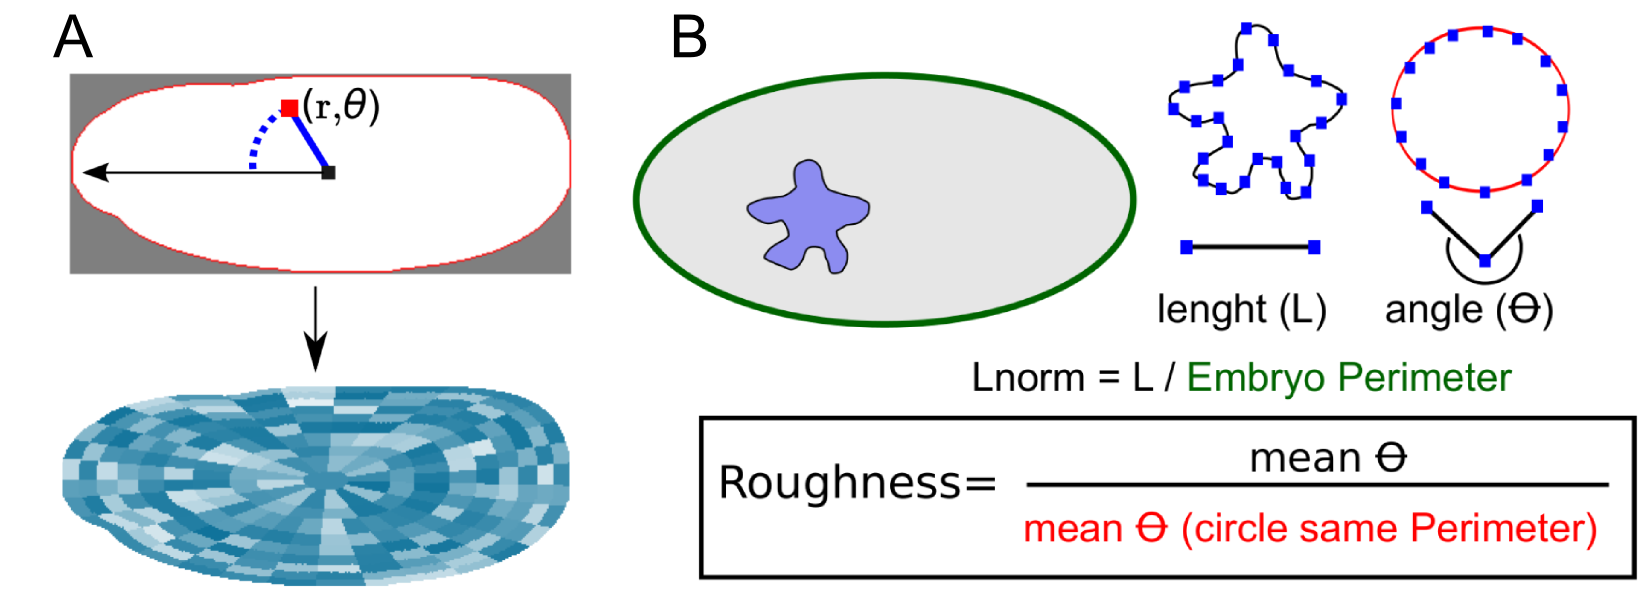
\includegraphics[width=0.85\textwidth]{./Images/roughness_regions.png}
  \centering
  \caption{\textbf{Polar regions and 2D roughness measure}. A) The embryo of each stage was divided in 257 regions using polar coordinates. The embryo for stage 11-12 is shown with the 257 regions in a random color. B) A schematic embryo (gray) with a gene expression pattern in blue. Roughness is the mean major angle ($\theta$) between each node (at every L length pixels in the contour) and its two immediate neighbours, normalized by the mean angle of a circle of the same perimeter.
   }
  \label{fig:roughness_regions}
\end{figure}
%%%%%%%%%%%%%%%%%%%%%%%%%%%%%%%%%%%%%%%%%%%%%%%%%%%%%%%%%%%%%%%%%%%%%%%%%%%%%%%%%%%%%

\paragraph{Synexpression Territories} 
Another advantage of using a pearson's correlation matrix, is the possibility of using a clustering algorithm (e.g., hierarchical clustering), for example, to find the main temporal patterns of gene expression in microarray analysis \citep{Eisen1998,Wen1998}. 
%Also, this method can be used to separate cell types based on the genetic differences between them \citep{gohlmann2009gene}.
\textbf{AQUI PONER LOS TERRITORIOS DE CIONA Y DROSOPHILA}


\subsubsection{Roughness}

The roughness measure analyses the complexity of the shape of a gene expression pattern. In the case of 2D images, the shape of the gene expression pattern is extracted as a closed outline formed by the boundaries of gene expression, while for 3D patterns, the shape of the expression pattern is the 3D external surface of the union of the cells that are expressing such gene.

Therefore, a gene expression pattern reflects necessarily the spatial distribution of the cells expressing such gene. When analysing and comparing the shape of diverse gene expression patterns, i.e., the cells/tissues with expression are different between genes, there is an obvious impossibility to determine landmark points (whether around a 2D outline or 3D surface) that would establish a clear one-to-one correspondence between them. This could be done in the case of comparing the expression pattern of a single gene at a specific developmental stage between different individuals.
Therefore, a landmark-free method (like outline methods for 2D or surface methods for 3D data) is best suited to deal with the type of data analysed in here.

There are practically no studies in the literature that have quantified and compared the shape of gene expression patterns in a systematic manner (one exception is the recent study of \citealp{Martinez-Abadias2016}). In here, I will consider that a gene expression pattern is complex if based on the curvature of its 2D contour or 3D surface.

\paragraph{2D Roughness}
For 2D gene expression patterns, I used a "roughness measure", that is similar to the shape function $\phi^{*}(l)$ used in eigenshape analyses \citep{Lohmann1983}, as it measures how much the curvature of a closed outline deviates from the angles of a circle of the same perimeter (Fig. \ref{fig:roughness_regions}B; see study I). 
To calculate the roughness of a expression pattern I first selected points in the contour every L (length) pixels. Then, vectors between each node and the two immediate neighbour nodes in the contour are calculated and the biggest angle formed between them is measured. The roughness value is then the mean angle normalized by the mean angle of a circle of the same perimeter.

I selected the roughness measure instead of some other measure outline based method like Fourier analysis because the roughness value gives an intuitive descriptor of complexity, i.e., a value of 1 would be a simple "circle-like" shape, and a value greater than 1 would mean a higher curvature of the outline. \citet{McLellan1998} compared various measures of spatial complexity applied to the outlines of the leaves of many tree species. They included a "margin roughness" measure that is very similar to the one I use here (the difference is that they does not normalize by the mean angle of the circle nor he uses different lengths of vectors) and found that there was no marked differences between the margin roughness and a Fourier analysis with up to 64 harmonics (both performed equally well).
%On the contrary, one advantage of the Fourier analysis would be that it is an information preserving algorithm \citep{Pavlidis1980} i.e., it is possible to reconstruct the shape after the analysis, a feature that was not considered relevant for this study. 
Other feature of the roughness measure is that allows to measure the complexity of shape at different spatial scales. Therefore, it can be tested not only if the complexity of the gene expression shape increases during development, also if this increase is the same at different spatial scales.

\paragraph{DNE}
In order to use a similar measure of curvature in 3D, I used the Dirichlet normal energy (DNE; described briefly in section \ref{DNE_explanation} which quantifies the deviation of a surface from being planar (Fig. \ref{fig:DNE}; see study II). 
Importantly, both measures are normalized to remove size and orientation effects.

%%%%%%%%%%%%%%%%%%%%%%%%%%%%%%%%%%%%%%%%%%%%%%%%%%%%%%%%%%%%%%%%%%%%%%%%%%%%%%%%%%%%%%
\begin{figure}[h]
  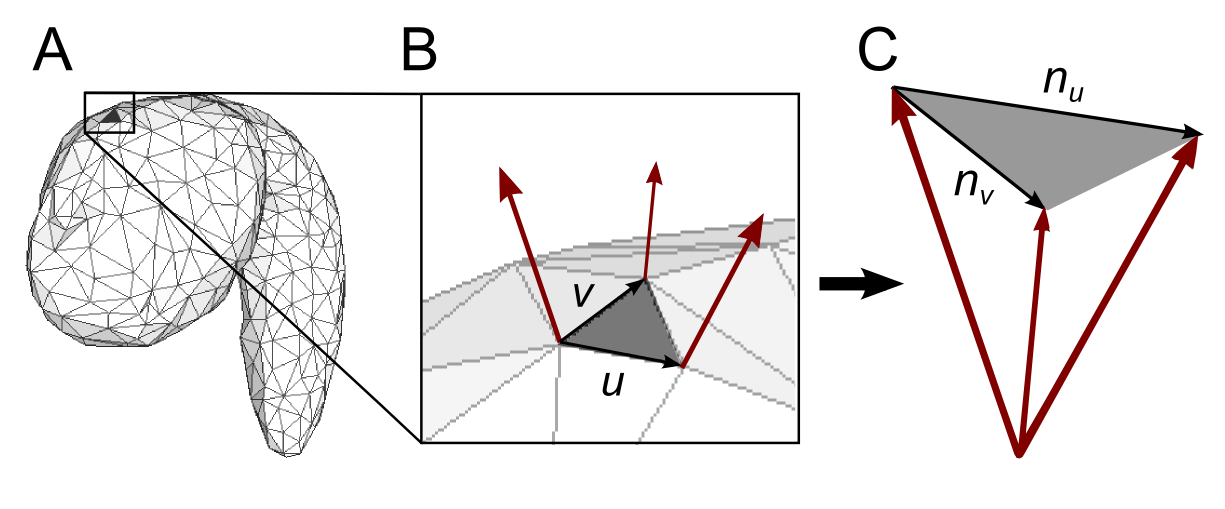
\includegraphics[width=0.7\textwidth]{./Images/DNE.png}
  \centering
  \caption{\textbf{Dirichlet Normal Energy (DNE).} A) A surface mesh representing a a mid-tailbud embryo in C. intestinalis. B) DNE calculates the energy value $e(p)$ of each polygon (like the one in grey) in the surface. The polygon is characterized by vectors $u$ and $v$, which represent the edges of the polygon. Then, normal unit vectors are estimated as the normalized average of normal vectors of the triangle faces adjacent to each vertex (red arrows). C) If vertex normals are translated to a common origin point, their end points form a polygon with edge vectors $nu$ and $nv$, which represent the spreading of $nu$ and $nv$. In a simplistic way, DNE can be defined as the spreading of $nu$ and $nv$ relative to the spreading of $u$ and $v$ \citep{Bunn2011,Winchester2016}. 
 }
  \label{fig:DNE}
\end{figure}
%%%%%%%%%%%%%%%%%%%%%%%%%%%%%%%%%%%%%%%%%%%%%%%%%%%%%%%%%%%%%%%%%%%%%%%%%%%%%%%%%%%%%

To calculate the DNE, I used the Morphotester software version 1.1.2 \citep{Winchester2016}
available in the webpage "http://morphotester.apotropa.com/". DNE was calculated using the "implicit
fair smooth" option of Morphotester, which reduces surface mesh noise which can disproportionately affect DNE values (Winchester, 2016). 

It is important to mention that the aim of this analysis is not to discern which mechanisms (e.g., cell-cell signalling or morphogenetic movements) are responsible for the changes in complexity of the shape of gene expression pattern, but to quantify how this happens during embryonic development.

\subsubsection{The relationship between these measures}

The three different measures of complexity are informative of different and independent aspects of complexity and are not necessarily correlated. 
For example, a decrease in the area/volume of gene expression should not necessarily mean an increase in disparity, as the genes that are reducing their expression area could be restricted to the same part of the developing embryo. 
Only in the case of an embryo with all genes showing ubiquitous expression, there is a clear relationship between disparity and relative area/volume, as the relative area of expression and disparity would be 0 and 1 respectively. If there are however, many genes expressed in only a part of the embryo, these measures are not necessarily correlated. 

This can be illustrated with a simple example shown in Fig. \ref{fig:measures_relations}, in which there are different alternative gene expression scenarios of an imaginary embryo with six cells. In each scenario, the embryo expresses four genes in different relative areas (i.e., in a different number of cells). The mean relative area is 0.5 for all scenarios, but the mean disparity varies in a two-fold manner. In the scenario that shows the largest disparity, each cell expresses a unique combination of genes, while the scenario with the lowest disparity, 4 of 6 cells do not have a unique expression profile.

The roughness and disparity independence can be easily exemplified in the case of a blastula. Blastula is the name to define the multicellular aggregate stage that results from the subdivision (cleavage) of the zygote. The blastula shape topology and geometry is usually simple \citep{Forgacs_Newman2005}, typically consisting of a ball of cells with an interior cavity (called "blastocoel"). If in a spheric blastula, composed of also spheric cells (like that of a sea urchin) a large proportion of genes would be expressed ubiquitously and a small proportion of genes would be expressed in single cells, both roughness and disparity would be relatively low.
However in the case of a large proportion of genes expressed in different single cells, and a low proportion of genes expressed ubiquitously, the disparity would be high, but the roughness would be very similar than in the previous case. This would be because the roughness quantifies the shape of the expression pattern, irrespective to size. Therefore the roughness of a gene expression in a single spheric cell would be practically the same that the roughness of a gene expression in the whole spheric embryo.

The independence of the roughness measure with the size of the gene expression (i.e., relative area/expression) comes from the roughness normalization. The normalization of the 2D roughness consists of dividing the mean angle of a gene expression pattern by the mean angle of a circle with the same perimeter, and in the case of 3D roughness (i.e., DNE) it consists on transforming the 3D expression surface into a polygonal surface mesh with a determined number of polygons. 
%Therefore, these three measures of complexity should be informative on how genes become restricted to smaller regions (relative area/volume), how different is the gene expression of the different parts of the embryo (disparity) and how complex is the gene expression pattern shape (roughness) at different times of development.


%%%%%%%%%%%%%%%%%%%%%%%%%%%%%%%%%%%%%%%%%%%%%%%%%%%%%%%%%%%%%%%%%%%%%%%%%%%%%%%%%%%%%%
\begin{figure}[h]
  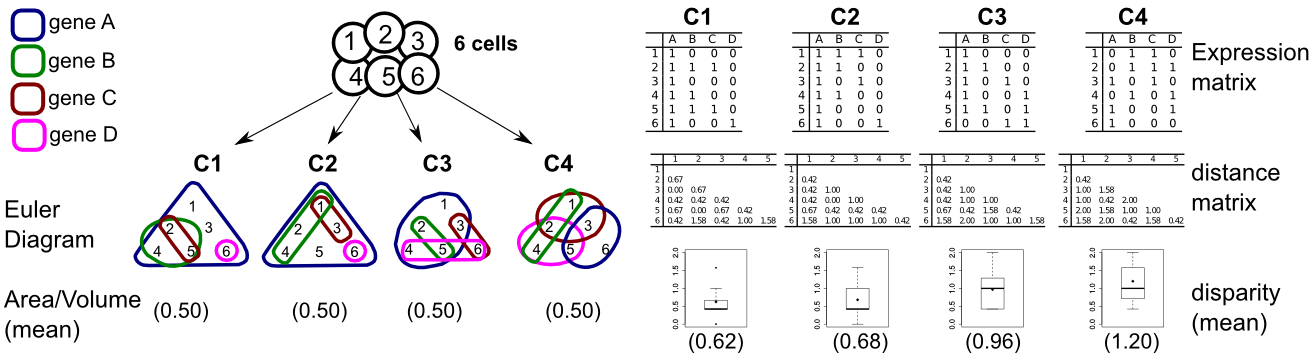
\includegraphics[width=0.95\textwidth]{./Images/measures_relations.png}
  \centering
  \caption{\textbf{Relation between area/volume of expression and disparity measures.} An embryo of six cells (top left) is shown expressing four different gene expression combinations (C1, C2, C3 and C4) of four genes (A, B, C and D). All combinations have a mean relative area/volume of 0.5. Each gene expression configuration is represented as an Euler diagram (representing the subset of the cells in which it is expressed in a color code shown at the top left) and as binary expression matrix (top right). The pairwise distance between the cells, calculated as 1-(pearson's correlation), is shown as a matrix. At the bottom right, a distribution plot of the pairwise distances of each combination and the mean disparity are shown below in parenthesis.
 }
  \label{fig:measures_relations}
\end{figure}
%%%%%%%%%%%%%%%%%%%%%%%%%%%%%%%%%%%%%%%%%%%%%%%%%%%%%%%%%%%%%%%%%%%%%%%%%%%%%%%%%%%%%


	\section{Data mining and handling}
	The work presented here is based on the analysis of publicly available data contained in many databases, shortly introduced in the Review of the Literature section. In the next paragraphs I will describe how the data used in here was acquired and processed, for the details, see the corresponding study.

\subsubsection{In situ Hybridization data}

\paragraph{\textit{D. melanogaster} (study I and III)}

Images were downloaded from the FlyExpress Database version 5.1 \citep{Kumar2011} on February 2013. Only genes with laterally oriented images for the six stages used in BDGP \citep{Tomancak2002} were considered.

Images were systematically retrieved and resized to 320 x 128 pixels (as in \citealp{Konikoff2012}) with ad-hoc Perl scripts.
%
The gene expression pattern was obtained using an adaptive threshold based on the mean and variance of a grey-scale version of each image. Three different threshold were used, resulting in three different filtered gene expression patterns of each original in situ image. I visually selected the image that resembled the most to the original gene expression pattern. Genes with ubiquitous expression in stages 1-3 and 4-6 were considered as entirely black images.

To correct for small variation in the shape of the embryos I adjusted each embryo to an stage ideal embryo shape, with an algorithm I made to morphometrically deform the real embryo contour of each image to the corresponding stage ideal shape.
Finally I applied a "smoothing filter" to produce a smooth expression pattern and eliminate isolated white/black pixels. I also manually filtered images from the literature or directly from BDGP of Transcription Factors or Growth Factor genes that did not have information in FlyExpress. These manually filtered images were also morphometrically deformed with the algorithm mentioned above. The resulting dataset contained 1218 genes with expression information in the six stages used in BDGP.

In addition to the whole-mount in situ RNA-hybridization images, the BDGP database contains, for each gene, the list of the embryonic anatomical structures in which such gene is expressed \citep{Tomancak2007}. Each gene expression is described by one or several of those of anatomical terms by an expert. 
This information was retrieved from the BDGP downloads page (http://insitu.fruitfly.org/insitu/html/downloads.html/), which contains the annotations of almost 8,000 genes. We removed genes with only "no staining" as anatomical term, leaving a total of 5762 genes.

\paragraph{\textit{C. intestinalis} (study II)}

I downloaded the in situ hybridization data (ish.zip file) from the download section of the ANISEED database on 28th of December 2015. 
The expression data for the first three stages is at the cell level, while in the tailbud stages is at the tissues or specific regions of the embryo level. 
I extracted the information of the 32 cells, 64 cells, 112 cells, early tailbud, mid tailbud and late tailbud stages. Only expression data from experiments reported to have Wild type phenotype, "public" publication status, with in situ hybridization as experiment design and whose probe was assigned to a Kyoto Hoya (KH) \citep{Satou2008} gene model.
I excluded data from experiments whose image characterization was reported as "not sure" or too broadly as "part of whole embryo".

The number of genes analyzed is n=745 for the 32-cell stage, n=758 for the 64-cell stage, n=809 for the 112-cell stage, n=1082 for the early tailbud, 1092 for the mid tailbud and 887 for the late tailbud. 

\subsection{Transcriptomics ans population genomic data}

\paragraph{modENCODE (study III and IV)}

Gene expression levels in reads per kilobase per million mapped reads (RPKM) units for 30 developmental stages were retrieved from \citet{Gelbart2013}, who analyzed RNA-seq throughput data from the modENCODE project \citep{Graveley2011}.

For using RNA-seq data to compare expression between samples, a normalization step was performed to adjust for varying sequencing depths and other potential technical effects across replicates (see study III)

\paragraph{DGRP (study II and IV)}

The population genomic data comes from 168 inbred lines of \textit{D. melanogaster} sequenced in the Freeze 1.0 of the Drosophila Genetic Reference Panel (DGRP) project \citep{Mackay2012}. The DGRP population was created collecting gravid females from a single population of Raleigh, North Carolina (USA), and following the full-sibling inbreeding approach during 20 generations to obtain full homozygous individuals. 
DGRP lines showing high values of residual heterozygosity (>9\%) that were observed to be associated with large polymorphic inversions \citep{Huang2014} were not included.

Due to requirements of the software used to estimate the rate of adaptive substitution, 
the original data of 168 lines set was reduced to 128 isogenic lines by randomly sampling the polymorphisms at each site without replacement. Finally, residual heterozygous sites and sites with no quality value were excluded from the analysis.







	\section{Estimating adaptation}
	
To estimate adaptation during \textit{D. melanogaster} embryogenesis, the DFE-alpha method and the software were used (see section \ref{alpha}; \citealp{Eyre-Walker2009}), which infer adaptation combining polymorphism and divergence data.

The DFE-alpha software (DFE-alpha, Eyre-Walker and Keightley 2009 ;see below) requires that all sites to have been sampled in the same number of chromosomes. Therefore, the original DGRP dataset was reduced to from 168 to 128 isogenic lines by randomly sampling the polymorphisms at each site without replacement. Residual heterozygous sites and sites with no quality value were excluded from the analysis.
%
This software estimate several parameters (e.g., $\alpha$ and $\omega_{\alpha}$) from a set of genes as estimates based on single genes can be affected by the lack of segregating (divergent) sites. Therefore, in each analysis a group of genes was randomly sampled (bootstrap with replacement) (see studies III and IV). 
As neutral reference the positions 8-30 of short introns ($\leq$ 65 bp) were used (as in \citealp{Heyn2014}). For validation, 4-fold degenerate sites were also used.

The release 5 of the Berkeley Drosophila Genome Project was used as the reference genome (http://www.fruitfly.org/sequence/release5genomic.shtml/). The divergence statistics were estimated from a multiple genomic alignment between DGRP lines and \textit{D. yakuba} BDGP 5 coordinates (from http://popdrowser.uab.cat; \citealp{Ramia2012}).
The number of sites and substitutions and the folded site frequency spectrum (SFS) were computed using an ad hoc Perl script.

Ortholog genes between \textit{D. yakuba} and \textit{D. melanogaster} were obtained from FlyBase (http://flybase.org/). \textit{D. yakuba} was used as outgroup species as, due to the time since their divergence, there is less chance of ancestral polymorphism contributing to divergence, diminishing the effect of low divergence affecting the estimates of adaptive evolution \citep{Keightley2012}.

%\input{./Parts/Methods}
\clearpage

%%%% -----------------------------------------------------------------
%%%% -----------------------------------------------------------------
	
\chapter{Results and Discussion}

%\section{Complexity and compartmentalization in \textit{Drosophila}}
%	\subsection{High compartmentalization and disparity around gastrulation}
%objective
I estimated the degree of compartmentalization calculating the relative area of expression of hundreds of genes during development.
My intention here was not to focus on individual genes, but to get a global overview of the embryo compartmentalization and differentiation processes.

%results
The results showed a non-linear decrease in the mean relative area of expression (an inverted saturation curve), with the major decrease occurring at very early development, from maternal to early gastrula stage (Fig. \ref{fig:Art-I-3measures}).
Practically half of the genes in follows this decrease pattern: 46\% of the genes were characterized as having a non-linear decrease in their relative area.
The results show that the disparity increases non-linearly, again with the major change in the early stages.
%
It is important to notice that these should not be necessarily the case, as the disparity relates to how different genetically are the different regions of the embryo in different stages, so it could be that between two stages the relative area of expression decreases but not the disparity if the genes are expressed in the same part of the embryo.

%discussion

These results are consistent with the hypothesis that the \textit{Drosophila} embryo becomes compartmentalized in a progressively more fine-grained manner over developmental time. 
More importantly, they show that this process happens quite early, i.e., around gastrulation.
This is, most genes start being expressed in broad areas of the embryo and over time their expression becomes progressively restricted into smaller and smaller spatial domains.

This earlier compartmentalization probably is due to \textit{Drosophila}'s derived early development, namely, the syncytial blastoderm. During this stage, approximately 4,000 cell nuclei can `communicate' with each other only by TFs \citep{Jaeger2011}. The direct cross regulation of gene expression facilitates a rapid and highly dynamic process which seems to be responsible for the early spatial restriction of a great proportion of developmental genes.

%%%%%%%%%%%%%%%%%%%%%%%%%%%%%%%%%%%%%%%%%%%%%%%%%%%%%%%%%%%%%%%%%%%%%%%%%%%%%%%%%%%%% 
\begin{figure}[h]
  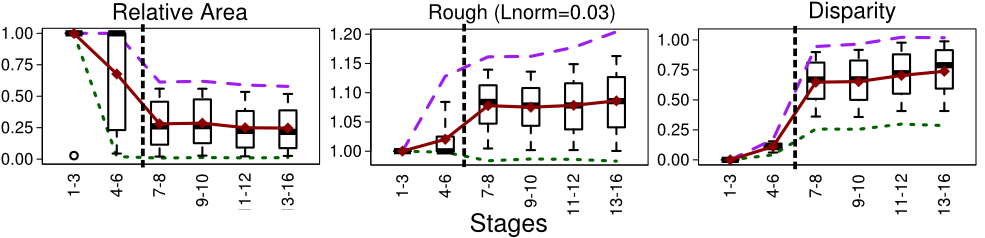
\includegraphics[width=\textwidth]{./Images/Art-I/3_measures.png}
  \centering
  \caption{Distribution plot of the relative area of expression (left), roughness (center) and disparity (right) for all genes in each stage. Diamonds represent the mean, boxes the IQR. Whiskers 10 and 90 percentiles. Dashed line represents the max values and dotted line the min values (mean of the last and first decile, respectively). Stages on the x-axis, vertical dashed line represents gastrulation entry.}
  \label{fig:Art-I-3measures}
\end{figure}
%%%%%%%%%%%%%%%%%%%%%%%%%%%%%%%%%%%%%%%%%%%%%%%%%%%%%%%%%%%%%%%%%%%%%%%%%%%%%%%%%%%%% 

\subsection{The leading role of TFs and GFs}

%objective
Then, I wanted the test if the hypothesis transcription factors (TFs) and growth factors (GFs) have a a leading role in pattern formation and compartmentalization.
%results 1
The TFs (GO:0003700) and GFs (GO:0008083) showed smaller relative area of expression that the rest of genes in the blastoderm stage (Fig. \ref{fig:Art-I-3measures}).
	\nomenclature{GF}{Growth Factor}
	\nomenclature{KW}{Kruskal-Wallis test}
%
The TFs are also expressed in smaller areas than the rest of the genes in all subsequent stages, while the GFs are expressed in smaller areas at the blastoderm (stage 4-6) and extended germ band stages (stage 9-10 and 11-12) (I, Fig.4).

%discussion 1
These results are complementary to the study done by \citet{Hammonds2013}, who made an extensive analysis of TFs expression using the BDGP database, using manual annotation of gene expression based on an anatomical controlled vocabulary and classifying every gene as ubiquitous, patterned, ubiquitous-patterned, or maternal. 
They found that the fraction of TFs expressed in a restricted pattern (assigned to a tissue) was higher, when compared to other genes, in all zygotic stages with the exception of the stage 13-16. 

The results I show for stages 4-6, 7-8, 9-10 and 11-12 are consistent with Hammonds et al., as the higher proportion of the TF genes showing a restricted or tissue-specific expression pattern would imply that TFs are expressed in smaller areas in the embryo. For the 13-16 stage, contrary to these authors, I showed that the TFs are highly compartmentalized. This might indicate a limitation of the annotation method used by Hammonds et al., to capture the high spatial compartmentalization of the TFs in this stage.

In general, these results support the hypothesis of the leading role of TFs and GFs in driving pattern formation and compartmentalization in the early embryo.

%results & discusion 2
In the blastoderm stage the disparity of the regions based only on the TFs is much greater than the one based on all the genes ((KW pvalue $<0.001$; Fig. \ref{fig:Art-I-3measures}) indicating that these genes account for a large portion of the diversity of gene expression patterns.

In general, the fact that TF genes have lower relative area (i.e., are more compartmentalized) than the rest of the genes, especially in the stage before entering gastrulation, is consistent with the leading role of these genes in driving pattern formation and the resulting compartmentalization of the embryo.

%%%%%%%%%%%%%%%%%%%%%%%%%%%%%%%%%%%%%%%%%%%%%%%%%%%%%%%%%%%%%%%%%%%%%%%%%%%%%%%%%%%%% 
\subsection{Roughness increases non-linearly}
%objective
The roughness measure informs about the overall imbrication or convolution of the shape of a gene expression contour at different spatial scales, relative to a circular shape.
%results
Our results (Fig. \ref{fig:Art-I-3measures}) show that roughness increases in a non-linear way during development, and that the major increase is in the transition from the blastoderm to the early gastrula.
The maximal values (mean of the last decile) increase initially in the pre-gastrula, reach a stationary phase at mid-embryogenesis and finally increase in the last stages. 
As I mentioned in the literature review (section X), the maximal values are informative about the overall morphological spatial complexity of the embryo in a given stage.

When comparing roughness at different spatial scales (I, Methods), I found that in the last three stages the roughness values are significantly higher at smaller spatial scales is significantly higher that at the higher spatial scales.(Fig. S2 in article I). 
%discussion
This suggests that complexity may be increasing not only through all the development but also that it does at finer spatial scales over time.


%%%%%%%%%%%%%%%%%%%%%%%%%%%%%%%%%%%%%%%%%%%%%%%%%%%%%%%%%%%%%%%%%%%%%%%%%%%%%%%%%%%%% 
\subsection{Main spatio-temporal profiles of gene expression}
%objective
I performed a time series cluster analysis \citep{Ernst2006} using the relative area of expression in order to know which were the most common spatio-temporal profiles (I, Fig. 5).
%results
I found eight main spatio-temporal profiles, the most common following the global profile of non-linear decrease in the first stages (I, Fig 5)

Among the rest of profiles, I found both linear increase and decrease profiles and a `hill-like' profile (initial increase and further decrease with the higher values at stage 7-8)
%
The linear decrease profile (n=167 genes) was enriched with `mitotic cell cycle' (GO:0000278), `RNA processing' (GO:0006396) and `chromatin modification' (GO:0016568) GOterm genes, highlighting biological processes that first are present in the whole embryo and become more and more restricted in space as development proceeds.
%discussion
The `mitotic cell cycle' term, for example, most likely relates to the fast mitotic cycles in the earliest embryo. During stage 1-3 nine fast and synchronic mitotic divisions take place in the entire embryo, then in stage 4-6 mitotic divisions 10-13 occur more slowly, almost synchronically. The 14th cycle, zygotically controlled, is long and of different durations in the embryo.

With a temporal co-expression cluster analysis using microarray data through the life cycle of \textit{D. melanogaster}, \citet{Arbeitman2002} found that most cell cycle genes were expressed at high levels during the first 12h, but only a few are expressed at high level thereafter.
My analysis is consistent with this, as I found that the profile of linear decrease (I, Fig. 5A) is enriched with such genes. In this sense, this study is complementary to Arbeitman et al., and adds the spatial dimension to their temporal expression profiles.


%%%%%%%%%%%%%%%%%%%%%%%%%%%%%%%%%%%%%%%%%%%%%%%%%%%%%%%%%%%%%%%%%%%%%%%%%%%%%%%%%%%%% 
\subsection{Gene synexpression territories in the embryo}
%objective
Finally, using a clustering algorithm, I made a dendrogram representing the relative degrees of similarities between all regions of all the stages at the same time (Fig. \ref{fig:Art-I-territories} A).
After cutting the dendrogram at a certain level and choosing only territories with at least 50 genes expressed with a minimum specificity (see methods in I for a detailed description), I ended up with 30 clusters (Fig. \ref{fig:Art-I-territories} B), which I will call `synexpression territories' (ST) from now on.
	\nomenclature{ST}{Synexpression territories}
I grouped the STs in eight `meta-territories' to analyse how the different STs relate between them.

%results
The results show that stages 1-3 and 4-6 each one form a ST. If a cut-off is selected so that stage 4-6 is divided in four sub-territories (I,Fig. S3) the embryo splits in four parts: anterior, posterior, dorsal and ventral.
This correspond to a nearly Cartesian system one could expect from the two signalling systems known in the earliest patterning in \textit{Drosophila} (the A/V and D/V signalling cascades; \citep{Gilbert2014}).
%
The STs seem to coincide with the known embryo fatemap (see Fig. \ref{fig:Art-I-territories} D; \citealp{Hartenstein1993}) and many of them are enriched with GOterms that coincide with their expected fate.
For example, in stage 7-8 (just after gastrulation) there is a ST that corresponds spatially with the germband and is enriched with mesodermal GOterms (Fig. Fig. \ref{fig:Art-I-territories} C).

There are two meta-territories that appear in the last stage (light blue and green, Fig. \ref{fig:Art-I-territories} C), which suggests that the tissues/organs related to those STs differentiate quite late.
%
%% discussion
One is enriched with terms related to epidermis such as cuticle development (`chitin catabolic process' [GO:0006032] and `cuticle development' [GO:0042335] synexpression territories 33 and 38), which coincides with cuticle deposition by epithelial cells during stage 16 \citep{Ostrowski2002}.
%
The other corresponds spatially with the CNS of the embryo and is indeed enriched with CNS GO-terms
The CNS territory is enriched with GOterms like `dendrite morphogenesis' (GO:0048813) and `axon guidance' (GO:0007411). 
	\nomenclature{CNS}{Central Nervous System}

\begin{figure}[h]
  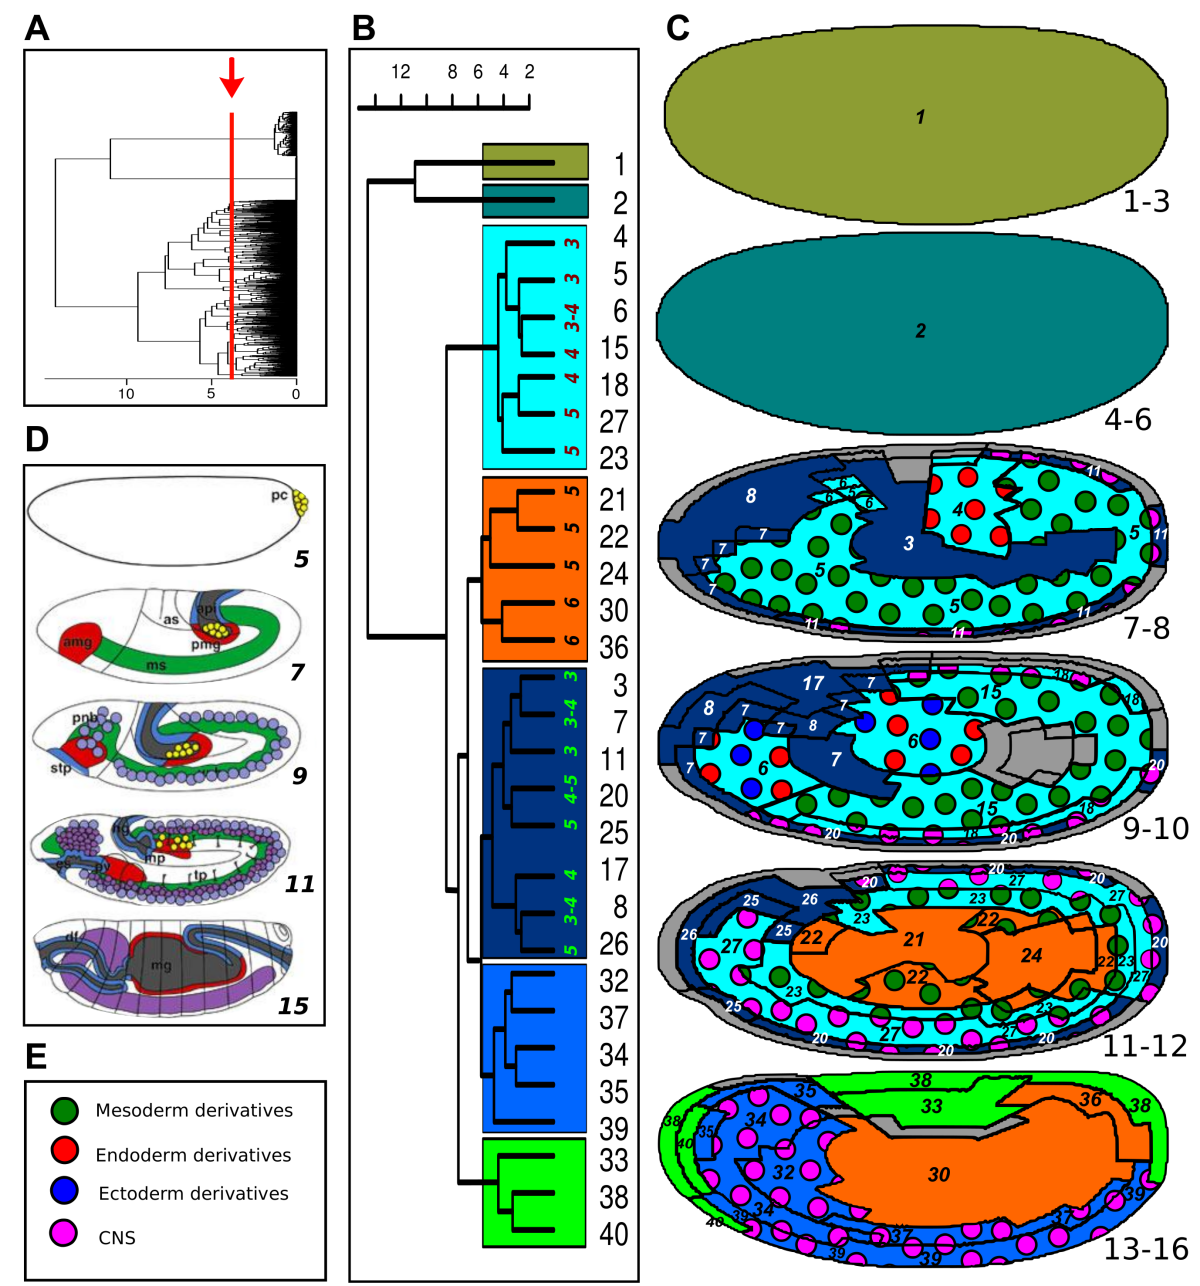
\includegraphics[width=0.65\textwidth]{./Images/Art-I/territories.png}
  \centering
  \caption{Synexpression territories (ST). (A) Dendrogram produced by hierarchical clustering on a similarity matrix (pearson's correlation) of all the embryo regions of the six stages. Red line shows the cut-off to produce 40 STs. (B) Dendrogram reconstructed using only territories with at least 50 genes with a minimum specificity (I, methods). The coloured boxes show the main branches of the dendrogram. The number indicated inside the boxes represent the stages each ST corresponds to (3 is stage 7-8, 4 is stage 9-10, 5 is stage 11-12 and 6 is stage 13-16). The ST number is at the right. (C) STs mapped onto the embryo. Gray regions have less than 50 genes expressed. Background color refers to which `meta-territory' (in B) each ST is part of. Coloured circles represent GOterm enrichment of a specific tissue/germ layer derivative (shown in E). Stages in the lower-left part of each embryo. From stage 7-8, the ST number (as in B) is indicated. (D) Hartenstein's embryo schemes \citep{Hartenstein1993} with their respective stages in the left upper part. (E) Colour code of specific tissue/germ layer derivative used in C.)}
  \label{fig:Art-I-territories}
\end{figure}

In summary, the STs and their spatial distribution largely reconstruct the known compartmentalization of the embryo. First A/P and D/V compartments are formed (stage 3-4), later germ-band, non-germ-band and posterior midgut compartments (stage 7-8), the germ-band then splits into foregut, hindgut and rest of mesoderm while the nervous system starts to differentiate (stage 9-10) and finally the midgut territories arise (stage 11-12).
Therefore, this specific sequence resembles the expected one based on changes in embryonic anatomy and fate maps collected over many years and analysed qualitative (Hartenstein, 1993). 
Thus, my study reinforce this compartmentalization time line using the spatio-temporal expression of hundreds of genes.

%%%%%%%%%%%%%%%%%%%%%%%%%%%%%%%%%%%%%%%%%%%%%%%%%%%%%%%%%%%%%%%%%%%%%%%%%%%%%%%%%%%%% 
%	\clearpage
%\section{Complexity and compartmentalization in \textit{Ciona}}
%	\subsection{Major increase in compartmentalization and disparity after gastrulation}
%objective
With \textit{Ciona}, I measured compartmentalization combining gene expression data at the individual cell-level (until gastrula) or tissue level (tailbud stages) with various 3D embryo models.
Therefore, in here I will refer to relative volume of expression (instead of area as previously)
%results
Globally, the volume of expression decreases mostly after gastrulation (between the 112-cell and the early tailbud stage).
However less dramatic, I found significant differences between the 32-cell and 64-cell stages, and between the 64-cell and 112-cell stages.

As expected, the major increase in disparity happens also occurs between the 112-cell and the early tailbud stage (II, Fig. 4).
I also found a significant increase in disparity in the 64 to 112-cell stages and early to mid-tailbud stages transitions.
Importantly, I found no significant differences between the relative volume of expression of the early and mid-tailbud (II, Fig. 3A), but I found a significant difference between their disparity.

%discussion

This means that, on average, genes are expressed in a similar number of tissues in these stages, but in the mid tailbud the combination of genes expressed in these tissues are more different between each other. This shows that the disparity measure is complementary to the relative volume measure to describe the compartmentalization of the embryo.

In contrast to what I found in \textit{Drosophila}, the major change in compartmentalization in \textit{Ciona} occurs clearly after gastrulation.
In \textit{Ciona}, early embryonic patterning is based on maternal determinants and signalling events mostly between neighbouring cells \citep{Lemaire2009}, which act in a combinatorial way \citep{Hudson2007} to establish a unique TF combination in more than half of the blastomere pairs before gastrulation \citep{Imai2006} determining most of their fates.
Thus, even when in \textit{Ciona} most of the cell fates are already determined (by the specific combination of a fraction of TFs) and the embryo can be said to be already highly compartmentalized, this is not evident at the global level of gene expression, which I am measuring here.
This `delay' could be explained by the relatively slower process of signal transduction (as in \textit{Ciona}) compared to the gap gene network (in \textit{Drosophila}).

%%%%%%%%%%%%%%%%%%%%%%%%%%%%%%%%%%%%%%%%%%%%%%%%%%%%%%%%%%%%%%%%%%%%%%%%%%%%%%%%%%%%% 
\subsection{The leading role of TFs and SIGs}
%objective
I then tested if in \textit{Ciona} the TFs and signalling molecules (SIGs) also showed an early compartmentalization, expected from their allegedly leading role in early pattern formation.
	\nomenclature{SIGs}{Signaling molecules}
	\nomenclature{RTK}{receptor tyrosine kinase}
SIGs consist of genes of receptor tyrosine kinase (RTK) pathways such as FGFs and intracellular signalling molecules such as MAPK, Notch, Wnt, TGF$\beta$, Hedgehog and genes in the JAK/STAT pathways (based on \citealp{Imai2004}) 

%results 1
As expected, TFs volume of expression decreased faster than non-TFs. The TFs showed lower volume of expression in the 64-cell and 112-cell stages (II, Fig. 3B). The results are similar for maternal and zygotic genes (maternal/zygotic classification based on \citealp{Matsuoka2013}; II,Fig. S1).
I then compared TF families (categories based on \citealp{Imai2004}) and found that six TF families showed lower relative volume in the early gastrula (BZIP, T-box, bHLH, HMG, Nuclear Receptor, and `Other-TFs') but only T-box genes showed a lower relative volume from the 32-cell stage until gastrula (II,Fig. S2). 

%discussion 1
The results obtained for the T-box gene family (conserved in metazoan and several non-metazoan lineages \citep{Sebe-Pedros2013}) are consistent with the known important role these genes have in diverse metazoan species early cell fate specification (reviewed in: \citealp{Papaioannou2014,Showell2004}.
Examples of T-box genes in \textit{Ciona} are Tbx6 and \textit{brachyury}, crucial for muscle tissue formation \citep{Mitani1999,Nishida2005} and for notochord specification \citep{Yasuo1998}, respectively.
 
%results 2
SIGs showed significant lower relative volume of expression than the rest of the genes in the 32-cell, 64-cell, and 112-cell stages (II, Fig. 3B).
Specifically, in the 64-cell stage RTK-MAPK, Wnt and TGF$\beta$ families showed significant higher disparity in the 64 cells stage, suggesting a predominant role of these pathways in the patterning of the embryo at this stage. 
%discussion2
This is consistent with known short range induction events by nodal and various FGFs, which are part of the TGF$\beta$ and RTK-MAPK signalling pathways, respectively \citep{Lemaire2008}.
%general discussion? (X)


%%%%%%%%%%%%%%%%%%%%%%%%%%%%%%%%%%%%%%%%%%%%%%%%%%%%%%%%%%%%%%%%%%%%%%%%%%%%%%%%%%%%% 
\subsection{3D roughness increases non-linearly}
%objective
In here I used the Dirichlet Normal Energy (DNE; \citealp{Winchester2016}) as a measure of complexity that considers the overall curvature of the 3D surface of a gene expression pattern.
Importantly, DNE can also be analysed at different spatial scales. 
	\nomenclature{DNE}{Dirichlet Normal Energy}
Therefore, DNE would be the 3D equivalent of the roughness measure I used for \textit{Drosophila}.

%results
DNE values increase throughout development (II, Fig. 5), again with the major change between the 112-cell and the early tailbud. 

The max (mean of the last decile) values increase substantially already between the 64 and 112 cells stages (with 1000 and 10000 polygonal faces), while the min values (mean of the first decile) remain practically constant during development, showing that the most complex patterns in each stage get increase their DNE value but there is always a proportion of very simple expression pattern.
Also, I found that at low spatial scales (1000 and 10000 polygons per mesh; II, Fig. 5) I found that the mean DNE of the late tailbud is higher than at the mid tailbud (one-way ANOVA pvals < 0.05).
	\nomenclature{ANOVA}{Analysis of Variance}

%discussion
In summary, this results show that the complexity of distribution in 3D space of cells/tissues expressing a gene (measured with DNE) increases through development, as even when the increase was more pronounced just after gastrulation, significant changes were found before and after this.

%%%%%%%%%%%%%%%%%%%%%%%%%%%%%%%%%%%%%%%%%%%%%%%%%%%%%%%%%%%%%%%%%%%%%%%%%%%%%%%%%%%%% 
\subsection{Synexpression territories in \textit{Ciona}}
%objective
Because in the tailbud stages the information is based on tissues and not on individual cells as the early stages, I analysed the synexpression territories (STs) of these stages separately by means of a hierarchical clustering (II, Methods). As in Drosophila, how the different STs cluster with each other is informative of the degree of differentiation between stages. If STs cluster with other STs in the same stage, it would mean that the majority of genes change their expression in a similar way over time independently of where they are. If STs cluster with other STs in the same part of the
embryo in successive stages, it would mean that this part of the embryo has expression dynamics independent from other parts of the embryo, which would be expected in already differentiated cells/tissues.

%results
Early stages STs cluster by stage. Thus, even if at the first three stages a high proportion of blastomeres express a nearly unique combination of transcriptional factors \citep{Imai2006}, the bulk change in gene expression is common to all blastomeres. Within each early stage, STs coincides very well with the know fate map (II, Fig 6A; II, Fig. S8), with some exceptions That I describe in the next subsection.

In contrast, in tailbud stages practically all STs cluster by tissue/cell type, which indicates that the in early tailbud, most tissues are already quite differentiated.
This is largely consistent with the bulk of other studies analyzing these stages at the level of individual or small sets of genes \citep{Corbo1997,DiGregorio1999}.

%discussion 2
The early stages analysis is similar to one made by \citet{Imai2006}, who used the expression profile of 53 zygotically TFs in single cells in the 16, 32, 64, and 112-cell stages, to perform a hierarchical clustering (for each stage separately). My analysis is different in two aspects: I performed the clustering using the blastomeres of different stages and my analysis is not restricted to TFs. As I said previously, using various stages is informative of the overall differentiation process and can be used to discern between differentiation scenarios, as the differences between early and tailbud stages I found here.

\begin{figure}[h]
  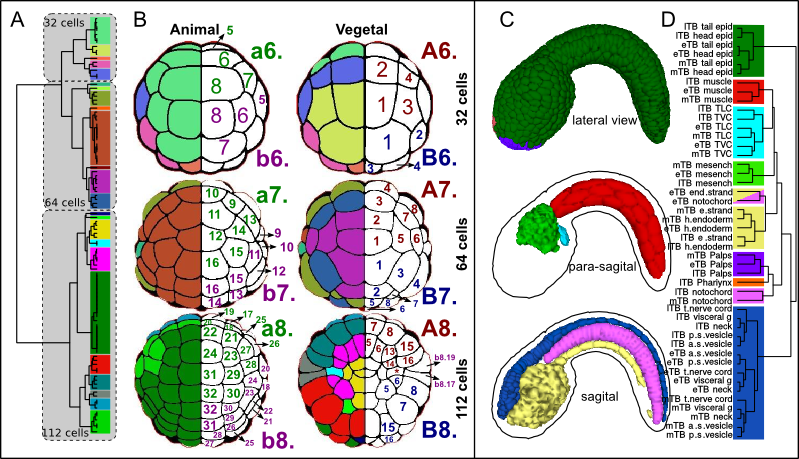
\includegraphics[width=\textwidth]{./Images/Art-II/territories.png}
  \centering
  \caption{Ciona synexpression territories. 
  (A) Dendrogram produced by hierarchical clustering of cells in 32-cell, 64-cell and 112-cell stages. Dashed boxes show that STs cluster by stage. Coloured boxes show the cut-off to produce 24 STs.
  (B) Names of cells (Conklin nomenclature; \citealp{Conklin1905}) indicated with a prefix shown at right. STs in the 32 cells, 64 cells and 112 cells stages (top, middle and bottom, respectively). Colour refers to which ST of the dendrogram (in A) each cell is part of. Animal view based on \citet{Nicol1988} and vegetal view based on \citet{Cole2004a}. The cell marked with a star (*) is the A7.6 cell, that in this analysis represents their descendant cells (A8.11 and A8.12).
  C) Dendrogram produced by hierarchical clustering of tissues in early, mid and late tailbud stages. The coloured boxes show the cutoff to produce 10 STs. (D) STs in the tailbud stages shown in a lateral, para-sagital and sagital views of a mid tailbud 3D embryo model (from \citealp{Nakamura2012}). Colour refers to which ST of the dendrogram (in C) each tissue is part of.
}
  \label{fig:Art-II-territories}
\end{figure}

%%%%%%%%%%%%%%%%%%%%%%%%%%%%%%%%%%%%%%%%%%%%%%%%%%%%%%%%%%%%%%%%%%%%%%%%%%%%%%%%%%%%% 
\subsection{Discrepancies between fate map and STs}

I found a few cases in which cells with the same fate where contained in different STs. This would be the case of: 1) cells whose fate is disproportionally affected or determined by a small number of genes (as this analysis reflect quantitative differences at the level of hundreds of expressed genes
but can not distinguish between the relative importance of each gene) or 2) cells that although having a restricted fate at a certain stage their differentiation is not complete (at the level of gene expression).

An example of the latter is a ST in the 112-cell stage (in magenta; Fig. X) that contains   precursors of the notochord (A8.5, A8.6, A8.13, and A8.14, B8.6) and mesenchyme (B8.5) \citep{Tokuoka2004}.
The latter come from a secondary notochord/mesenchyme bipotential cell (B7.3). It has been reported that the expression of Twist-like 1, necessary for mesenchyme differentiation, starts at this stage \citep{Imai2003}.
This evidence, together with the inclusion of the mesenchyme cell in this otherwise exclusively notochord territory (primary and secondary), seems to indicate that the differentiation of cell pair B8.5 as mesenchyme is still incomplete at this stage.

\subsection{Gene expression dynamics in cell-lineages}

I analysed the gene expression similarity between lineage-related cells (i.e., between daughters cells and between mother/descendants cells) in the early stages (II, Fig. 8).
In general, cells are more closely genetically to their sister cells than to their mother/descendants, which is reflected in the clustering of STs by stages discussed before.
I found also that at the 64-cell stage, cells that show more genes expressed differently than
their ancestors are neural fated cells, which might be related with the fact the unrestricted state of these cells at this stage (i.e., their descendants will give rise to different cell fates).
%	\clearpage

%\section{Compartmentalization and complexity measures}
%	\input{./Parts/Results_Art_.tex}
%	\clearpage

\section{Comparative study between \textit{Drosophila} and \textit{Ciona} (I and II)}
	\subsection{Compartmentalization}
%objective
%I estimated the degree of compartmentalization calculating the relative area or volume of expression of genes during development.
%My intention here was not to focus on individual genes, but to get a global overview of the embryo compartmentalization and differentiation processes based on expression data of thousands of genes, i.e., using a statistical approach.
%
%One would expect, and it has been implicitly assumed \citep{Carroll2001} \citep{Davidson2001} that the compartmentalization of the embryo (as I measure it here) increases during development.
%However, the specific temporal dynamics of this increase in any species is not known. Neither is clear if the dynamics should be similar for different species, or for different groups of genes.

As the development of \textit{Ciona} and \textit{Drosophila} are very different and it would be impossible to compare them stage-by-stage, I focused here in three major developmental periods: pre-gastrula, gastrula, and post-gastrula stages. These periods are easily recognizable in both species facilitating the comparative analysis.

%results
I found that in both species, the relative area or volume decreased in a non-linear way (see Fig. \ref{fig:Art-I-3measures} and Fig. \ref{fig:Art-II-3measures}). 
However, the timing of the major decrease was different.
In \textit{Drosophila} the major decrease occurred at very early development, from maternal to early gastrula stage (Fig. \ref{fig:Art-I-3measures}).
Practically half of the genes in follows this decrease pattern: 46\% of the genes were characterized as having a non-linear decrease in their relative area.
In contrast, in \textit{Ciona} the volume of expression decreases mostly after gastrulation (between the 112-cell and the early tailbud stage).
However less dramatic, I found significant differences between the 32-cell and 64-cell stages, and between the 64-cell and 112-cell stages.

%%%%%%%%%%%%%%%%%%%%%%%%%%%%%%%%%%%%%%%%%%%%%%%%%%%%%%%%%%%%%%%%%%%%%%%%%%%%%%%%%%%%%%%%%%%%%%%%%%%%%%%%%%%%%%
\begin{figure}[b]
  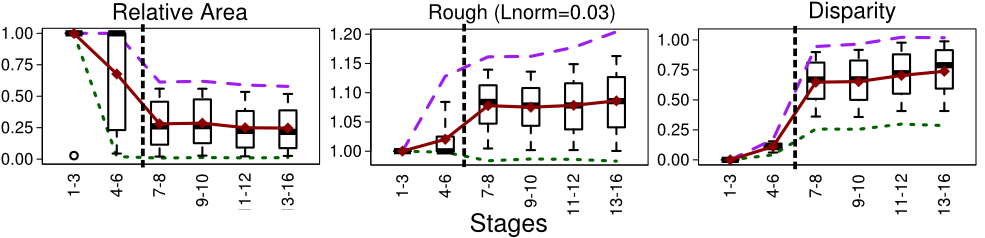
\includegraphics[width=\textwidth]{./Images/Art-I/3_measures.png}
  \centering
  \caption{\textbf{Measures in \textit{Drosophila}}.Distribution plot of the relative area of expression (left), roughness (center) and disparity (right) for all genes in each stage. Diamonds represent the mean, boxes the Inter Quartile Range (IQR). Whiskers 10 and 90 percentiles. Dashed line represents the max values and dotted line the min values (mean of the last and first decile, respectively). Stages on the x-axis, vertical dashed line represents gastrulation entry.
	\nomenclature{IQR}{Inter Quartile Range} 
  }
  \label{fig:Art-I-3measures}
\end{figure}
%%%%%%%%%%%%%%%%%%%%%%%%%%%%%%%%%%%%%%%%%%%%%%%%%%%%%%%%%%%%%%%%%%%%%%%%%%%%%%%%%%%%%%%%%%%%%%%%%%%%%%%%%%%%%%


% discussion
The difference in the timing of the major change on compartmentalization between species must relate to differences in their specific development.
The earlier compartmentalization of \textit{Drosophila} is most probably due to its derived early development, namely, the syncytial blastoderm. 
During the blastoderm stage, approximately 4,000 cell nuclei can `communicate' with each other only by TFs \citep{Jaeger2011}. The direct cross regulation of gene expression facilitates a rapid and highly dynamic process which seems to be responsible for the early spatial restriction of a great proportion of developmental genes.
It could be therefore expected that these early increase in complexity in \textit{Drosophila} would be shared by all insects with a syncitial blastoderm stage. Also, it could be that the early increase in complexity might be affected by the number of cell divisions that occur until the blastoderm is cellularized. It is known that \textit{Drosophila} cellularizes relatively late (so there is more time for patterning within the syncitial bastoderm). In contrast, the desert locust (\textit{Schistocerca gregaria}) cellularization occurs very early, even before the formation of the blastoderm \citep{Ho1997}.

In contrast,  \textit{Ciona}'s early embryonic patterning is based on maternal determinants and signalling events mostly between neighbouring cells \citep{Lemaire2009}, which act in a combinatorial way \citep{Hudson2007} to establish a unique TF combination in more than half of the blastomere pairs before gastrulation \citep{Imai2006} determining most of their fates.
Thus, even when in \textit{Ciona} most of the cell fates are already determined (by the specific combination of a fraction of TFs) and the embryo can be said to be already highly compartmentalized, this is not evident at the global level of gene expression, which I am measuring here.


Therefore, the "delay" of compartmentalization observed in \textit{Ciona} could be explained by the relatively slower process of signal transduction (as in \textit{Ciona}) compared to the gap gene network (in \textit{Drosophila}).

%One would expect, and it has been implicitly assumed \citep{Carroll2001} \citep{Davidson2001} that the compartmentalization of the embryo (as I measure it here) increases during development. However, the specific temporal dynamics of this increase in any species has not been measured until now.


%%%%%%%%%%%%%%%%%%%%%%%%%%%%%%%%%%%%%%%%%%%%%%%%%%%%%%%%%%%%%%%%%%%%%%%%%%%%%%%%%%%%%
\subsection{Disparity}
%objective
As the relative area (or volume) of expression informs on how genes are expressed in progressively smaller regions in the embryo, the disparity measure can inform about how different regions of the embryo express increasingly different combinations of genes.
%Therefore, both measures reflect slightly different aspects of complexity that are independent from each other. A decrease in the volume of expression of genes does not necessarily imply an increase in spatial disparity: genes could decrease their volume of expression but end up restricted to the same parts of the embryo. 
%If the majority of genes would be expressed ubiquitously (this is large volume), however, then the mean disparity between its regions would be necessarily low. 
%
%results
My results show that in each species, the global disparity pattern is similar to the relative area or volume patterns.
Therefore, in \textit{Drosophila} the disparity increases mostly in the transition from the maternal to early gastrula and in Ciona this major change occurs after gastrulation.

%%%%%%%%%%%%%%%%%%%%%%%%%%%%%%%%%%%%%%%%%%%%%%%%%%%%%%%%%%%%%%%%%%%%%%%%%%%%%%%%%%%%%%%%%%%%%%%%%%%%%%%%%%%%%%
\begin{figure}[b]
  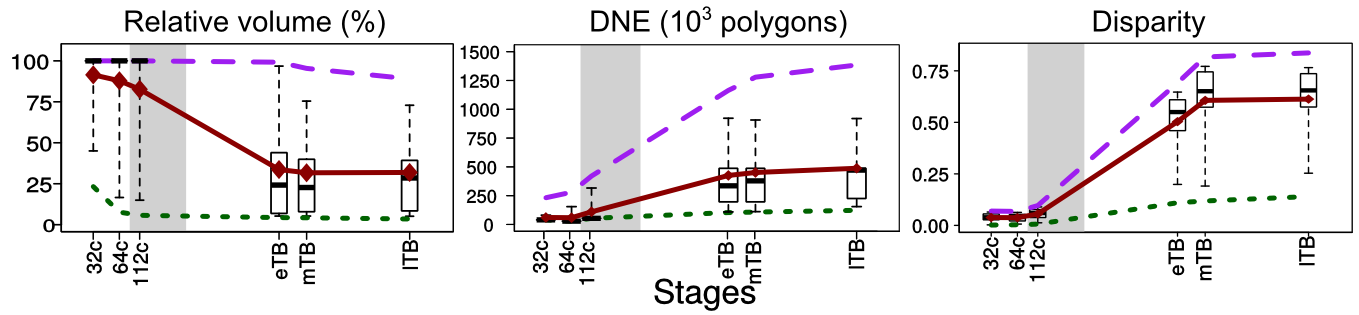
\includegraphics[width=\textwidth]{./Images/Art-II/3_measures_nostars.png}
  \centering
  \caption{\textbf{Measures in \textit{Ciona}.} Distribution plot of the relative volume of expression (left), DNE (center) and disparity (right) for all genes in each stage. Diamonds represent the mean, boxes the IQR. Whiskers 10 and 90 percentiles. Dashed line represents the max values and dotted line the min values (mean of the last and first decile, respectively). Stages on the X-axis (s32c, 32-cells; s64c, 64-cells; s112c, 112-cells; eTB, early tailbud; mTB, mid tailbud; lTB, late tailbud). Grey area represents gastrulation period.}
  \label{fig:Art-II-3measures}
\end{figure}
%%%%%%%%%%%%%%%%%%%%%%%%%%%%%%%%%%%%%%%%%%%%%%%%%%%%%%%%%%%%%%%%%%%%%%%%%%%%%%%%%%%%%%%%%%%%%%%%%%%%%%%%%%%%%%

% discussion
It is important to notice that these measures should not necessarily correlate (see section \ref{measures_relations}.
%
In \textit{Ciona} I found an example of a case when there is no perfect correspondence between the relative volume and the disparity of expression: disparity increased significantly between early to mid-tailbud stages but no significant differences between the relative volume of expression of these stages were found (II, Fig. 3A).
This means that, on average, genes are expressed in a similar number of tissues in these stages, but in the mid tailbud the combination of genes expressed in these tissues are more different between each other.

This shows that the disparity measure is useful specially when is complemented with the relative area (or volume) measure to describe the compartmentalization of the embryo.

%%%%%%%%%%%%%%%%%%%%%%%%%%%%%%%%%%%%%%%%%%%%%%%%%%%%%%%%%%%%%%%%%%%%%%%%%%%%%%%%%%%%% 

\subsection{The leading role of TFs and GFs (and other signalling molecules)}

%%%%%%%%%% articulo 1
%objective
%I wanted the test in both species if TFs and GFs showed an earlier compartmentalization or greater disparity when compared to the rest of the genes. This would be expected from their allegedly leading role in early pattern formation.

%results 1
Using a GOterm analysis in \textit{Drosophila}, I found that TFs (GO:0003700) and GFs (GO:0008083) showed smaller relative area of expression that the rest of genes in the blastoderm stage (Fig. \ref{fig:Art-I-3measures}).
	\nomenclature{GF}{Growth Factor}
	\nomenclature{KW}{Kruskal-Wallis test}
%
The TFs are also expressed in smaller areas than the rest of the genes in all subsequent stages, while the GFs are expressed in smaller areas at the blastoderm (stage 4-6) and extended germ band stages (stage 9-10 and 11-12) (I, Fig.4). In the blastoderm stage the disparity of the regions based only on the TFs is much greater than the one based on all the genes ((KW pvalue $<0.001$, see study I) confirming that these genes account for a large portion of the diversity of gene expression patterns in the blastoderm stage.

%discussion 1
These results are consistent with a previous study of TFs expression during \textit{Drosophila} embryogenesis done by \citet{Hammonds2013}.
They made an extensive analysis of TFs expression using manual annotation of gene expression based on an anatomical controlled vocabulary and classifying every gene as ubiquitous, patterned, ubiquitous-patterned, or maternal (from the BDGP database; \citealp{Tomancak2007}).
They found that the fraction of TFs expressed in a restricted pattern (assigned to a tissue) was higher, when compared to other genes, in all zygotic stages with the exception of the stage 13-16. 
The results I show for stages 4-6, 7-8, 9-10 and 11-12 are consistent with Hammonds et al., as the higher proportion of the TF genes showing a restricted or tissue-specific expression pattern would imply that TFs are expressed in smaller areas in the embryo. For the 13-16 stage, contrary to these authors, I showed that the TFs are highly compartmentalized. This might indicate a limitation of the annotation method used by Hammonds et al., to capture the high spatial compartmentalization of the TFs in this stage.

%%results & discusion 2
%

%%%%%%%%%%%%%%%% articulo 2 
%objective
In \textit{Ciona}, I performed a similar analysis using the categorization of TFs and signaling molecules (SIGs) made by \citet{Imai2004}.
SIGs consist of genes of receptor tyrosine kinase (RTK) pathways such as FGFs and intracellular signalling molecules such as MAPK, Notch, Wnt, TGF$\beta$, Hedgehog and genes in the JAK/STAT pathways \citep{Imai2004}. 

	\nomenclature{SIGs}{Signaling molecules}
	\nomenclature{RTK}{receptor tyrosine kinase}

%results 1
As expected, TFs volume of expression decreased faster than non-TFs. The TFs showed lower volume of expression in the 64-cell and 112-cell stages (II, Fig. 3B). 
The results are similar for maternal and zygotic genes (maternal/zygotic classification based on \citealp{Matsuoka2013}; II,Fig. S1). I then compared TF families and found that six TF families showed lower relative volume in the early gastrula (BZIP, T-box, bHLH, HMG, Nuclear Receptor, and `Other-TFs') but only T-box genes showed a lower relative volume from the 32-cell stage until gastrula (II,Fig. S2). 

%discussion 1
The results obtained for the T-box gene family (conserved in metazoan and several non-metazoan lineages \citep{Sebe-Pedros2013}) are consistent with the known important role these genes have in diverse metazoan species early cell fate specification (reviewed in: \citealp{Papaioannou2014,Showell2004}.
Examples of T-box genes in \textit{Ciona} are Tbx6 and \textit{brachyury}, crucial for muscle tissue formation \citep{Mitani1999,Nishida2005} and for notochord specification \citep{Yasuo1998}, respectively.
%results 2
I also found that the SIGs showed significant lower relative volume of expression than the rest of the genes in the 32-cell, 64-cell, and 112-cell stages (II, Fig. 3B).
Specifically, in the 64-cell stage RTK-MAPK, Wnt and TGF$\beta$ families showed significant higher disparity in the 64 cells stage, suggesting a predominant role of these pathways in the patterning of the embryo at this stage. 
%discussion2
This is consistent with known short range induction events by nodal and various FGFs, which are part of the TGF$\beta$ and RTK-MAPK signalling pathways, respectively \citep{Lemaire2008}.

%general discussion? (X)

In general, the fact that in these two species that display a very different development TFs and GFs (or SIGs in the case of \textit{Ciona}) are more compartmentalized than the rest of the genes precisely in the stage before entering gastrulation, is consistent with these genes having a special role in pattern formation and compartmentalization.
Therefore, my results support the hypothesis of the leading role of TFs and GFs in driving pattern formation and compartmentalization in the early embryo.

%%%%%%%%%%%%%%%%%%%%%%%%%%%%%%%%%%%%%%%%%%%%%%%%%%%%%%%%%%%%%%%%%%%%%%%%%%%%%%%%%%%%% 
%%%%%%%%%%%%%%%%%%%%%%%%%%%%%%%%%%%%%%%%%%%%%%%%%%%%%%%%%%%%%%%%%%%%%%%%%%%%%%%%%%%%% 
\subsection{2D and 3D roughness analyses}
%% objective
%
%I wanted to test the hypothesis of gene expression spatial patterns becoming more complex during development.
%In here, with gene expression spatial pattern I mean the spatial distribution of the cells or tissues expressing a specific gene. 
%
%Considering that I had information in 2D in \textit{Drosophila} and in 3D in \textit{Ciona}, it was necessary to apply a specific method for each species.
As explained in the methods, in order to test the hypothesis of gene expression spatial patterns becoming more complex during development, I developed a I developed a `roughness' measure \citep{Salvador-Martinez2015} for \textit{Drosophila}, which accounts for the curvature of the contour in a 2D gene expression pattern, normalizing it with the contour of a circle of the same perimeter.
In \textit{Ciona}, I applied a similar measure of curvature in 3D, called `Dirichlet normal energy' (DNE), which quantifies the deviation of a surface from being planar \citep{Bunn2011}. To improve the readability of the text,  I will refer to the roughness measure in \textit{Drosophila} as 2D roughness and to the DNE measured used in \textit{Ciona} as 3D roughness.
	\nomenclature{DNE}{Dirichlet Normal Energy}
Both measures not only inform about the overall imbrication or convolution of the shape of a gene expression pattern, but also do it at different spatial scales.
%
%In the following paragraphs, to improve the readability of the text,  I will refer to the roughness measure implemented in \textit{Drosophila} as 2D roughness and to the DNE measured used in \textit{Ciona} as 3D roughness.
%

%results
The results show that both 2D and 3D roughness increase in a non-linear way during development.
As with the compartmentalization and disparity, the difference between species is where the major change is found. 

%drosophila
In \textit{Drosophila}, the major change is found in the transition from the blastoderm to the early gastrula (Fig. \ref{fig:Art-I-3measures}).
When analysing the maximal values (mean of the last decile) it can be seen that they increase initially in the pre-gastrula, reach a stationary phase at mid-embryogenesis and finally increase in the last stages. 
The maximal values are informative about the overall morphological spatial complexity of the embryo in a given stage.
When comparing roughness at different spatial scales (I, Methods), I found that in the last three stages the roughness values are significantly higher at smaller spatial scales is significantly higher that at the higher spatial scales.(Fig. S2 in article I). 

%Ciona
In Ciona, the 3D roughness increase throughout development (II, Fig. 5), with the major change between the 112-cell and the early tailbud (Fig. \ref{fig:Art-II-3measures})  
The max (mean of the last decile) values increase substantially already between the 64 and 112 cells stages (with 1000 and 10000 polygonal faces), while the min values (mean of the first decile) remain practically constant during development, showing that the most complex patterns in each stage get increase their DNE value but there is always a proportion of very simple expression pattern.
Also, I found that at low spatial scales (1000 and 10000 polygons per mesh; II, Fig. 5) I found that the mean DNE of the late tailbud is higher than at the mid tailbud (one-way ANOVA pvals < 0.05).
	\nomenclature{ANOVA}{Analysis of Variance}

%% general discussion
In summary, this results show that the complexity of distribution in space of cells/tissues expressing a gene increases through development, and that these complexity (measured with the 2D and 3D roughness) increase in both \textit{Ciona} and \textit{Drosophila} in a similar way than the other two measures, compartmentalization and disparity.
Also, by analysing the roughness at different scales, I found compelling evidence that complexity may be increasing not only through all the development but also that it does at finer spatial scales over time.

%%%%%%%%%%%%%%%%%%%%%%%%%%%%%%%%%%%%%%%%%%%%%%%%%%%%%%%%%%%%%%%%%%%%%%%%%%%%%%%%%%%%% 
\subsection{Synexpression territories}
%objective
%I wanted to explore in both species the relative degree of similarities between different parts of the embryo within and between different developmental stages.
%
%To do this I used two different approaches, based on the differences between the databases I used for each species.
%In \textit{Drosophila} I used the polar regions with which I computationally divided the embryo. In \textit{Ciona}, I took advantage of the available information at the individual cell/tissue.  

In both species I used a clustering algorithm to produce dendrogram representing the relative degrees of similarities between all regions of different stages at the same time (Fig. \ref{fig:Art-I-territories} and Fig. \ref{fig:Art-II-territories}).
I will refer to the regions that clustered together as "synexpression territories" (STs).
	\nomenclature{ST}{Synexpression territories}

%%%%%%%%%% drosophila
In \textit{Drosophila}, after cutting the dendrogram at a specific threshold and filtering out STs with less than 50 genes expressed with a minimum specificity (see methods in I for a detailed description), 30 STs were selected for further analyses (Fig. \ref{fig:Art-I-territories} B).

%Finally, I grouped the STs in eight `meta-territories' to analyse how the different STs relate between them.
Finally, I grouped the STs in eight `meta-territories', as I wanted not only to see how the regions in the embryo formed different STs, but also how different STs cluster with each other, as this is informative of the degree of differentiation between stages. If STs cluster with other STs in the same stage, it would mean that the majority of genes change their expression in a similar way over time independently of where they are.
If STs cluster with other STs in the same part of the embryo in successive stages, it would mean that this part of the embryo has expression dynamics independent from other parts of the embryo, which would be expected in already differentiated cells/tissues.

%%%%%%%%%%%%%%%%%%%%%%%%%%%%%%%%%%%%%%%%%%%%%%%%%%%%%%%%%%%%%%%%%%%%%%%%%%%%%%%%%%%%%%%%%%%%%%%%%%%%%%%%%%%%%%
\begin{figure}[ht]
  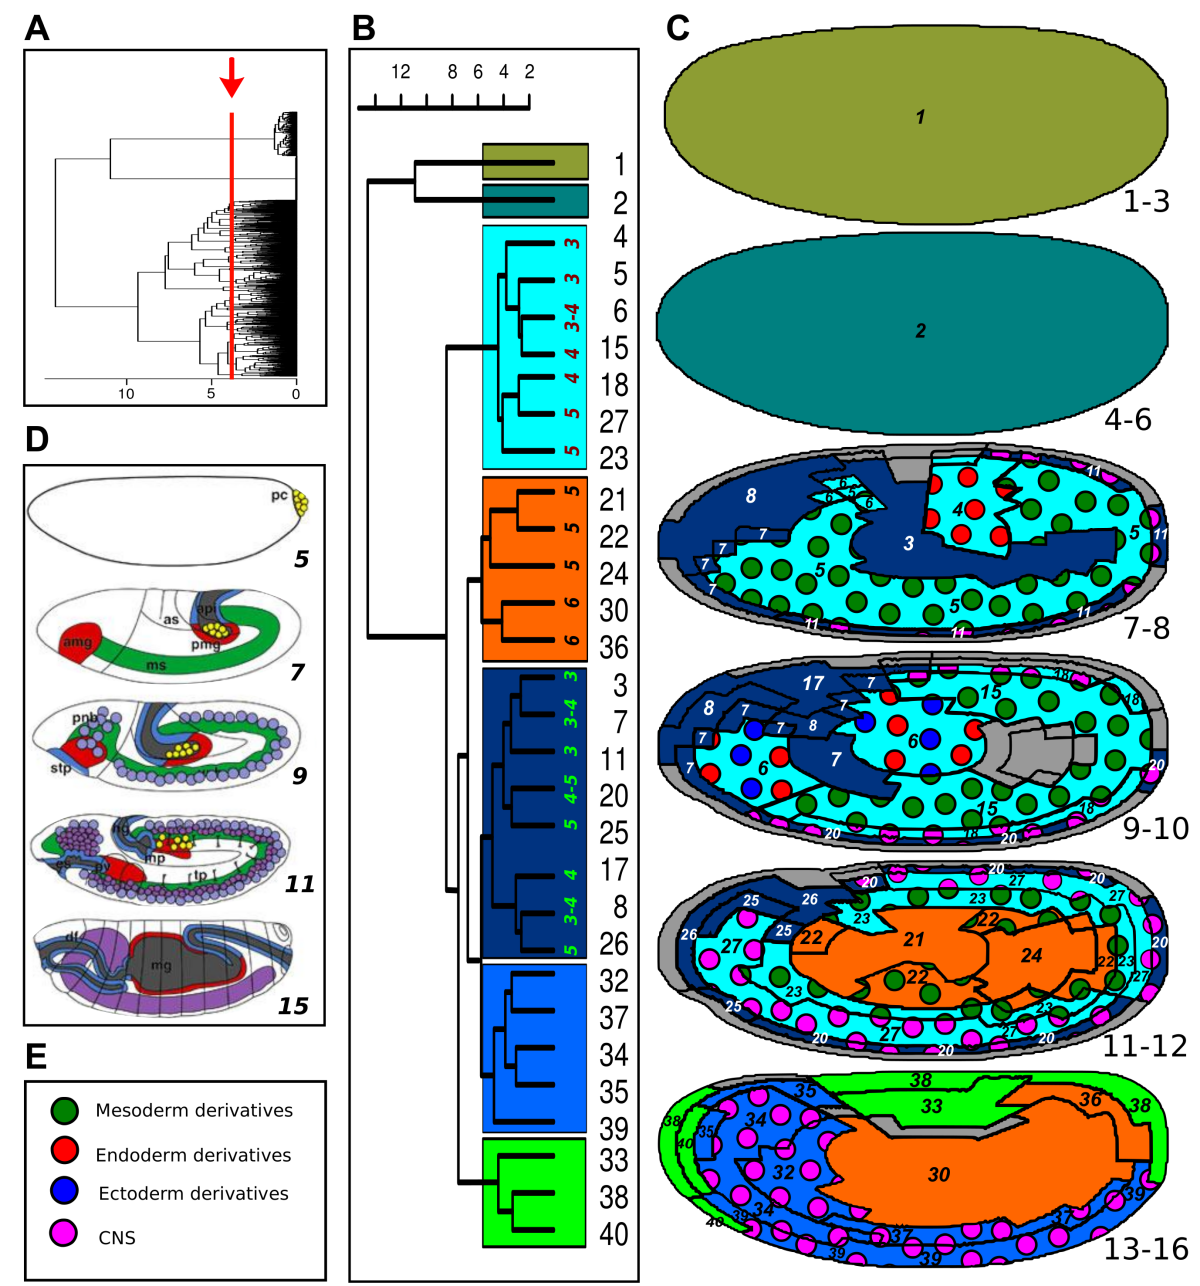
\includegraphics[width=0.65\textwidth]{./Images/Art-I/territories.png}
  \centering
  \caption{Synexpression territories (ST). (A) Dendrogram produced by hierarchical clustering on a similarity matrix (pearson's correlation) of all the embryo regions of the six stages. Red line shows the cut-off to produce 40 STs. (B) Dendrogram reconstructed using only territories with at least 50 genes with a minimum specificity (I, methods). The coloured boxes show the main branches of the dendrogram. The number indicated inside the boxes represent the stages each ST corresponds to (3 is stage 7-8, 4 is stage 9-10, 5 is stage 11-12 and 6 is stage 13-16). The ST number is at the right. (C) STs mapped onto the embryo. Gray regions have less than 50 genes expressed. Background color refers to which `meta-territory' (in B) each ST is part of. Coloured circles represent GOterm enrichment of a specific tissue/germ layer derivative (shown in E). Stages in the lower-left part of each embryo. From stage 7-8, the ST number (as in B) is indicated. (D) Hartenstein's embryo schemes \citep{Hartenstein1993} with their respective stages in the left upper part. (E) Colour code of specific tissue/germ layer derivative used in C.)}
  \label{fig:Art-I-territories}
\end{figure}
%%%%%%%%%%%%%%%%%%%%%%%%%%%%%%%%%%%%%%%%%%%%%%%%%%%%%%%%%%%%%%%%%%%%%%%%%%%%%%%%%%%%%%%%%%%%%%%%%%%%%%%%%%%%%%

%results
The results show that stages 1-3 and 4-6 each one form a ST. If a cut-off is selected so that stage 4-6 is divided in four sub-territories (I,Fig. S3) the embryo splits in four parts: anterior, posterior, dorsal and ventral.
This correspond to a nearly Cartesian system one could expect from the two signalling systems known in the earliest patterning in \textit{Drosophila} (the A/V and D/V signalling cascades; \citep{Gilbert2014}).
%
The STs seem to coincide with the known embryo fate map (see Fig. \ref{fig:Art-I-territories} D; \citealp{Hartenstein1993}) and many of them are enriched with GOterms that coincide with their expected fate.
For example, in stage 7-8 (just after gastrulation) there is a ST that corresponds spatially with the germband and is enriched with mesodermal GOterms (Fig. Fig. \ref{fig:Art-I-territories} C).

Two meta-territories appear in the last stage (light blue and green, Fig. \ref{fig:Art-I-territories} C), which suggests that the tissues/organs related to those STs differentiate quite late.
%
%% discussion
One of these meta-territories is enriched with terms related to epidermis such as cuticle development ("chitin catabolic process" [GO:0006032] and "cuticle development" [GO:0042335] STs 33 and 38), which coincides with cuticle deposition by epithelial cells during stage 16 \citep{Ostrowski2002}.
%
The other meta-territory corresponds spatially with the CNS of the embryo and is indeed enriched with CNS GO-terms.
The CNS territory is enriched with GOterms like "dendrite morphogenesis" (GO:0048813) and "axon guidance" (GO:0007411). 
	\nomenclature{CNS}{Central Nervous System}

%%%%%%%%%%%%%%%%%%%%%%%%%%%%%%%%%%%%%%%%%%%%%%%%%%%%%%%%%%%%%%%%%%%%%%%%%%%%%%%%%%%%%%%%%
\begin{figure}[ht]
  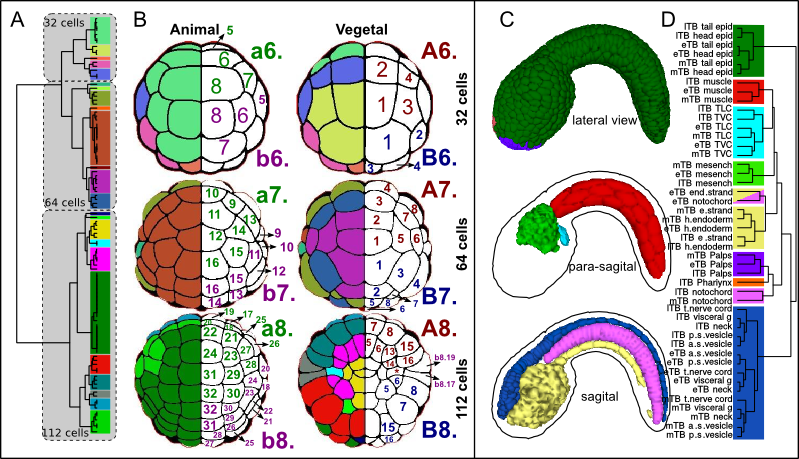
\includegraphics[width=\textwidth]{./Images/Art-II/territories.png}
  \centering
  \caption{Ciona synexpression territories. 
  (A) Dendrogram produced by hierarchical clustering of cells in 32-cell, 64-cell and 112-cell stages. Dashed boxes show that STs cluster by stage. Coloured boxes show the cut-off to produce 24 STs.
  (B) Names of cells (Conklin nomenclature; \citealp{Conklin1905}) indicated with a prefix shown at right. STs in the 32 cells, 64 cells and 112 cells stages (top, middle and bottom, respectively). Colour refers to which ST of the dendrogram (in A) each cell is part of. Animal view based on \citet{Nicol1988} and vegetal view based on \citet{Cole2004a}. The cell marked with a star (*) is the A7.6 cell, that in this analysis represents their descendant cells (A8.11 and A8.12).
  C) Dendrogram produced by hierarchical clustering of tissues in early, mid and late tailbud stages. The coloured boxes show the cutoff to produce 10 STs. (D) STs in the tailbud stages shown in a lateral, para-sagital and sagital views of a mid tailbud 3D embryo model (from \citealp{Nakamura2012}). Colour refers to which ST of the dendrogram (in C) each tissue is part of.
}
  \label{fig:Art-II-territories}
\end{figure}
%%%%%%%%%%%%%%%%%%%%%%%%%%%%%%%%%%%%%%%%%%%%%%%%%%%%%%%%%%%%%%%%%%%%%%%%%%%%%%%%%%%%%%%%%%%%

In \textit{Ciona}, because gene expression information in tailbud stages is based on tissues and not on individual cells as the early stages, I analysed the STs of these stages separately (II, Methods). 

%results
If in the early stages, three "meta-territories" are formed, each one would correspond to one stage, i.e., STs in early stages cluster by stage.
Thus, even if at the first three stages a high proportion of blastomeres express a nearly unique combination of transcriptional factors \citep{Imai2006}, the bulk change in gene expression is common to all blastomeres. Within each early stage, STs coincides very well with the know fate map (II, Fig 6A; II, Fig. S8), with some exceptions I will describe in the next subsection.
%
In contrast, in tailbud stages practically all STs cluster by tissue/cell type, which indicates that the in early tailbud, most tissues are already quite differentiated.
This is consistent with studies analysing these stages at the level of individual or small sets of genes \citep{Corbo1997,DiGregorio1999}.

%discussion 2
This analysis in the early stages is similar to the one made by \citet{Imai2006}, who used the expression profile of 53 zygotically TFs in single cells in the 16, 32, 64, and 112-cell stages, to perform a hierarchical clustering (for each stage separately). 
It is different in two aspects: I performed the clustering using the blastomeres of different stages and my analysis is not restricted to TFs. As I said previously, using various stages is informative of the overall differentiation process and can be used to discern between differentiation scenarios, as the differences between early and tailbud stages I found here.

%%% general discussion

The main difference between species is that, in \textit{Drosophila} the differentiation process continues throughout whole embryogenesis (as new STs were formed until the last stage I analysed) and different organs differentiate at different developmental times.
In contrast, the \textit{Ciona} embryo seems to be already genetically differentiated at the early tailbud (as the STs of all the tissues in the tailbud stages cluster together) so the last embryo stages consist only of moderate morphogenetic movements (mainly cell elongation; \citealp{Hotta2007}).
Therefore, the ST analysis is a valuable tool, based on differential gene expression, to get a global perspective on the local differentiation of the embryo.
%	\clearpage

\section{Main spatio-temporal profiles of gene expression in \textit{Drosophila} (I)}
	%objective
With a time series cluster analysis \citep{Ernst2006} of the relative area of expression, I found the eight main spatio-temporal profiles of gene expression in the embryonic development of \textit{Drosophila} (I, Fig. 5).
%results
As expected, the most common profile (n=297 genes) follows the global profile of non-linear decrease in the first stages (I, Fig 5).

Among the rest of profiles, I found both linear increase and decrease profiles and a `hill-like' profile (initial increase and further decrease with the higher values at stage 7-8)
%
The linear decrease profile (n=167 genes) was enriched with `mitotic cell cycle' (GO:0000278), `RNA processing' (GO:0006396) and `chromatin modification' (GO:0016568) GOterm genes, highlighting biological processes that first are present in the whole embryo and become more and more restricted in space as development proceeds.
%discussion
The `mitotic cell cycle' term, for example, most likely relates to the fast mitotic cycles in the earliest embryo. During stage 1-3 nine fast and synchronic mitotic divisions take place in the entire embryo, then in stage 4-6 mitotic divisions 10-13 occur more slowly, almost synchronically. The 14th cycle, zygotically controlled, is long and of different durations in the embryo.

With a temporal co-expression cluster analysis using microarray data through the life cycle of \textit{D. melanogaster}, \citet{Arbeitman2002} found that most cell cycle genes were expressed at high levels during the first 12h, but only a few are expressed at high level thereafter.
My analysis is consistent with this, as I found that the profile of linear decrease (I, Fig. 5A) is enriched with such genes. In this sense, this study is complementary to Arbeitman et al., and adds the spatial dimension to their temporal expression profiles.

%	\clearpage

\section{Discrepancies between fate map and STs (II)}
	

I found a few cases in \textit{Ciona} in which cells with the same fate where contained in different STs. This would be the case of: 1) cells whose fate is disproportionally affected or determined by a small number of genes (as this analysis reflect quantitative differences at the level of hundreds of expressed genes but can not distinguish between the relative importance of each gene) or 2) cells that although having a restricted fate at a certain stage their differentiation is not complete (at the level of gene expression).

This analysis could not be made in \textit{Drosophila} as the gene expression data is not a the single level resolution.

An example of the latter is a ST in the 112-cell stage (in magenta; \ref{fig:Art-II-territories} B; II, Fig. S8) that contains precursors of the notochord (A8.5, A8.6, A8.13, and A8.14, B8.6) and mesenchyme (B8.5) \citep{Tokuoka2004}.
The latter come from a secondary notochord/mesenchyme bipotential cell (B7.3). It has been reported that the expression of Twist-like 1, necessary for mesenchyme differentiation, starts at this stage \citep{Imai2003}.
This evidence, together with the inclusion of the mesenchyme cell in this otherwise exclusively notochord territory (primary and secondary), seems to indicate that the differentiation of cell pair B8.5 as mesenchyme is still incomplete at this stage.

\subsubsection{Gene expression dynamics in cell-lineages}

I analysed the gene expression similarity between lineage-related cells (i.e., between daughters cells and between mother/descendants cells) in the early stages (II, Fig. 8).
In general, cells are more closely genetically to their sister cells than to their mother/descendants, which is reflected in the clustering of STs by stages discussed before.
I found also that at the 64-cell stage, cells that show more genes expressed differently than
their ancestors are neural fated cells, which might be related with the fact the unrestricted state of these cells at this stage (i.e., their descendants will give rise to different cell fates).
%	\clearpage

\section{Adaptation in \textit{Drosophila} embryogenesis (III and IV)}
	%% objective

I combined the Synexpression Territories (STs) approach with genome-wide coding-region polymorphism data (from the DGRP database) and the coding-region divergence between \textit{D. yakuba} and \textit{D. melanogaster} in order to estimate the  proportion of adaptive non-synonymous substitutions ($\omega_{\alpha}$) in the genes expressed in each ST (n=589 genes; III, Methods).
	\nomenclature{$\omega_{\alpha}$}{Proportion of adaptive non-synonymous substitutions}
	\nomenclature{$\omega$}{dN/dS ratio}
	

Using this approach, I could chart a spatial map of natural selection acting on \textit{Drosophila}'s embryo anatomy.
I complemented this with a analysis using available annotation of gene expression (n=2,835 genes) using a controlled vocabulary of anatomical structures from the BDGP database \citep{Tomancak2007}.

%% results %%%%%%%%%%%%%%%%%%%%%%%%%%%%%%%%%%
The results showed a few STs with significant higher or lower $\omega_{\alpha}$ (permutation test; III, Methods)

%% high OmegaA
\subsection{STs or anatomical terms with high $\omega_{\alpha}$}
STs 13 and 32 (ST number comes from the hierarchical clustering algorithm), which showed a higher $\omega_{\alpha}$, seem to correspond to the forming foregut and hindgut (stage 11-12) and to the CNS (stage 13-16) respectively.
To explore if ST 32 high $\omega_{\alpha}$ was indeed related to the CNS, I separated the genes CNS or not-CNS related.
I found that both groups showed a high $\omega_{\alpha}$, which suggests that in addition to the CNS, another structure in the anterior region would be under positive selection.
 Using the anatomical terms approach, no anatomical terms related to the CNS were found to have high $\omega_{\alpha}$ with the initial criteria.
I therefore applied a more stringent criterion to consider genes as part of an anatomical term (before a gene could have a maximum of seven anatomical terms associated instead of a more stringent number of three) and found that `Embryonic brain' showed high $\omega_{\alpha}$ (permutation test, p = 0.046).
Also, with the anatomical terms approach, I found that genes associated with `Gonads', in the last stage, clearly showed evidence of adaptive evolution (III, Figure 2), which is consistent with previously reported high rates of adaptive substitution in the testes \citep{Akashi1994,Civetta1995,Nuzhdin2004,Proschel2006}

Finally, ST 24 (stage 11-12) that seems to corresponds to part of the trunk mesoderm marginally significant high $\omega_{\alpha}$ (p = 0.061). A similar result was obtained with for the anatomical term `Trunk mesoderm' in stage 9-10 (p =
0.087).

%% low omegaA
\subsection{STs or anatomical terms with low $\omega_{\alpha}$}
STs 20 and 29 with showed low $\omega_{\alpha}$, seem to correspond to the forming midgut (stage 11-12) and to the forming larval digestive system (stage 13-16) respectively.
Similar results are found when using the anatomical term approach, as low $\omega_{\alpha}$ was found in many anatomical terms related to the digestive system in the last stage: `Embryonic midgut', `Embryonic salivary gland', `Embryonic hindgut', `Embryonic proventriculus'. 
Also, combining three related anatomical terms, `Embryonic foregut', `Embryonic epipharynx' and `Embryonic hypopharynx', that separately did not have enough genes to be considered in the analysis, showed low $\omega_{\alpha}$. 

The lack of adaptive change in the forming digestive system might reflect their relative enrichment in metabolic genes \citep{Marianes2013}. The coding regions of metabolic genes have been found to be more conserved than non-metabolic genes \citep{Peregrin-Alvarez2009}.

%%%%%%%%%%%%%%%%%%%%%%%%%%%%%%%%%%%%%%%%%%%%%%%%%%%%%%%%
\begin{figure}[h]
  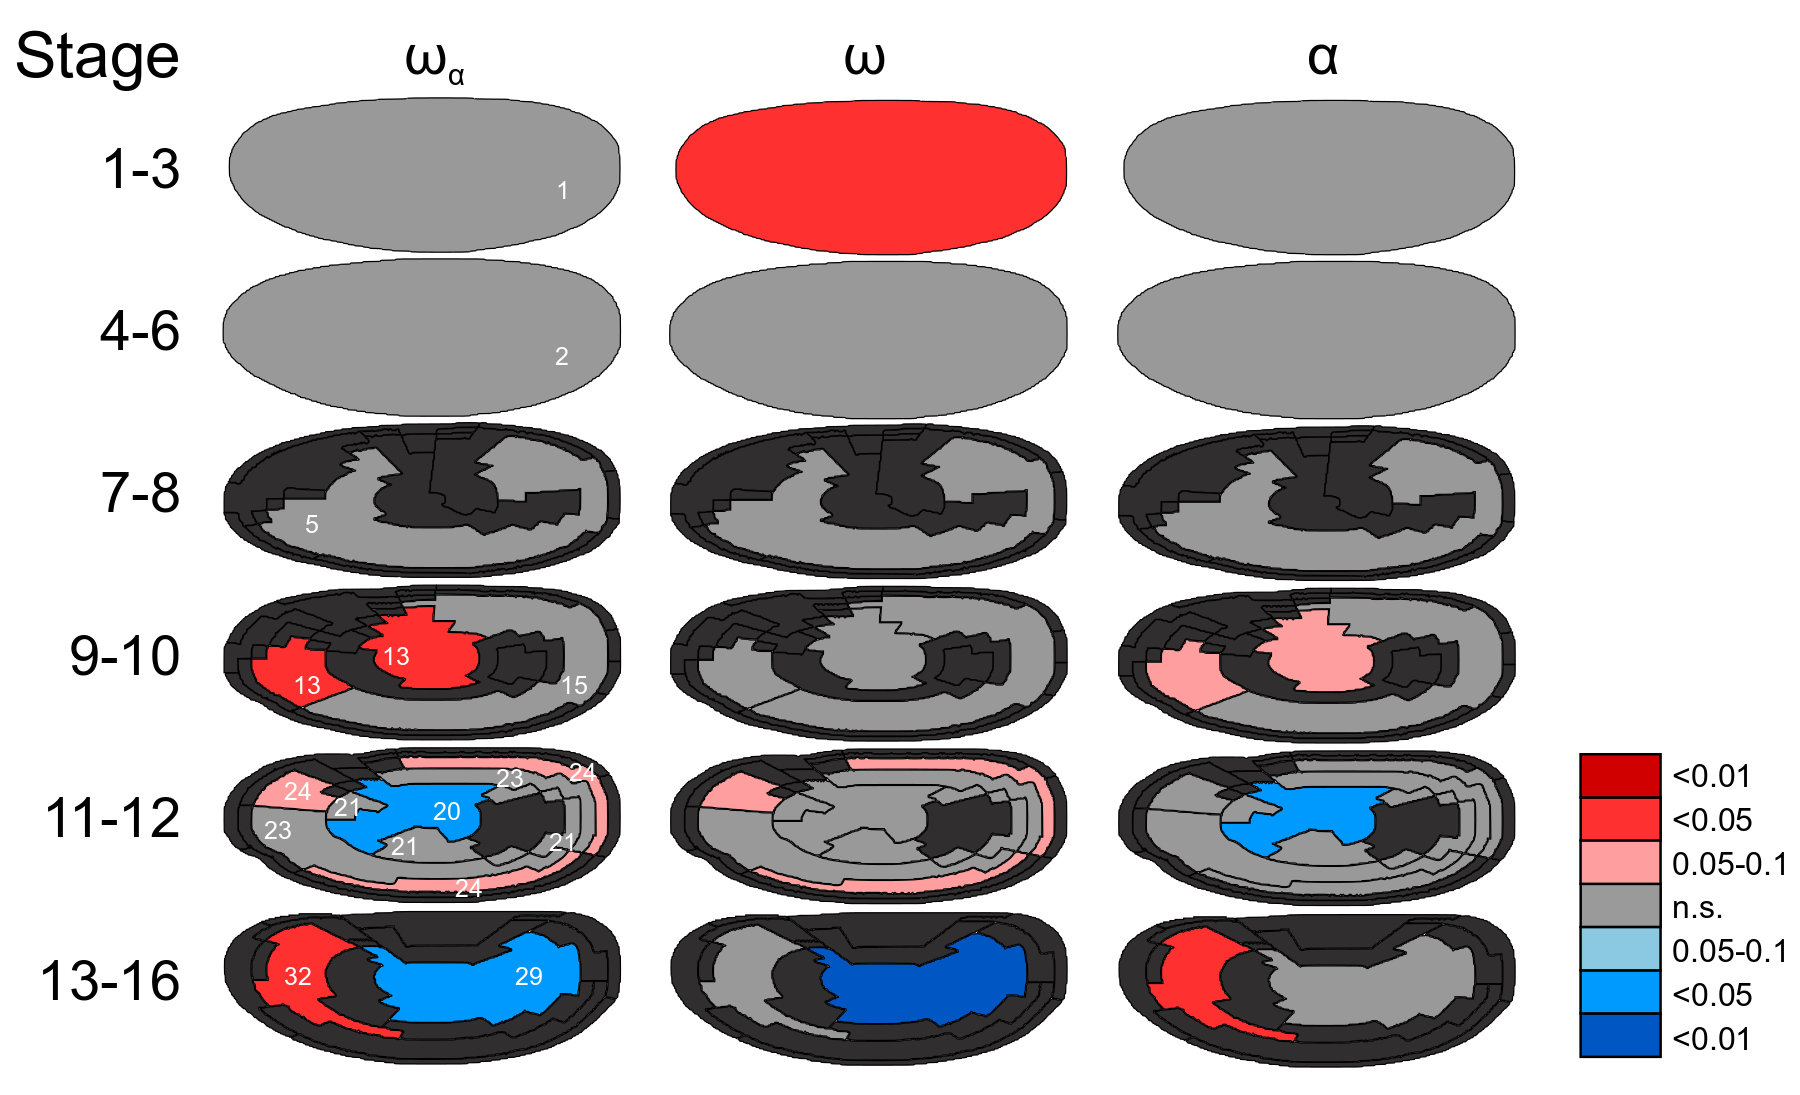
\includegraphics[width=0.7\textwidth]{./Images/Art-III/OmegaA_territories.png}
  \centering
  \caption{\textbf{$\omega_{\alpha}$ on embryonic territories over space and time.}
   Territories drawn in red in the central column mark significantly high $\omega_{\alpha}$ while those in blue mark significantly low $\omega_{\alpha}$ in space in each of the 6 developmental stages (rows). Other columns depict $\alpha$, the proportion of base substitutions fixed by natural selection, and $\omega$, the rate non-synonymous substitutions relative to the mutation rate. 
  Territories in dark gray are territories without enough specific genes to be analyzed. The statistical was calculated by a permutation test using all the genes analyzed (see Material and methods). Territory 13 in stage 9-10 ($\omega_{\alpha}$: 0.059, p = 0.045). Territory 20 from stage 11-12 ($\omega_{\alpha}$: 0.022, p = 0.048; $\alpha$: 0.259, p = 0.028). Territory 24 from stage 11-10 ($\omega_{\alpha}$: 0.070, p = 0.061). Territory 29 from stage 13-16 ($\omega_{\alpha}$: 0.037, p = 0.047; $\omega$: 0.074, p < 0.001). Territory 32 from stage 13-16 ($\omega_{\alpha}$: 0.068, p = 0.044; $\alpha$: 0.71, p = 0.04).
  }
  \label{fig:Art-III-OmegaA_territories}
\end{figure}
%%%%%%%%%%%%%%%%%%%%%%%%%%%%%%%%%%%%%%%%%%%%%%%%%%%%%%%%


\subsection{Transcriptome age index and other genomic determinants}
%bjective
Then, I wanted to test if the `age' of the genes, also differed between different parts of the embryo and how this related to the adaptation results. For that, I used the phylostratigraphic maps of \textit{D. melanogaster} \citep{Drost2015}, that assign a phylogenetic age to each protein-coding gene based on the phylogenetic level at which orthologs for a gene are found (a young found only in Drosophilids would be very young, of age 1). Also, I used a modified version of the Transcriptome Age Index (TAI; \citealp{Domazet-Loso2010}) and applied it to the polar regions and STs (see III, methods). TAI is low for regions expressing old genes and large for regions expressing young genes.
%
%%%%%%%%%%%%%%%%%%%%%%%%%%%%%%%%%%%%%%%%%%%%%%%%%%%%%%%%
\begin{figure}[h]
  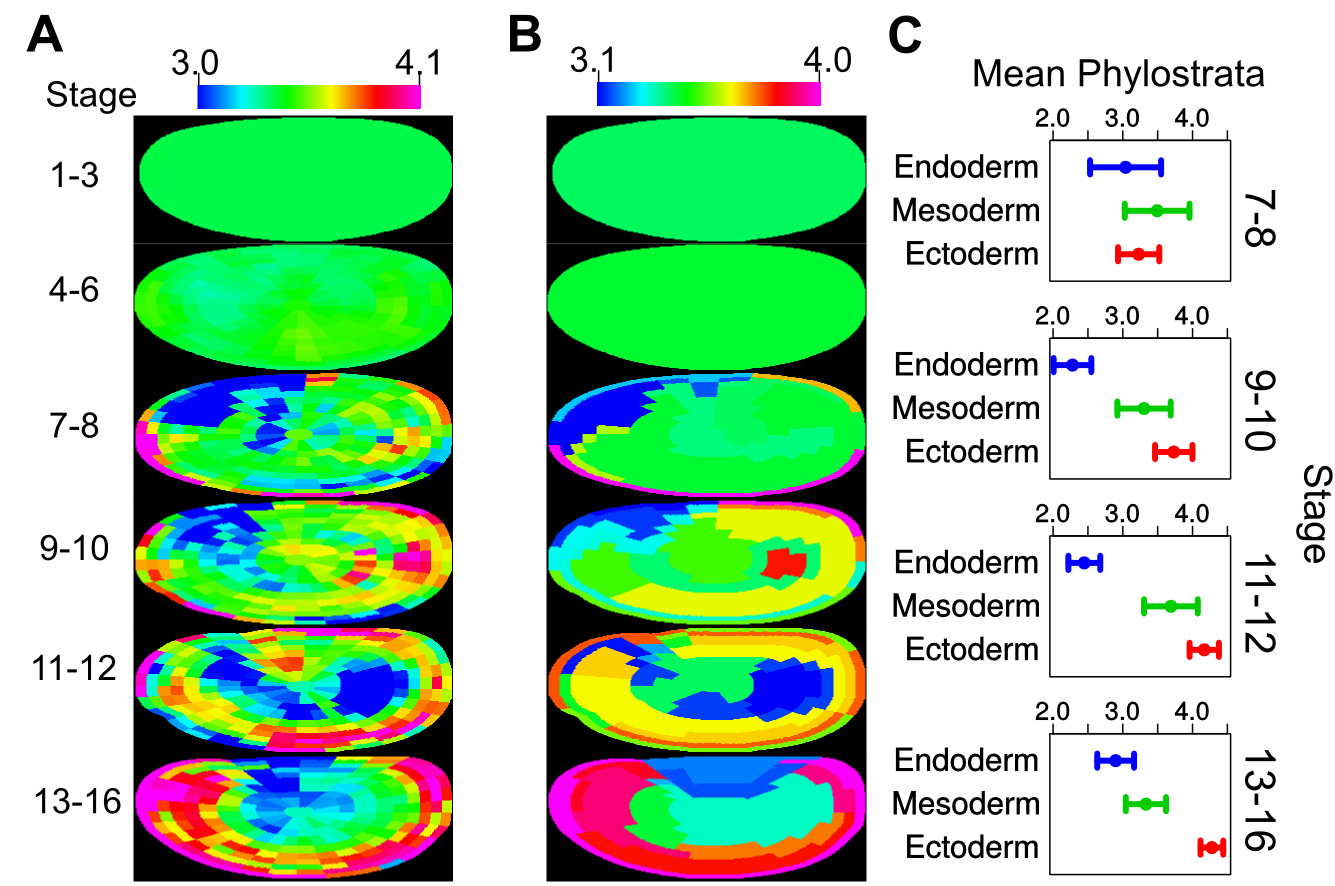
\includegraphics[width=0.7\textwidth]{./Images/Art-III/TAI.png}
  \centering
  \caption{\textbf{The center of the embryo expresses older genes.}
   (A) Heatmaps showing the transcriptome age index (TAI) im polar regions (B) Heatmaps showing the TAI for STs. (C) Mean phylostrata of genes assigned to each germ layer. Circles represent the mean and whiskers the SEM.
  }
  \label{fig:Art-III-TAI}
\end{figure}
	\nomenclature{SEM}{Standard error of the mean}
%%%%%%%%%%%%%%%%%%%%%%%%%%%%%%%%%%%%%%%%%%%%%%%%%%%%%%%%
%
%results TAI
I found that STs with low $\omega_{\alpha}$ express (on average) older genes (high TAI values). Similar results were found for anatomical structures (III, Fig. S2).
%
I also found that in stage 13-16 the mean phylogenetic age of the genes expressed in the endoderm is lower than in other germ-layers, specially compared to the ectoderm (Fig. \ref{fig:Art-III-TAI}).
Similar TAI results between germ-layers were found by \citet{Domazet-Loso2007} but without stages comparisons.
% discussion TAI
The correlation between adaptation and gene age fit the expectation that older genes would more likely perform essential functions than younger genes, and that, as older genes would have been moulded by natural selection for longer times would be therefore more close to optimality (assuming that this function is conserved). Therefore, more room for changes would be expectable in embryo regions with a larger proportion of younger genes. 

% results Codon Bias
I also found that embryo polar regions with high $\omega_{\alpha}$ have low codon bias (previously reported by  \citealp{Sharp1991,Betancourt2002,Haerty2007}) and that, as \citet{Plotkin2011} previously found, regions high codon bias show have high levels of gene expression (average RNAseq levels per region; III, methods).
To clarify the relation between these three variables, I fitted a multivariate linear regression and found that embryo regions with high $\omega_{\alpha}$ exhibit low codon bias relative to what would be expected from their gene expression levels (III, Fig 5).
%discussion codon bias
The negative correlation between codon bias and protein adaptation that I found would be expected given that, an adaptive  aminoacid change in a protein would be probably different from a change that would increase codon usage efficiency \citep{Hershberg2008,Presnyak2015}.
%Since codon bias also correlates with gene expression levels per region, high $\omega_{\alpha}$ should be found where codon usage is low relative to gene expression levels, as we observe

\subsection{Selective constraint in late embryogenesis}

Analysing the RNAseq developmental data from the modENCODE project \citep{Graveley2011} with the DFE-alpha method (IV, methods), I found that from hour 10 until 24 of embryogenesis show significant low $\omega_{\alpha}$ and $\omega$ (see Fig X in section X), which would be consistent with the low rate of adaptive change seen in many anatomical structures in stage 13-16 (as stage 13-16 of BDGP roughly maps to RNA-seq samples em10-12 hr, em12-14 hr, em14-16 hr, and em16-18 hr of modENCODE; \citealp{Hammonds2013}).
Therefore, by combining different approaches, I could identify that the proteins produced in late embryogenesis change less their aminoacid sequence (i.e., are more conserved). This phenomenon, of some proteins evolving slower, has been called `selective constraint' and has been linked to the higher degree of functionality of such proteins \citep{kimura1983neutral}.
Most importantly, I could identify which specific anatomical structures expressed genes with a higher degree of conservation.
%	\clearpage
\section{Adaptation trough \textit{Drosophila} life cycle (IV)}
	
\subsection{Temporal adaptation profile}

The results showed adaptation in two different periods in the life cycle of \textit{Drosophila}: 
1) in the earliest 2 hours of the embryo development ($\omega_{\alpha}$, $\omega_{d}$ and $\omega$ show their highest value at this stage) and 
2) from the L3 larval stage onwards, specially in the pupal and adult male stages which exhibit the highest levels of adaptive.

In between these stages of high adaptation, mid and late embryonic stages show high conservation. 
Similar results were found when considering after excluding immune system and testes genes (IV, Fig. S2) or when the mutation rate is estimated using the 4-fold degenerate sites (IV, Fig. S3).

The high adaptation rate in males is consistent with previous reports of higher adaptive substitutions in the genes expressed in males \citealp{Proschel2006,Haerty2007}). 
In contrast, based in a hybrid mis-expression assay with \textit{D. melanogaster} and \textit{D. sechellia}, \citet{Artieri2010} suggested a highly conserved pupal stage under strong stabilizing selection, which is contrary to the results shown in here, which indicate that, at least at the level of DNA coding sequence variation, pupal stages are among the least conserved.

As the morphology and other aspects of the phenotype of the larva and the adult arise primarily through the genetic, cellular and tissue interactions of embryonic and pupal development respectively, the adaptation in the larva or the adult morphology should be reflected in the genes expressed in embryonic development and pupal development, respectively.
Therefore, the evidence that most embryonic development shows low rates of adaptive change while the larva and pupa stages show higher rates of adaptative change suggests that there has been more adaptive changes in the adult morphology than in the larva morphology (between \textit{D. melanogaster} and \textit{D. yakuba}).

\subsection{Selective constraint in late embryogenesis} \label{OmegaA_late_embryo}

From hour 10 until 24 of embryogenesis show significant low $\omega_{\alpha}$ and $\omega$ (see Fig \ref{fig:Art-IV-OmegaA_lifecycle}), which would be consistent with the low rate of adaptive change seen in many anatomical structures in stage 13-16 seen in section \ref{embryo_low_Omega} (as stage 13-16 of BDGP roughly maps to RNA-seq samples em10-12 hr, em12-14 hr, em14-16 hr, and em16-18 hr of modENCODE; \citealp{Hammonds2013}).
Therefore, the two different approaches used in here (adaptation map in the embryo and adaptation through the life cycle) show that the proteins produced in late embryogenesis change less their aminoacid sequence (i.e., are more conserved). 
This phenomenon, of some proteins evolving slower, has been called "selective constraint" and has been linked to the higher degree of functionality of such proteins \citep{kimura1983neutral}.
Most importantly, I could identify which specific anatomical structures expressed genes with a higher degree of conservation.

%%%%%%%%%%%%%%%%%%%%%%%%%%%%%%%%%%%%%%%%%%%%%%%%%%%%%%%
\begin{figure}[t]
  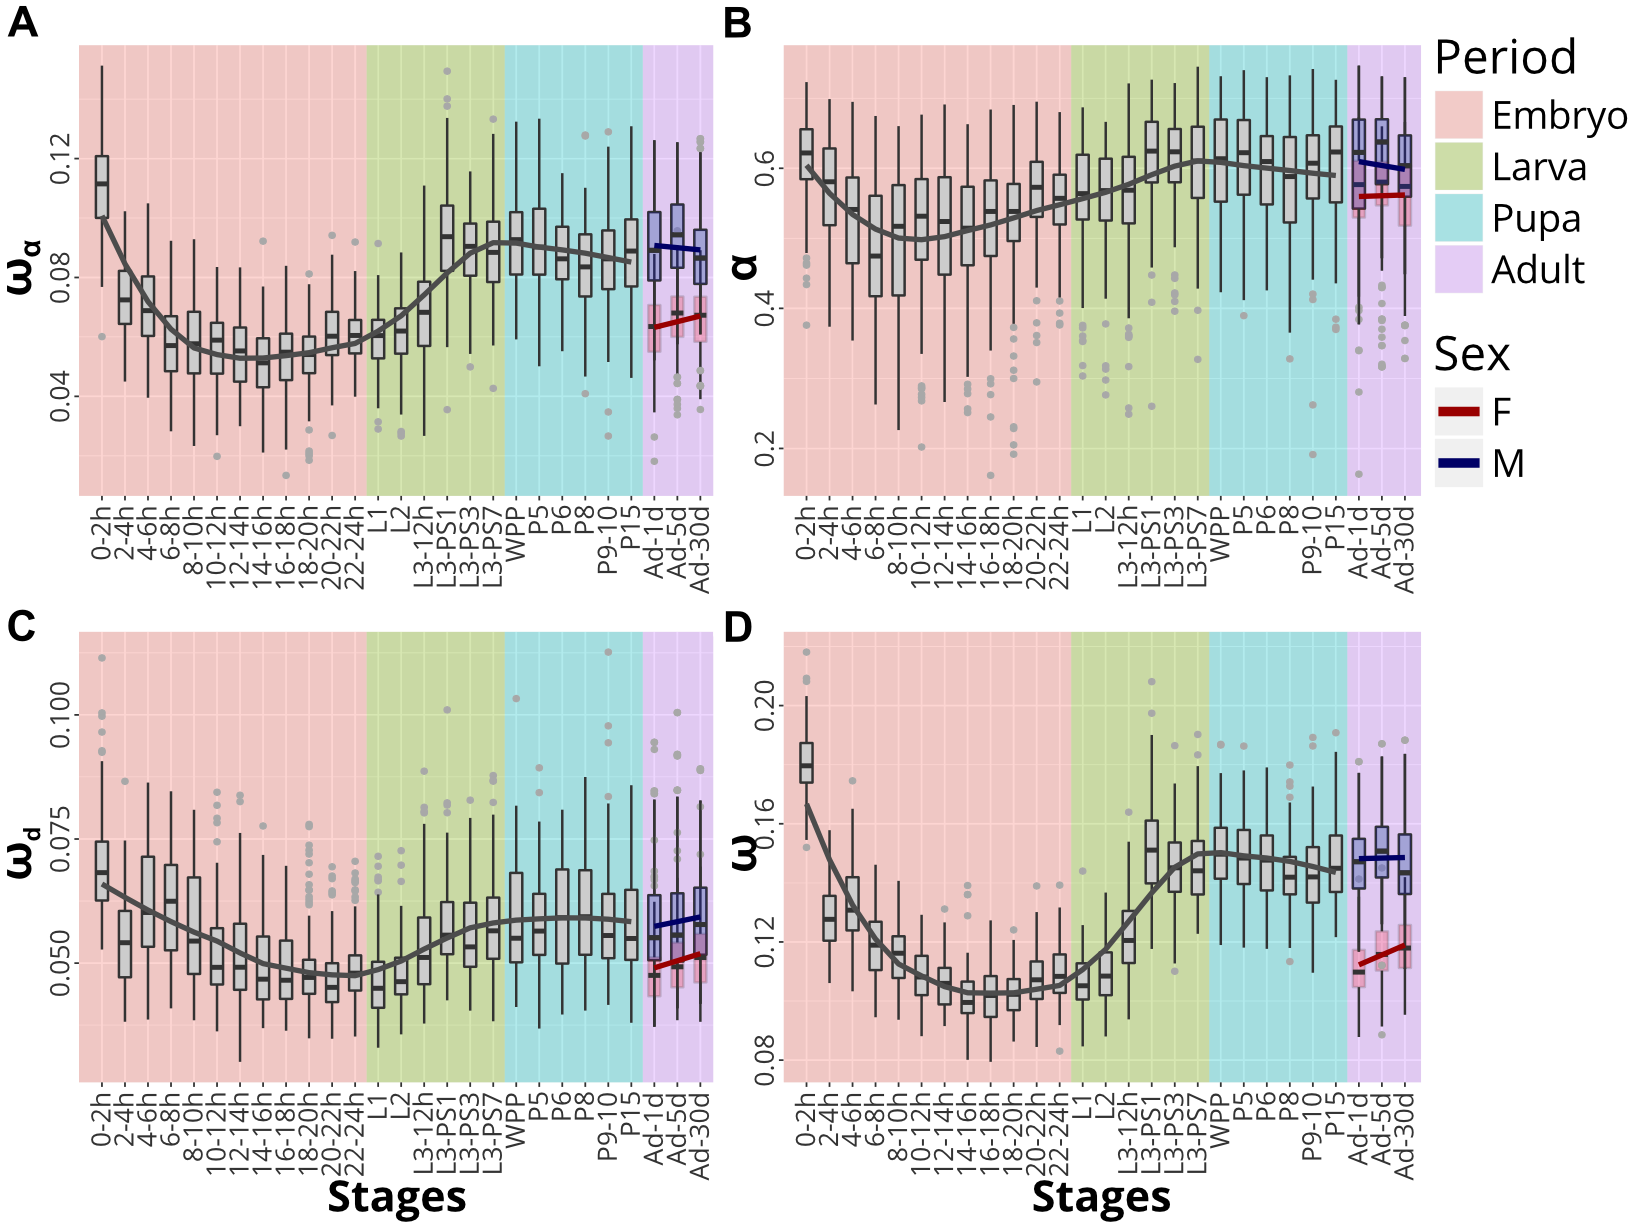
\includegraphics[width=\textwidth]{./Images/Art-IV/OmegaA_lifecycle.png}
  \centering
  \caption{\textbf{ {\large$\omega_{\alpha}$} (A),  {\large$\alpha$} (B), {\large$\omega_{d}$} (C), {\large$\omega$} (D) through the life cycle of \textit{D. melanogaster}} Each time point represents 1,000 random samples of 350 genes (with replacement) expressed in a stage. Red line represents a LOESS regression. Female and male stages are fitted to a linear regression. There are 12 embryonic stages at 2hr intervals (from 0h to 24h). Larval stages at first instar (L1), second instar (L2) and third instar (L3). L3 stages are subdivided into the first 12 hours (L3-12h) and several puff stage (L3-PS1 to L3-PS7). WPP is the white pre-pupae stage. Pupal stages are phanerocephalic pupa, 15h (P5), 25.6 hours pupa (P6), yellow pharate, 50.4 hours (P8), amber eye-pharate, 74.6 hours (P9-10), green meconium pharate, 96 hours (P15). Adult stages are 1, 5 and 30 days after eclosion (Ad-1d, Ad-5d, Ad-30d).
  }
  \label{fig:Art-IV-OmegaA_lifecycle}
\end{figure}
%%%%%%%%%%%%%%%%%%%%%%%%%%%%%%%%%%%%%%%%%%%%%%%%%%%%%%%%

\subsection{Results support the Hourglass model}

The temporal pattern of adaptation (and conservation) are roughly consistent with the Hourglass model (HG), specially for the early and mid embryonic development.
%This consistency is, however, rather weak since there are no major differences in ω between embryonic stages after the eight hour. 
During the first 6 hours $\omega$ and $\omega_{\alpha}$ are significantly high (permutation test), which is consistent with the expectations of the HG.
The same parameters are significantly lower during mid-embryogenesis, which is also consistent with the higher conservation expected from the HG, as the phylotypic stage (the most conserved stage) in \textit{Drosophila} has been suggested to be between the 6th and 10th hour \citep{Drost2015}.
However, during late embryonic stages (from 10-12h to 22-24h) $\omega$ and $\omega_{\alpha}$ are significantly lower (permutation test), which is not what is expected from the HG.

In contrast with some previous studies \citep{Davis2005,Kalinka2010} we do not find that the later stages of embryonic development are less conserved. 
It was found however, that a cluster composed of genes whose expression is high only in late development (done with a fuzzy clustering algorithm, cluster 8; see study IV), shows a significant $\omega$ and $\omega_{\alpha}$. In here, this group of genes have only a minor effect on the global pattern.
It could be that, due to the different methodology used by these other studies, these genes would have a relatively higher effect on the pattern observed. It could also be that the differences are partly due to the different species used in the analyses.\citet{Davis2005} use D. pseudoobscura as outgroup species while \citet{Kalinka2010} use six different \textit{Drosophila} species including \textit{D. melanogaster} but not \textit{D. yakuba}, the species used as outgroup in this work.

Despite these differences, the overall $\omega$ and $\omega_{\alpha}$ pattern (Fig \ref{fig:Art-IV-OmegaA_lifecycle}) is consistent with the HG model of embryonic development in \textit{Drosophila} \citep{Kalinka2010}.


%% result genomic determinants
\subsection{Correlation of adaptation with some genomic determinants}
Many "genomic determinants" temporal profiles correlate either positively other negatively with $\omega_{\alpha}$ (IV, Figs 2 and 3). 
%
Thus, messenger complexity (number of transcripts divided by the number of exons) correlates with $\omega_{\alpha}$ (rank correlation; see study IV). On the contrary, gene size, number of exons, codon usage bias and number of transcripts per gene negatively correlate with $\omega_{\alpha}$ (all with significant rank correlations; see study IV). 

This is consistent with previous studies that have shown that small gene size has been correlates with $\omega$ \citep{Duret1999,Comeron2012}.
%To our knowledge, the number of exons and transcripts themselves have never been directly associated with neither $\omega$ nor $\omega_{\alpha}$, as we found in our study.
It has also been suggested \citep{Gellon1998}, that developmental genes tend to have a complex gene structure with many exons and cis-regulatory elements and a complex regulation in space and time. Therefore, the correlations we observe between $\omega_{\alpha}$ and some genomic determinants is likely to simply reflect the fact that during mid-embryonic development, genes have a more complex spatio-temporal regulation and a more complex regulatory structure (as measure by the messenger complexity measure).

Based on the results shown in here, it is suggested that these genomic determinants can serve as predictors of adaptive change during development and that the temporal pattern of the genomic determinants are simply a consequence of the complex spatio-temporal regulation of gene expression occurring in embryonic 
development (as suggested on more qualitative grounds \citealp{Duboule1998}).

An important difference between this analysis and previous ones is that the DFE-alpha method allows to differentiate finely between conservation (indicated by low $\omega$), adaptive evolutionary substitution (high $\omega_{\alpha}$), non-adaptive substitution (high $\omega_{D}$) and the proportion of adaptive versus non-adaptive substitution (high $\alpha$). 
In a previous study, it was found that the 150 genes with the highest number of non-synonymous substitutions are expressed more strongly in larva and pupa than in embryo and that their highest level of expression is in male adults \citep{Davis2005}.
The work presented here would also be consistent with Davis et al., although in the latter case conservation and positive selection cannot be distinguished.



	\clearpage



%%%% -----------------------------------------------------------------
%%%% -----------------------------------------------------------------

\chapter{Concluding Remarks}

The study of organismal complexity during embryonic development presented here shows that there are commonalities and differences between \textit{D. melanogaster} and \textit{C. intestinalis}. Both species showed a non-linear increase in all complexity measures, while the most remarkable difference is the timing of the major change in complexity, which is earlier in \textit{D. melanogaster} (around gastrulation).
Another common pattern is the early increase in complexity when considering only transcription factors or growth factors (or other signalling molecules). This confirms the special role these genes have in early metazoan development. It could be therefore expected that the evidence presented here, regarding these type of genes, should be observed also in other species. 

One important result of this work is that within each species, the three complexity measures showed a similar pattern (even when it would not be necessarily the case; see section \ref{measures_relations}). This means that altogether, these measures (compartmentalization, disparity and roughness) are reflecting a global pattern of increase in complexity in each species. Therefore, it could be hypothesized that a similar increase in complexity would be found using alternative measures of complexity (e.g., spatial entropy). Further analysis would be required to test this hypothesis.
Also, the Synexpression Territories analysis allowed to "reconstruct" the main embryonic differentiation events in both species in a consistent manner with the current knowledge of the development of these model organisms and without focusing in specific genes.

The elaboration of an adaptation map on the fruit fly embryo can be considered a proof of concept of how the combination of diverse fields like evolutionary developmental biology and population genomics, and new techniques such as the phylostratigraphy, can be useful to give a fresh view on an old problem.
Using these maps, it was possible to visually identify that the center (internal part) of the embryo expresses a more conserved and older transcriptome, while the outside (external part) expresses phylogeneticaly younger and less conserved genes. This evidence seems to support the hypothesis of the antecedence of the endoderm with respect to the ectoderm \citep{Hashimshony2014}. It would be interesting to extend this adaptation mapping analysis for the entire development (until the adult stage) as it could be that in later stages, different structures or organs have been under positive or negative selection.

The estimation of adaptation over the entire life cycle of \textit{D. melanogaster}, as presented here, supports the HG model of development. We find, as other analyses previously have, that the mid-embryogenesis is highly conserved. The work presented here is different from previous ones in that it uses a more complete spatio-temporal dataset and a method that uses inter and intra-specific DNA coding variation to estimate, with an unprecedented precision, the proportion of adaptive changes.
Furthermore, as a result of this work is hypothesized that the hourglass model can be best predicted by various genomic features. However, further work is necessary to test this hypothesis.

The observed patterns of complexity and adaptation/conservation throughout the embryonic development of \textit{D. melanogaster} might be intricately connected.
%
The increase in spatial disparity of gene expression in late embryogenesis (Fig. \ref{fig:Art-I-3measures}),
which reflects that the different parts of the embryo express progressively more different combinations of genes, 
is likely related with the expression, at this specific developmental period, of genes with multiple expression domains.

At the same time, genes expressed in many different places and times during development would likely require an elaborate genetic structure (reflected in their exons number, intron length, transcripts number) which would permit such complex spatio-temporal regulation of their gene expression.
%
%
It could be then hypothesized that a mutation in such genes would have high pleiotropic effects (as they would affect many different parts of the embryo) which could result in stabilizing selection against mutational variation \citep{Galis2002}.
The correlation between specific genetic features intuitively related to spatio-temporal regulation of gene expression and the high level of conservation at late embryogenesis seems to support this hypothesis. A more precise analysis, which could disentangle all these variables is however required.

%
%SERIA BUENO TAMBIEN HACER ALGUN TIPO DE CONEXION ENTRE LO DE LA COMPLEJIDAD Y LO DE LA ADAPTACION EN EL ESPACIO O EN EL TIEMPO (EN EL TIEMPO SERIA MAS FACIL Y RELACIONARLO CON LO QUE DECIMOS DE LA CONSTRICCION EN LOS GENES DEL DESARROLLO DADO LA COMPLEJIDAD DE SU REGULACION.

%This thesis confirms that a statistical approach in developmental biology can provide valuable information on fundamental processes by describing their properties at a statistical level, beyond the role of individual genes.
This thesis confirms that a statistical approach in developmental biology can provide valuable information on fundamental processes by describing their properties at a statistical level, and therefore allows to attain a global view that transcends the role of individual genes.

%AQUI TAMBIEN PODRIAS DECIR QUE TU TESIS CONFIRMA QUE LA STATISTICAL DEVELOPMENTAL BIOLOGY PUEDE DECIR COSAS INTERESSANTES MAS ALLA DEL PAPEL DE CADA GEN (RELACIONADO CON LO QUE DICES AL PRINCIPIO DE LA INTRO SOBRE ESTO.
%In here, I have taken advantage of the great amount of information about developmental gene expression that has accumulated in many years from collective efforts of the developmental biology community. This great amount of accumulated data allows to shift the focus from single genes to a systemic approach in which the global statistical properties of development can be investigated.


\textbf{Future directions}

The emergence of new techniques, like "spatial transcriptomics" of tissue sections at single-cell resolution \citep{Stahl2016} could make possible to have information, derived from a single experiment, of all the genes expressed in a 2D section of an embryo. The application of the measures presented here could be apply to this kind of data in a straightforward manner, solving the limitation in resolution of the work presented here.

It is important to mention that this work has used differential gene expression in the embryo and its spatial distribution as a tool to investigate complexity. However, embryonic development can not be reduced to differential gene expression. Cellular behaviours and the physical properties of the cells and tissues have also a causal role in the developmental process. It would be interesting to be able to measure the differential apportionment to complexity increase of the different developmental mechanisms.


The increase of organismal complexity and the study of adaptation during development remain fascinating topics after many centuries, and still offer many open questions to be solved. The incredibly fast pace of data generation, the development of new techniques and sophisticated methods give hope to finally open the black box of development.

QUIZAS PODRIAS DECIR QUE ESTA MISMA APROXIMACION SERA POSSIBLE PROXIMAMENTE EN OTROS TIPOS DE DATOS COMO EN IMAGINAL DISC (DONDE IGUAL SALE UNA BASE DE DATOS DE EXPRESSION), Y PARA RATON Y HUMANOS Y QUIZAS C.ELEGANS.

%%%%%% for results of compartmentalization
%
%It could be expected that these early increase in complexity in drosophila is shared by all insects with a syncitial blastoderm stage. It could be that there are differences between these based on the number of cell divisions until the blastoderm is cellularized. It is known that Drosophila cellularizes relatively late (so there is more time for patterning within the syncitial bastoderm). In contrast, the desert locust (Schistocerca gregaria) cellularization occurs very early, before the formation of the blastoderm (REF Ho).
%
%The rapid development in drosophila could be due to selective pressures on the time of development, caused by the the eggs being layed ephemeral resources such as decaying fruits (this classical view has been chalenged recently; reviewed in REF Prasad). 
%The embryonic development of D. melanogaster takes around 1 day at 22 degrees. Even when developmental time can vary in a three fold manner depending on the Drosophila species and temperature (D. virilis embryonic development at 18 C takes more than 45 hours, compared to less tha 15 hours at 30 C in D. ananassae: REF Kuntz), it can be considered fast compared the dessert locust. In the locust, embryonic development takes around two weeks in calid environments in West Africa but it can take up to 70 days in the cooler temperatures of North Africa (REF locushanbbook).
%
%Also, it would be interesting to know if there are some differences between the two main modes of segmentation in insects, i.e., short germband and long germband. The red bettle (Tribolium castaneum) is most popular short germband inset that serves as a developmental biology model organism. Many valuable resources have become available in the last decades/years (REF Bucher). 
%
%
%The period of egg development, between laying and hatching, is called the incubation period. The rate at which eggs develop varies according to the soil temperature. For example, in the summer breeding areas of West Africa, the Red Sea coast and lowland India the incubation period takes 10-14 days but this is extended to 25-30 days in the cooler spring breeding areas of central Arabia, southern Iran and Pakistan while in North Africa it can take as long as 70 days in exceptionally cold weather

\clearpage
%%%% -----------------------------------------------------------------
%%%% -----------------------------------------------------------------

%\listoffigures
%\printnomenclature
%%%% -----------------------------------------------------------------
%%%% -----------------------------------------------------------------
%\bibliographystyle{plain}

%%%%% The bibliography is written in a small fontsize and in 2 columns
\begin{multicols}{2}
{\footnotesize
\bibliography{Bibliography}
}
\end{multicols}

%%%% -----------------------------------------------------------------
%%%% -----------------------------------------------------------------
\end{document}